\documentclass{ConfigurationFiles/PoliMi3i_thesis}


% CONFIGURATIONS
\usepackage{parskip} % For paragraph layout
\usepackage{setspace} % For using single or double spacing
\usepackage{emptypage} % To insert empty pages
\usepackage{multicol} % To write in multiple columns (executive summary)
\setlength\columnsep{15pt} % Column separation in executive summary
\setlength\parindent{0pt} % Indentation
\raggedbottom
\usepackage{multirow}

% PACKAGES FOR TITLES
\usepackage{titlesec}
% \titlespacing{\section}{left spacing}{before spacing}{after spacing}
\titlespacing{\section}{0pt}{3.3ex}{2ex}
\titlespacing{\subsection}{0pt}{3.3ex}{1.65ex}
\titlespacing{\subsubsection}{0pt}{3.3ex}{1ex}
\usepackage{color}

% PACKAGES FOR LANGUAGE AND FONT
\usepackage[english]{babel} % The document is in English  
\usepackage[utf8]{inputenc} % UTF8 encoding
\usepackage[T1]{fontenc} % Font encoding
\usepackage[11pt]{moresize} % Big fonts

% PACKAGES FOR IMAGES
\usepackage{graphicx}
\usepackage{transparent} % Enables transparent images
\usepackage{eso-pic} % For the background picture on the title page
\usepackage{subfig} % Numbered and caption subfigures using \subfloat.
\usepackage{tikz} % A package for high-quality hand-made figures.
\usetikzlibrary{}
\graphicspath{{./images/}} % Directory of the images
\usepackage{amsthm} % Coloured "Theorem"
\usepackage{thmtools}
\usepackage{xcolor}
\usepackage{float}

% STANDARD MATH PACKAGES
\usepackage{amsmath}
\usepackage{amssymb}
\usepackage{amsfonts}
\usepackage{bm}
\usepackage[overload]{empheq} % For braced-style systems of equations.
\usepackage{fix-cm} % To override original LaTeX restrictions on sizes

% PACKAGES FOR TABLES
\usepackage{tabularx}
\usepackage{longtable} % Tables that can span several pages
\usepackage{colortbl}

% PACKAGES FOR ALGORITHMS (PSEUDO-CODE)
\usepackage{algorithm}
\usepackage{algorithmic}


% PACKAGES FOR REFERENCES & BIBLIOGRAPHY
\usepackage[
    colorlinks=true,
    linkcolor=black,
    anchorcolor=black,
    citecolor=black,
    filecolor=black,
    menucolor=black,
    runcolor=black,
    urlcolor=black
]{hyperref} % Adds clickable links at references
\usepackage{cleveref}
\usepackage[square, numbers, sort&compress]{natbib} % Square brackets, citing references with numbers, citations sorted by appearance in the text and compressed
\bibliographystyle{abbrvnat} % You may use a different style adapted to your field

% OTHER PACKAGES
\usepackage[normalem]{ulem}
\usepackage{verbatim}
\usepackage[super]{nth}
\usepackage{pdfpages} % To include a pdf file
\usepackage{afterpage}
\usepackage{lipsum} % DUMMY PACKAGE
\usepackage{fancyhdr}
\usepackage{wasysym} % For the headers
\usepackage{rotating}
\usepackage{listings}
\usepackage{hyperref}
\usepackage{enumitem}
\input{ConfigurationFiles/alloy.sty}
\fancyhf{}

% Input of configuration file. Do not change config.tex file unless you really know what you are doing. 
% Define blue color typical of polimi
% Define blue color typical of polimi
% Define blue color typical of polimi
\definecolor{bluepoli}{cmyk}{0.4,0.1,0,0.4}

% Custom theorem environments
\declaretheoremstyle[
    headfont=\color{bluepoli}\normalfont\bfseries,
    bodyfont=\color{black}\normalfont\itshape,
]{colored}

% Set-up caption colors
\captionsetup[figure]{labelfont={color=bluepoli}} % Set colour of the captions
\captionsetup[table]{labelfont={color=bluepoli}} % Set colour of the captions
\captionsetup[algorithm]{labelfont={color=bluepoli}} % Set colour of the captions

\theoremstyle{colored}
\newtheorem{theorem}{Theorem}[chapter]
\newtheorem{proposition}{Proposition}[chapter]

% Enhances the features of the standard "table" and "tabular" environments.
\newcommand\T{\rule{0pt}{2.6ex}}
\newcommand\B{\rule[-1.2ex]{0pt}{0pt}}

% Pseudo-code algorithm descriptions.
\newcounter{algsubstate}
\renewcommand{\thealgsubstate}{\alph{algsubstate}}
\newenvironment{algsubstates}
{\setcounter{algsubstate}{0}%
\renewcommand{\STATE}{%
    \stepcounter{algsubstate}%
    \Statex {\small\thealgsubstate:}\space}}
{}

% New font size
\newcommand\numfontsize{\@setfontsize\Huge{200}{60}}

% Title format: chapter
\titleformat{\chapter}[hang]{
    \fontsize{50}{20}\selectfont\bfseries\filright}{\textcolor{bluepoli} \thechapter\hsp\hspace{2mm}\textcolor{bluepoli}{|   }\hsp}{0pt}{\huge\bfseries \textcolor{bluepoli}
}

% Title format: section
\titleformat{\section}
{\color{bluepoli}\normalfont\Large\bfseries}
{\color{bluepoli}\thesection.}{1em}{}

% Title format: subsection
\titleformat{\subsection}
{\color{bluepoli}\normalfont\large\bfseries}
{\color{bluepoli}\thesubsection.}{1em}{}

% Title format: subsubsection
\titleformat{\subsubsection}
{\color{bluepoli}\normalfont\large\bfseries}
{\color{bluepoli}\thesubsubsection.}{1em}{}

% Shortening for setting no horizontal-spacing
\newcommand{\hsp}{\hspace{0pt}}

\makeatletter
% Renewcommand: cleardoublepage including the background pic
\renewcommand*\cleardoublepage{%
    \clearpage\if@twoside\ifodd\c@page\else
    \null
    \AddToShipoutPicture*{\BackgroundPic}
    \thispagestyle{empty}%
    \newpage
    \if@twocolumn\hbox{}\newpage\fi\fi\fi}
\makeatother

%For correctly numbering algorithms
\numberwithin{algorithm}{chapter}




\definecolor{dkgreen}{rgb}{0,0.6,0}
\definecolor{gray}{rgb}{0.5,0.5,0.5}
\definecolor{mauve}{rgb}{0.58,0,0.82}

\lstset{frame=tb,
    language=alloy,
    aboveskip=3mm,
    belowskip=3mm,
    showstringspaces=false,
    columns=flexible,
    basicstyle={\small\ttfamily},
    numbers=none,
    numberstyle=\tiny\color{gray},
    keywordstyle=\bf\color{blue},
    commentstyle=\it\color{dkgreen},
    stringstyle=\color{mauve},
    breaklines=true,
    breakatwhitespace=true,
    tabsize=3
}

%----------------------------------------------------------------------------
%	BEGIN OF YOUR DOCUMENT
%----------------------------------------------------------------------------



\begin{document}
    \fancypagestyle{plain}{%
        \fancyhf{} % Clear all header and footer fields
        \fancyhead[RO,RE]{\thepage} %RO=right odd, RE=right even
        \renewcommand{\headrulewidth}{0pt}
        \renewcommand{\footrulewidth}{0pt}}

        
    \pagestyle{empty} % No page numbers
    \frontmatter % Use roman page numbering style (i, ii, iii, iv...) for the preamble pages

    \puttitle{
        title=Software Engineering 2\\Requirements Analysis and\\Specification Document,
        name1=Francesco Rausa - 10833982, % Author Name and Surname
        name2=David Ravelli - 10843295,
        name3=Pietro Poggi - 10891051,
        academicyear=2025-2026,
        version=1.0,
        releasedate=23/12/2025
          }
    
    
    \startpreamble
    \setcounter{page}{1} % Set page counter to 1


% TABLE OF CONTENTS
    \thispagestyle{empty}
    \tableofcontents % Table of contents
    \thispagestyle{empty}
    \cleardoublepage

    
    \addtocontents{toc}{\vspace{2em}} % Add a gap in the Contents, for aesthetics
    \mainmatter % Begin numeric (1,2,3...) page numbering


    \chapter{Introduction}
    \label{ch:introduction}%
    \section{Purpose}
In recent years, the use of bicycles has significantly increased, both as a means of daily transportation and as part of urban sustainability initiatives.
However, despite this growing interest, it remains difficult for cyclists to access reliable and up-to-date information about existing bike paths, their conditions, and potential obstacles along the way.
Such a lack of information often makes it challenging to plan safe, efficient, and enjoyable routes, discouraging many users from adopting cycling as a regular mode of transport.

\textbf{Best Bike Paths (BBP)} is designed to overcome these limitations by providing a collaborative and intelligent platform that collects, analyzes, and shares data about cycling routes.
Through the combination of user-generated content and automated data collection from mobile sensors, BBP enables users to record their trips, monitor their performance, and contribute to a shared, continuously updated map of bike paths.

The system also integrates external weather information to enhance the understanding of riding conditions, and it supports recommendation features to suggest the best paths between two points based on quality, safety, and user preferences. %non mi pare che ci siano preferenze espresse dai ciclisti

\label{sec:purpose}%

\subsection{Goals}
\label{subsec:goals}%
\newcounter{g}
\setcounter{g}{1}
\newcommand{\cg}{\theg\stepcounter{g}}

\newcounter{subg}
\setcounter{subg}{1}
\newcommand{\csubg}{\thesubg\stepcounter{subg}}
\newcommand{\resetsubg}{\setcounter{subg}{1}}
In this section, there are defined the goals that the system has to achieve:

    \uline{\textbf{Profile Management and Personal Tracking}}
    
        \textbf{[G\cg]} Registered users should be able to manage their profile on the platform.

        \textbf{[G\cg]} Registered users should be able to record and store their bike trips.

    \uline{\textbf{Bike Path Information Insertion and Management}}
    
        \textbf{[G\cg]} The system should provide detailed statistics about recorded trips (distance, average speed, performance metrics).

        \textbf{[G\cg]}  Registered users should be able to manually insert information about bike paths.

        \textbf{[G\cg]}  Registered users should be able to automatically insert information about bike paths through data acquisition from mobile devices.

        \textbf{[G\cg]}  Users should be able to confirm or correct automatically acquired information before publication.

        \textbf{[G\cg]}  Users should be able to make the inserted path information publishable.

    \uline{\textbf{Consultation and Visualization}}
    
        \textbf{[G\cg]} Users should be able to consult information about available bike paths. %ma anche quelli non registrati?

        \textbf{[G\cg]}  Users should be able to visualize on a map the bike paths between a specified origin and destination.

        \textbf{[G\cg]}  The system should calculate and display a score for each path based on its status and effectiveness.

    \uline{\textbf{Data Aggregation}}

        \textbf{[G\cg]}  The system should aggregate information coming from multiple users about the same paths, considering data freshness and number of confirmations.

    \uline{\textbf{Data Enrichment}}

        \textbf{[G\cg]}  The system should enrich trip data with meteorological information when available.

    


    
        


    \chapter{Overall Description}
    \label{ch:overall_description}%
    \section{Product Perspective}
\label{sec:product_Perspective}

\subsection{Scenarios}
\label{subsec:scenarios}

\item \textbf{1st Scenario: User Registration and Profile Management}\\
Elena Rossi, an avid cyclist and member of a local biking association, decides to join the BBP platform to keep track of her cycling activity and share information with other bikers. 
Upon opening the application, she selects the \textit{Sign Up} option. BBP prompts her to enter her personal details such as name, email, and password. Once the verification process is complete, Elena accesses her personal profile page. She updates her information, adds a short description of her cycling interests, and enables location permissions. From this moment, Elena becomes a registered user, able to record her trips and contribute data about bike paths.

\item \textbf{2nd Scenario: Recording and Viewing a Trip with Statistics}\\
Fausto Coppi is training for his next Tour. Fausto decides to record his rides using BBP. Before starting, he opens the app and presses \textit{Start Trip Recording}. 
During the ride, the app collects GPS data to track his route and speed. Once he arrives at his destination, he presses \textit{Stop}. The system automatically saves his trip and calculates key statistics: total distance, average speed, and travel time. Fausto later accesses his trip history, where he can review all his recorded rides, compare performances, and track his progress over time.

\item \textbf{3rd Scenario: Manual Insertion of Path Information}\\
During one of her rides, Federica Conti, an environmental engineering student and urban cyclist, discovers a newly built cycling lane that is not yet available on BBP’s map. 
After returning home, she opens the \textit{Add Path} section and manually inserts the details: the street names, total distance, surface quality, and current condition (e.g., \textit{Optimal}). She also reports a minor obstacle—a small pothole near a crossroad. After submitting, the system stores the path information, marking it as pending publication until Federica decides to make it public.

\item \textbf{4th Scenario: Automatic Path Detection and User Confirmation}\\
Marco Bianchi, a competitive cyclist who trains daily, prefers to let the system work automatically. 
Before starting his ride, he opens BBP and enables the \textit{Automatic Path Tracking} option, which allows the app to record his route and detect potential obstacles without manual intervention. 
When he starts cycling, BBP detects his movement and recognizes that he is riding. The system begins to collect GPS data and sensor readings from the accelerometer and gyroscope. 
After completing the trip, Marco receives an automatic summary of the detected path and potential obstacles identified by the sensors. He notices that BBP has mistakenly flagged a bump as a pothole, so he corrects the information before confirming the path. Once validated, the path is saved in his account..

\item \textbf{5th Scenario: Publishing a Recently Completed Path}\\
After reviewing and confirming the data from her latest ride, Sofia Moretti, an experienced city biker, decides to share it immediately with other cyclists. 
As soon as she finishes the trip and validates the automatically collected information, BBP prompts her with an option to \textit{Publish Path Information}. 
Sofia confirms the publication request, and the system instantly adds the path data to the public database, updating the collaborative map of available routes. 
Within moments, the new path becomes visible to all users of the platform.

\item \textbf{6th Scenario: Publishing a Previously Stored Path}\\
Two weeks later, Andrea Ricci, a cycling enthusiast who often explores rural routes, revisits one of his older recorded trips, which he never published. He reviews the path, adds updated comments about its current condition, and decides to share it with the community. 
He clicks \textit{Publish}, and BBP processes the data, making it available in the shared inventory. The system automatically merges his contribution with existing information about the same route, if available, ensuring that the most recent and confirmed data are displayed.

\item \textbf{7th Scenario: Consulting and Choosing a Path (Registered User)}\\
Francesco Leone, a registered cyclist who commutes daily by bike, plans a weekend trip across the city. He logs into BBP and specifies his origin and destination. 
The system searches the database for suitable routes and displays multiple options on the map, sorted by their score—considering factors such as safety, condition, and efficiency. 
Since Francesco’s profile indicates a preference for smoother surfaces and minimal traffic, BBP’s recommendation system automatically prioritizes such routes in the results. 
After reviewing the suggested paths, Francesco selects one and saves it as his chosen itinerary for the day.

\item \textbf{8th Scenario: Consulting and Choosing a Path (Unregistered User)}\\
Marta Villa, a casual cyclist who enjoys leisure rides on weekends, wants to discover new paths without creating an account. She opens the BBP app without logging in and accesses the public map. 
BBP displays all available paths but without personalized recommendations. Marta browses the map, filters by \textit{Optimal} status, and selects a route along the lakeside. Although she cannot record trips or add data, she can still view general information, such as total length, average condition, and user comments.

\item \textbf{9th Scenario: Updating Information on an Existing Path}\\
During a weekly commute, Tommaso Greco, a frequent user of BBP, rides along a route previously marked as \textit{Optimal}. He notices that a section of the track has recently deteriorated and requires maintenance. 
Once he finishes the ride, he opens BBP and selects \textit{Update Path Information}. He searches for the existing path and updates its condition from \textit{Optimal} to \textit{Requires Maintenance}. 
The system records his update and automatically aggregates it with reports from other users who have recently traveled the same route. 
By considering both the number of confirmations and the recency of the available data, BBP determines the most reliable current status of the path and updates its classification accordingly.

\end{itemize}

\subsection{Domain-level Class Diagram}
\label{subsec:domain_level_class_diagrams}

\begin{figure}[H]
    \begin{center}
        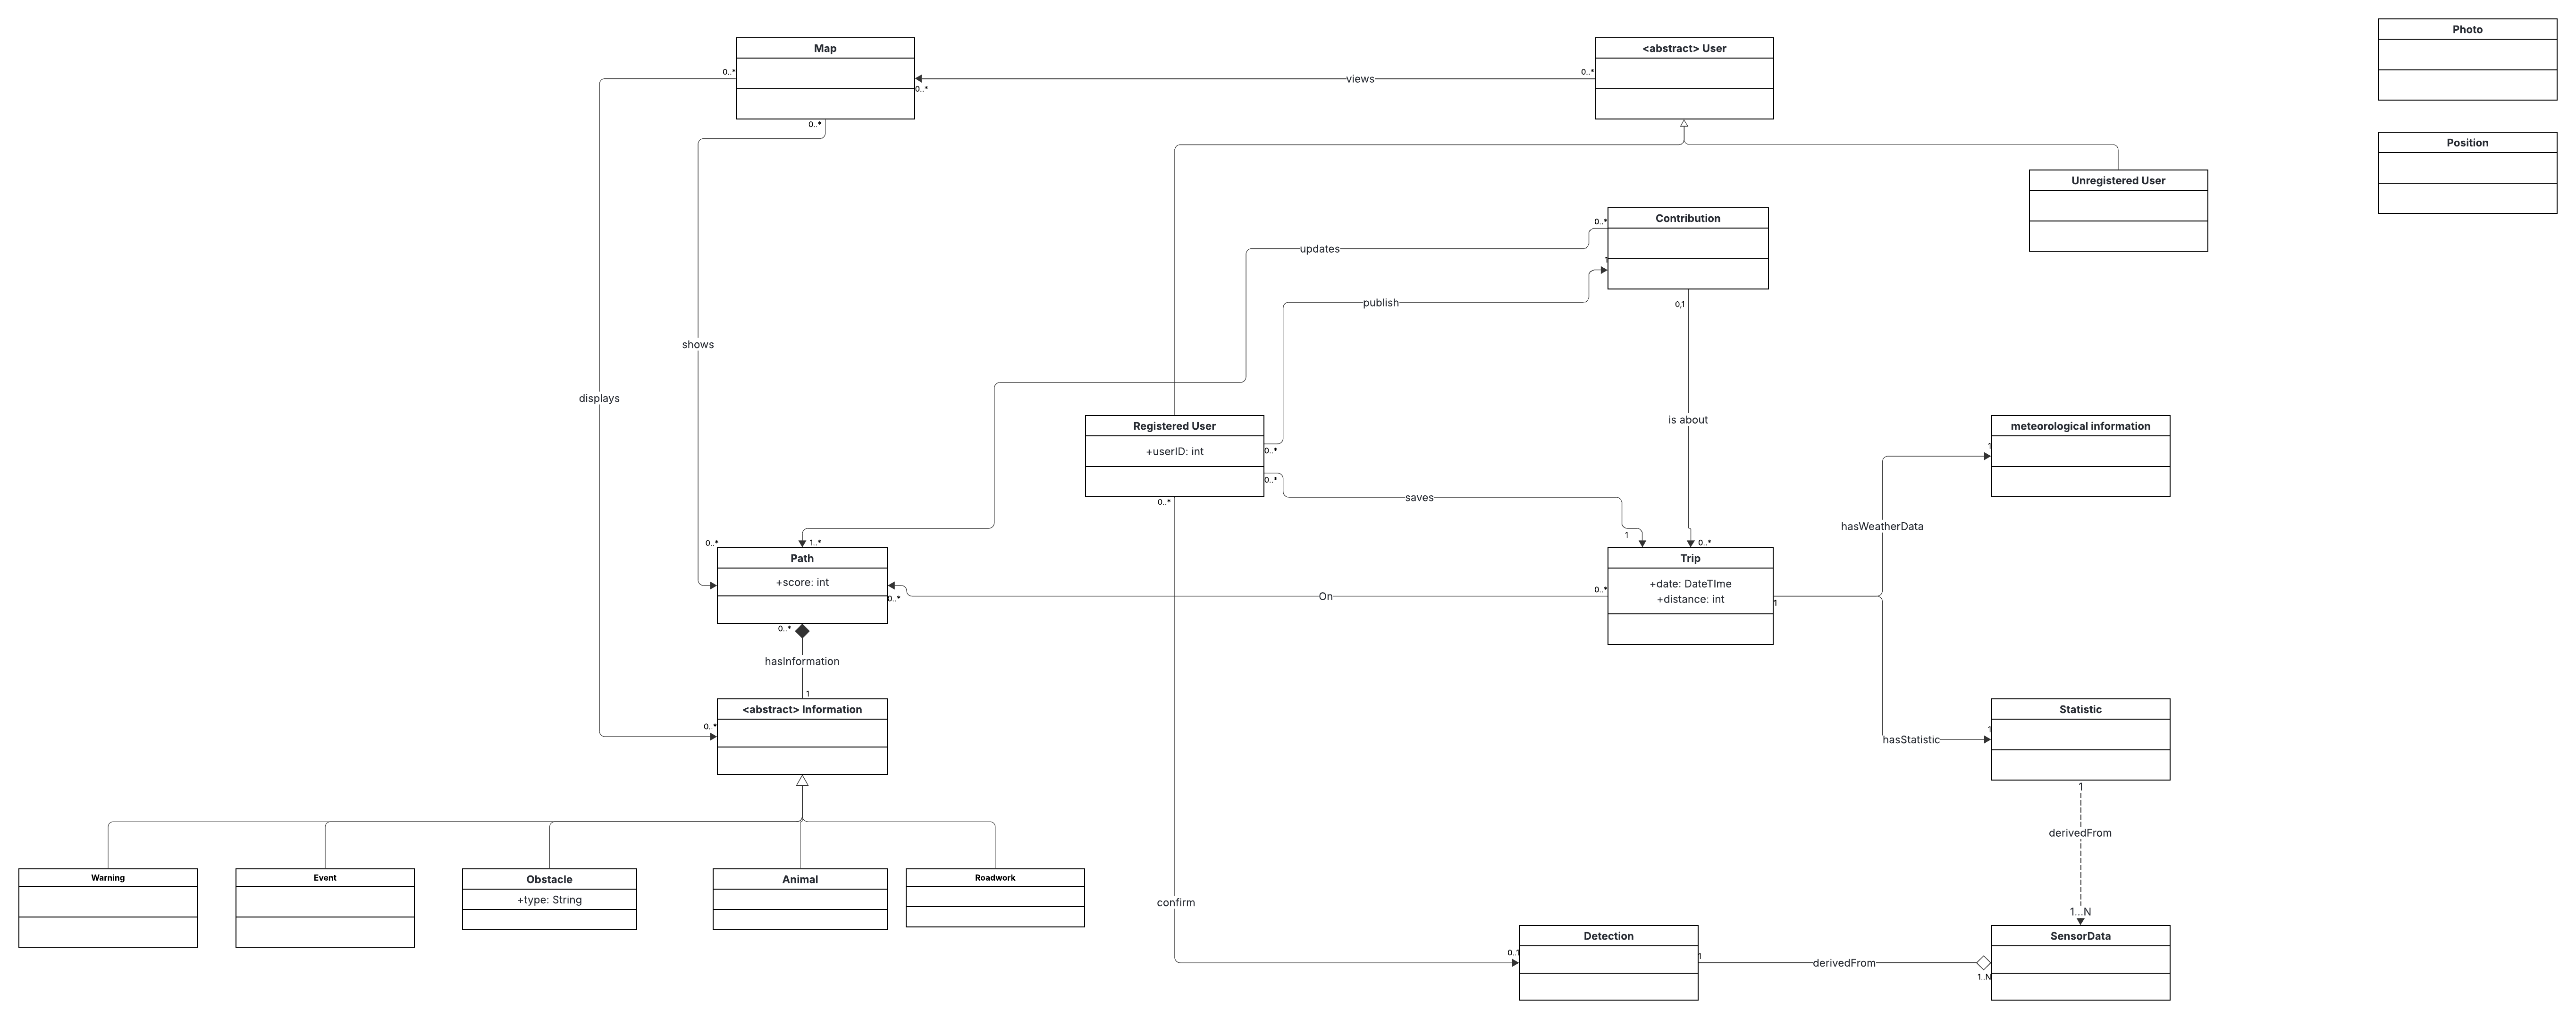
\includegraphics[width=0.9\linewidth]{RASD/Version1.0/images/UML class.png}
        \caption{Domain-Level Class Diagram.}
        \label{fig:domain_level_class_diagrams}
    \end{center}
\end{figure}

The entities interacting with the system are modeled through a hierarchical user structure in order to capture the capabilities and permissions required by the application. At the top level, the abstract User class generalizes any individual who accesses the application, whether simply browsing the map and available paths or actively contributing new information. In particular, the \textit{RegisteredUser} class extends User and enables all advanced features such as recording trips, confirming detections, and publishing contributions, while \textit{UnregisteredUser} supports basic navigation and map viewing functions.


The central concept of the application is the \textit{Contribution}, representing any information about the cycling network produced by a user or inferred automatically from sensor data. A contribution is always associated with a Path, and describes events or obstacles that affect that route. Contributions can be published directly by registered users (manual contributions), or generated via the confirmation of automatic detections performed during a trip. Each contribution updates the set of facts associated with a path and can include attachments such as photos or geographical positions for increased detail. The publication mechanism allows users to decide when their contributions become visible to all map viewers and impact the quality and usability scoring of each path segment.


The \textit{Path} entity models the infrastructure of the cycling network, comprising static segments that connect origins and destinations. Each path aggregates multiple pieces of Information—an abstract class that generalizes the different kinds of facts and events reported about the network. Its concrete subclasses include \textit{Warning, Event, Obstacle, Animal, and Roadwork}, each expressing specific types of phenomena detected or reported. The composition between path and information structures a dynamic collective history, while an explicit score attribute summarizes overall path safety or comfort, based on contributions and validations received.


The \textit{Trip} entity represents a specific cycling session recorded by a registered user. Each trip is associated with the user who performed it, stores basic data such as the date and distance, and can be complemented by additional statistical summaries (via the Statistic class) and meteorological data. Statistics are derived from raw \textit{SensorData} sampled during the ride, allowing the application to analyze detailed route conditions, travel patterns, and support more accurate detections of issues.


The detection process is modeled by the \textit{Detection} class, which represents the outcome of automatic analysis on a user's trip. When sensor data collected during a trip suggests the presence of a possible obstacle, the system generates a detection linked to that trip and to the affected path segment. Detections remain private and require explicit user confirmation: when a registered user reviews their trip, they confirm whether the suggested detection was a genuine obstacle encountered during the ride. Only upon confirmation does the system create or update a related Contribution, associating the appropriate \textit{Information} subtype (such as \textit{Obstacle} or \textit{Roadwork}) to the Path. Unconfirmed or rejected detections do not affect public contributions and path information. In this way, detections act as an intermediate, trip-specific representation that requires user validation, while contributions are the authoritative model for updating the infrastructure database.


The \textit{Map} entity models the application’s visualization layer. It displays all available paths, their associated contributions and information, and overlays real-time obstacles and statistics to let users plan their journeys. Any user can select a start and end point on the map; the system calculates the path, presents the obstacles detected, and helps choose the safest or most comfortable route.


Optional multimedia and localization enrichment is supported by the \textit{Photo} and \textit{Position} entities. Positions specify geographic coordinates for a point along a path, while photos can visually document the situation encountered. By associating these elements with contributions or information items, the system ensures precise localization and improves the transparency and reliability of the data shared across the platform.




    \chapter{Specific Requirements}
    \label{ch:specific_requirements}%
    \section{External Interface Requirements}
\label{sec:external_interface_requirements}

\subsection{User Interfaces}
\label{subsec:User_interfaces}

This section presents the main screens of the application through conceptual mock-ups, illustrating how users can navigate maps, manage their profiles, record trips, confirm detections, and insert manual reports. The goal is to provide a clear and intuitive overview of the graphical layout and interaction flows that support both registered and unregistered users in accessing the platform’s services. In the following mock-ups, we showcase the functionalities available to a registered user, as this allows us to present a broader and more complete view of the application’s capabilities.

\begin{figure}[H]
    \begin{center}
        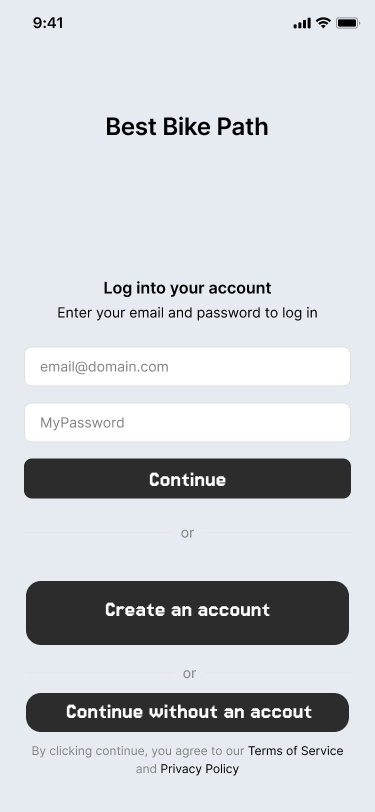
\includegraphics[width=0.4\linewidth]{RASD/Version1.0/images/Interfaces/Sign_In.png}
        \caption{Log in Interface} 
        \label{fig:log_in_interface}
    \end{center}
\end{figure}

Figure 3.1 represents the initial interface that any user encounters upon opening the application. From this screen, the user may choose to log in, sign up, or continue without creating an account, accessing a limited set of functionalities. 

\begin{figure}[H]
    \begin{center}
        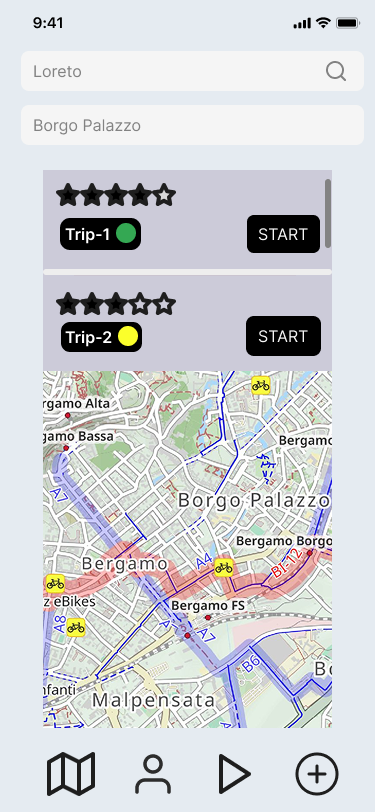
\includegraphics[width=0.4\linewidth]{RASD/Version1.0/images/Interfaces/Map_1.png}
        \caption{Map Interface} 
        \label{fig:Map_interface}
    \end{center}
\end{figure}

Figure 3.2 shows the map interface, which is displayed immediately after signing in or by selecting the map icon in the bottom navigation bar. At the top of the screen, a search bar allows the user to specify an origin and a destination in order to look for suitable cycling paths. Just below it, the suggested paths are presented, where the stars indicate the overall score of each path and the colored circle on the left represents the quality of the road. The map provides an overview of the available routes and serves as the central entry point for consulting path information and exploring the surrounding area.

\begin{figure}[H]
    \begin{center}
        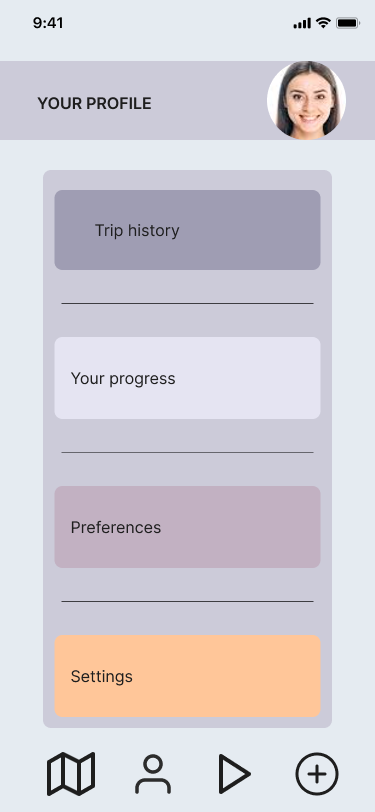
\includegraphics[width=0.4\linewidth]{RASD/Version1.0/images/Interfaces/Profile.png}
        \caption{Profile interface} 
        \label{fig:profile_interface}
    \end{center}
\end{figure}

Figure 3.3 illustrates the profile interface, which can be accessed by selecting the human-shaped icon in the bottom navigation bar. The \textit{Trip History} section displays all the user's completed trips and allows them to publish any unpublished paths as well as view detailed statistics for each ride. The \textit{Your Progress} section summarizes the user's overall activity, including metrics such as the total number of completed trips and the cumulative distance traveled. In the \textit{Preferences} section, the user can configure their preferred path qualities, enabling the system to provide personalized route suggestions. Finally, the \textit{Settings} section allows the user to modify their account information, such as changing their profile picture or deleting their account.

\begin{figure}[H]
    \begin{center}
        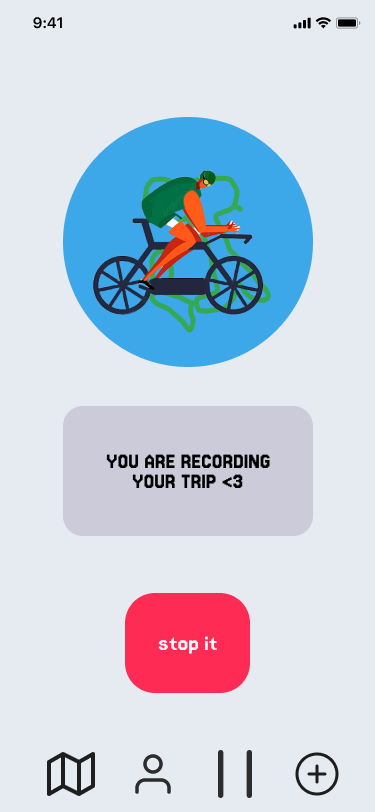
\includegraphics[width=0.4\linewidth]{RASD/Version1.0/images/Interfaces/Automatic 1.png}
        \caption{Automatic trip interface} 
        \label{fig:automatic_interface}
    \end{center}
\end{figure}

Figure 3.4 shows the interface displayed after pressing the start button in the bottom navigation bar, which initiates the automatic trip detection mode. During this mode, the system records the user's movement and collects sensor data to reconstruct the traveled path. The trip can be terminated at any time either by pressing the \textit{Stop} button on the screen or by selecting the same bottom navigation button, which now functions as a stop control. While the trip is being recorded, the user may continue to navigate and use the application freely without interrupting the ongoing detection process.

\begin{figure}[H]
    \begin{center}
        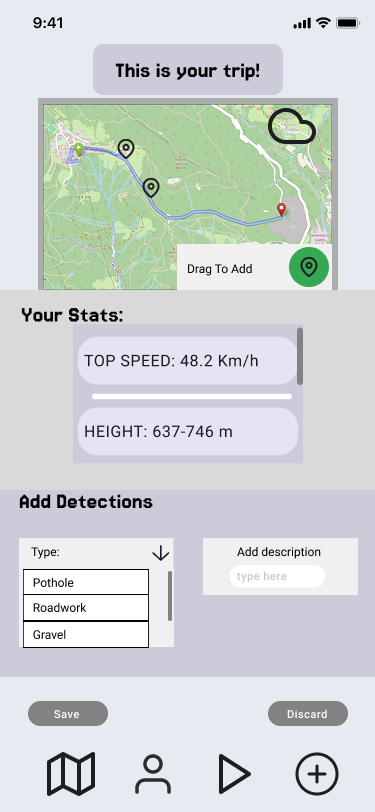
\includegraphics[width=0.4\linewidth]{RASD/Version1.0/images/Interfaces/Automatic 2.png}
        \caption{Detection confirmation interface} 
        \label{fig:automatic_detection}
    \end{center}
\end{figure}

Figure 3.5 shows the interface displayed after stopping the automatic trip detection illustrated in Figure 3.4. In this screen, the user can review the statistics of the completed trip and examine the automatically detected events. The lower section allows the user to add new detections or modify the ones suggested by the system. To precisely indicate where a detection occurred, the user can drag the pin on the map, positioning it on the exact road segment where the event took place.

\begin{figure}[H]
    \begin{center}
        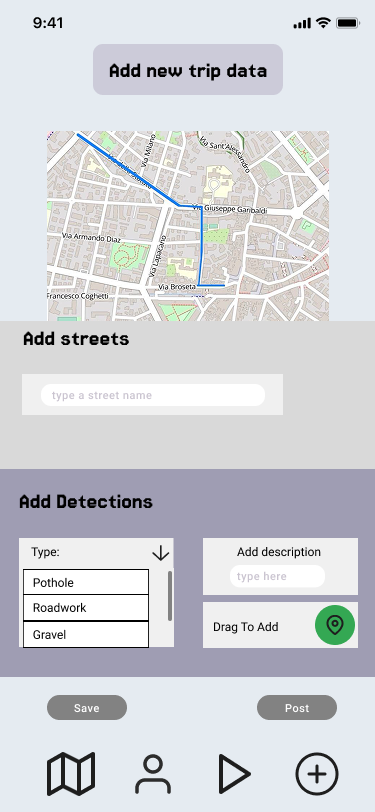
\includegraphics[width=0.4\linewidth]{RASD/Version1.0/images/Interfaces/Manual 1.png}
        \caption{Manual trip interface} 
        \label{fig:manual_interface}
    \end{center}
\end{figure}

Figure 3.6 can be accessed by pressing the ``+'' icon in the bottom navigation bar, allowing the user to create a trip manually. In this interface, the user may build a route by entering the names of the streets or by selecting their beginning and end points by clicking directly on the map and choosing an existing path between the two points. The blue lines represent the selected street segments. Once the route has been created, the user may continue forward to add the detections by pressing the \textit{Confirm path} button. In the following screen after having added the desired detections the user has the ability to either save the trip in his history or to directly post it as a contribution without saving it in his account.


\subsection{Hardware Interfaces}

The system shall ensure full compatibility with the hardware components involved in the interaction between users' devices and the platform. The following requirements apply:

\subsubsection*{User Devices}
\begin{itemize}
    \item The platform shall support access from a wide range of commonly used device such as tablets and smartphones. %mi sembra follia mettere anche tablet ma mi sembrava restrittivo dire solo smartphones 
    
    \item The platform shall be fully usable across different screen sizes and resolutions, ensuring responsiveness and readability regardless of device type.

    \item User devices shall include sufficient storage and processing capabilities to run the mobile application, including support for caching data and executing client-side scripts.

    \item For devices using automatic trip detection or sensor-based functionalities, the system shall interface with hardware components such as \textbf{GPS receivers}, \textbf{accelerometers}, and \textbf{gyroscopes}. These components must be accessible to the application for acquiring motion data, trip-related information, and geolocation.% non so se ha più senso in software o in hardware ma non metterei in entrambi
    
\end{itemize}


\subsection{Software Interfaces}

The system is designed as a mobile application, capable of performing all its core functionalities without relying on essential third-party software. Nevertheless, the system shall comply with the following software interface requirements:

\begin{itemize}
    \item The system shall function correctly across the most widely adopted operating systems, such as \textbf{Android}, and \textbf{iOS}.
    
    \item The system shall interface with geolocation and mapping services to retrieve, compute, and display cycling routes. These services include GPS modules, map-rendering libraries, and geocoding/route-search components.
    
    \item The system shall interface with external meteorological information providers to retrieve weather conditions relevant to trips and route safety evaluations and with external map service providers to retrieve geographical data.
    
    \item The system shall interact with mobile device sensors, including accelerometer and gyroscope, to collect motion-related data supporting the automatic detection of obstacles and road conditions.
    
    \item No additional software installations or configurations shall be required on the user's device, aside from using the official mobile application.
\end{itemize}

\subsection{Communication Interfaces}

The system shall support reliable and secure communication mechanisms enabling interaction between client devices, backend services, and external data providers. The following requirements apply:

\begin{itemize}
    \item The system shall operate over standard Internet connections, such as \textbf{Wi-Fi}, and \textbf{mobile data}.
    
    \item All communication between the client and the server shall be secured through \textbf{encrypted protocols} (e.g., TLS/SSL) to protect sensitive information such as user credentials, personal data, recorded trips, and sensor-based contributions.
    
    \item The system shall utilize widely adopted \textbf{web communication protocols}, primarily \textbf{HTTPS}, to ensure secure and reliable data transmission between user devices and the backend.
    
    \item The system shall support communication with external services, including meteorological data providers and geolocation/map services, through standard \textbf{HTTP/HTTPS-based APIs}.
    
    \item No additional software installations or communication packages shall be required on the user’s device to enable proper communication with the platform.
    
    \item The system shall minimize communication latency by adhering to industry-standard response times ensuring a smooth and responsive user experience.
\end{itemize}


\subsubsection*{Hosting Infrastructure}
\begin{itemize}
    \item The system shall be deployed on a hosting infrastructure capable of supporting simultaneous access by multiple users with minimal latency.
    
    \item The hosting environment shall provide sufficient computational resources for processing real-time map data, aggregating user contributions, and executing background operations.

    \item The infrastructure shall include adequate storage capabilities to manage user profiles, trips, sensor data, and historical records of contributions.

    \item The hosting environment shall be scalable, allowing the system to accommodate increasing traffic, data volume, and computational demands over time while preserving service availability and performance.
\end{itemize}



\section{Functional Requirements}
\label{sec:functional_requirements}

\begin{figure}[H]
    \begin{center}
        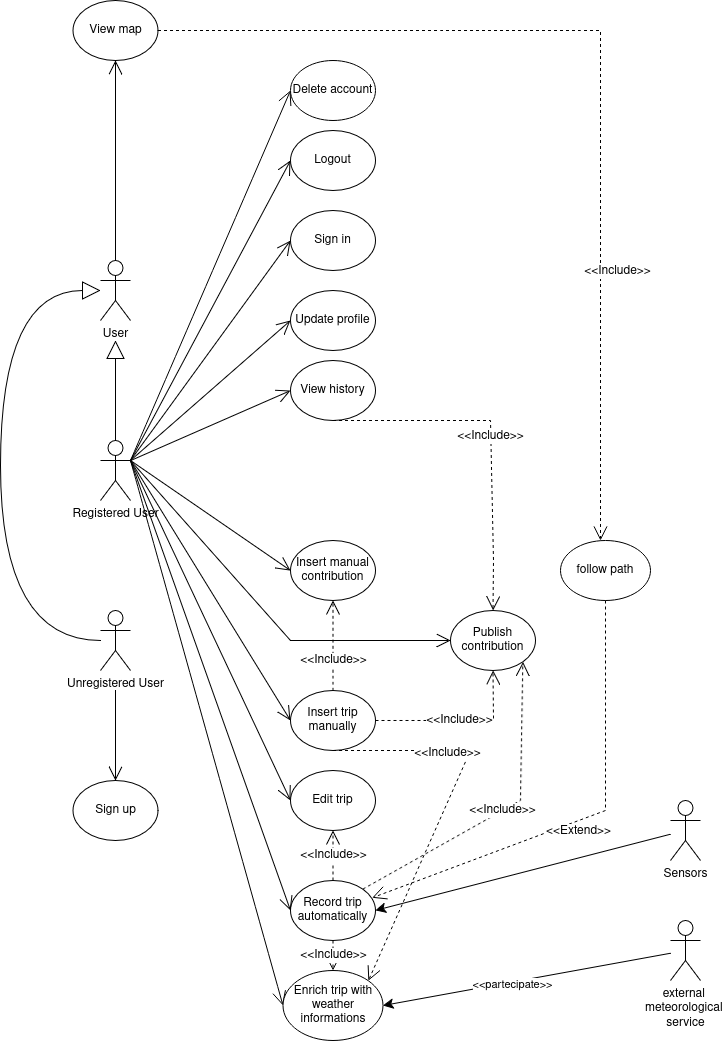
\includegraphics[width=0.9\linewidth]{RASD/Version1.0/images/use_case_diagram.png}
        \caption{Use Case Diagram} 
        \label{fig:use_case_diagram}
    \end{center}
\end{figure}

\newpage
\subsection{Use Cases and Activity Diagrams}
\label{subsec: use_cases}%

\newcounter{ucsteps}
\setcounter{ucsteps}{1}
\newcommand{\cucsteps}{\theucsteps\stepcounter{ucsteps}}
\newcommand{\resetucsteps}{\setcounter{ucsteps}{1}}

\newcounter{uc}
\setcounter{uc}{1}
\newcommand{\cuc}{\theuc\stepcounter{uc}\resetucsteps}

\subsubsection*{UC\cuc . Sign Up}
\begin{center}
    \begin{longtable}{|l|p{0.75\linewidth}|}
        \hline
        \textbf{Actor}            & User\\
        \hline
        \textbf{Entry Conditions} & The User is not logged into the platform and is on the homepage. \\
        \hline
        \textbf{Flow of Events}    
        & \cucsteps. On the homepage, the User clicks the ``Sign up'' button. \\
        & \cucsteps. The system displays the registration form. \\
        & \cucsteps. The User inserts the required registration details (e.g., email, password and password confirmation). \\
        & \cucsteps. The User confirms the provided information by clicking the ``Register'' button. \\
        & \cucsteps. The system checks the completeness and validity of the submitted data. \\
        & \cucsteps. If the data is valid, the system sends a confirmation email containing a verification link that expires after 24 hours. \\
        & \cucsteps. The User clicks the confirmation link in the email before it expires. \\
        & \cucsteps. The system allows the User to access the profile page and complete the profile by inserting the remaining personal details. \\
        \hline
        \textbf{Exit Conditions}   & The User account is created and verified, and the profile is completed so that the User can access the platform functionalities.\\       
        \hline
        \textbf{Exceptions}       & \begin{itemize}[leftmargin=*]
            \item Some mandatory fields are missing: the system notifies ``Missing mandatory fields'' and does not allow the User to proceed until all required fields are filled in.
            \item The password does not satisfy the platform's security requirements: the system notifies ``Invalid password'' and prompts the User to correct it.
            \item The email address is already linked to an existing account: the system notifies ``Email already linked'' and redirects the User to the login page.
            \item The confirmation link expires before being used: the system discards all data previously inserted by the User and invalidates the link.
        \end{itemize} \\
        \hline
    \end{longtable}
\end{center}


\begin{figure}[H]
    \begin{center}
         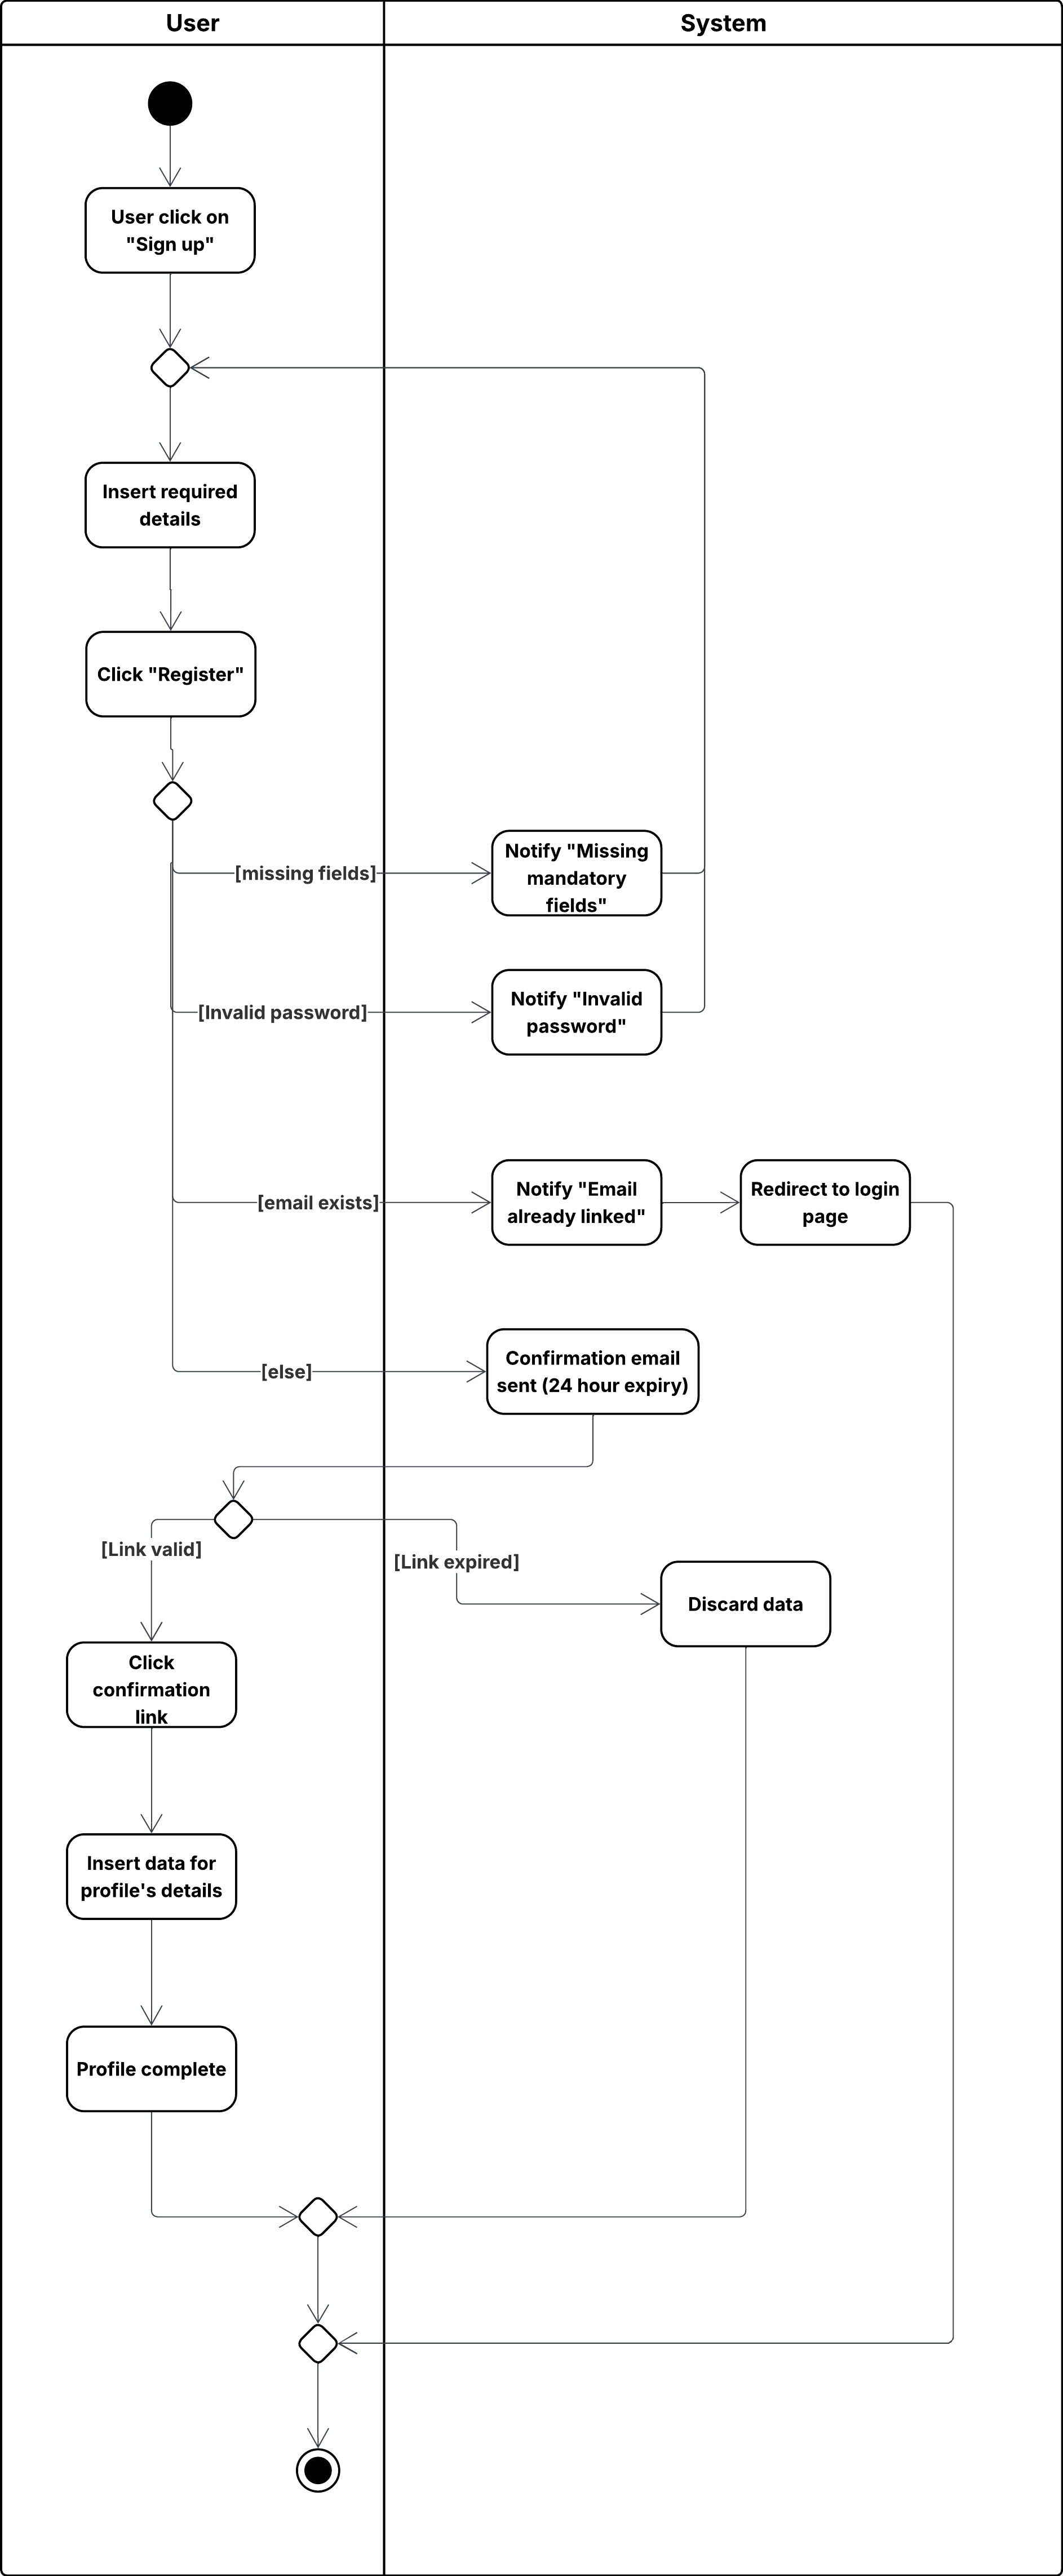
\includegraphics[width=0.5\linewidth]{RASD/Version1.0/images/activity diagram/UC1.png}
         \caption{Sign Up}
         \label{fig:signup_student_ad}
     \end{center}
\end{figure}

\newpage


\subsubsection*{UC\cuc . Sign In}
\begin{center}
    \begin{longtable}{|l|p{0.75\linewidth}|}
        \hline
        \textbf{Actor}            & User \\
        \hline
        \textbf{Entry Conditions} & The User is not logged into the platform and is on the homepage. \\
        \hline
        \textbf{Flow of Events}    
        & \cucsteps. On the homepage, the User clicks the ``Sign in'' button. \\
        & \cucsteps. The system displays the login form. \\
        & \cucsteps. The User enters their credentials (email and password). \\
        & \cucsteps. The User clicks the ``Login'' button to submit the credentials. \\
        & \cucsteps. The system validates the provided credentials. \\
        & \cucsteps. If the credentials are valid and the account is verified, the system checks whether the User's profile is complete. \\
        & \cucsteps. If the profile is complete, the system redirects the User to the Home page. \\
        & \cucsteps. If the profile is not complete, the system redirects the User to the ``Update profile'' page. \\
        \hline
        \textbf{Exit Conditions}   & The User is successfully authenticated and is redirected either to the Home page or to the profile completion page.\\
        \hline
        \textbf{Exceptions}       & {%
            \begin{itemize}[leftmargin=*]
                \item The entered credentials are not valid: the system notifies ``Entered credentials are not valid'' and does not log the User in.
                \item The account associated with the provided email is not verified: the system notifies ``Account not verified'' and does not log the User in.
            \end{itemize}
        } \\
        \hline
    \end{longtable}
\end{center}



\begin{figure}[H]
    \begin{center}
         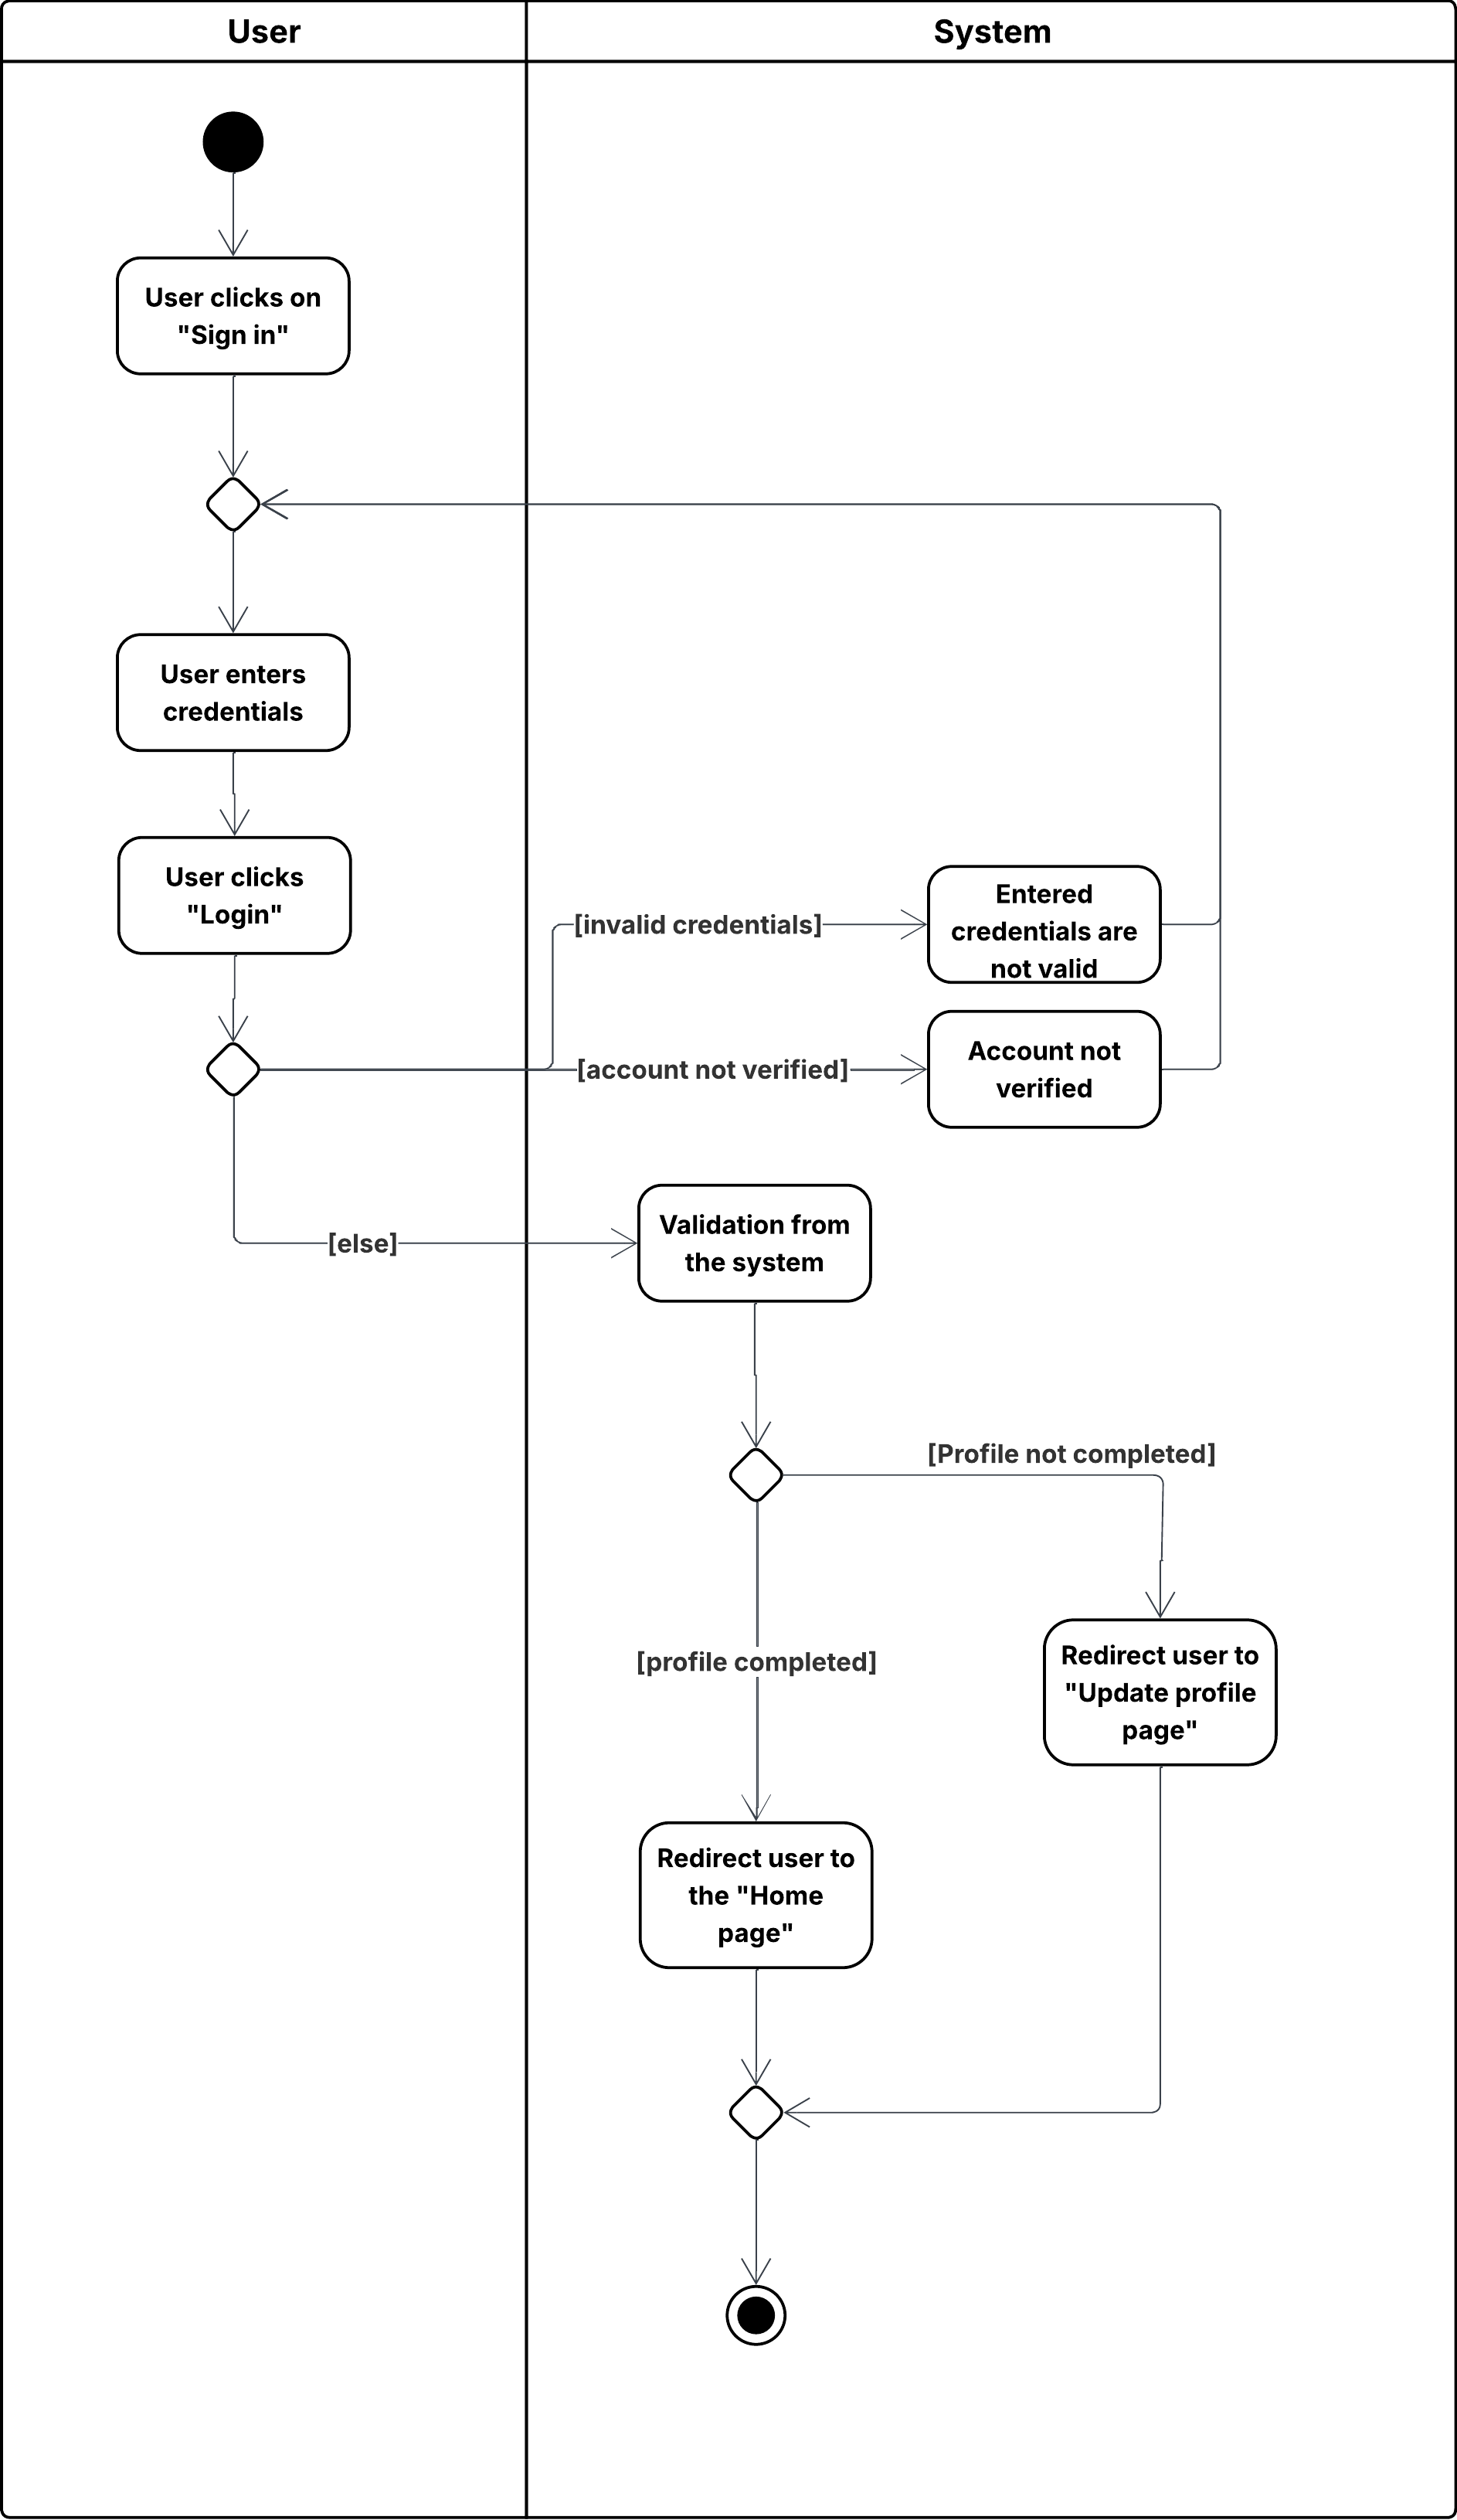
\includegraphics[width=0.5\linewidth]{RASD/Version1.0/images/activity diagram/UC2.png}
         \caption{Sign In}
         \label{fig:signin}
     \end{center}
\end{figure}

\newpage


\subsubsection*{UC\cuc . Delete Account}
\begin{center}
    \begin{longtable}{|l|p{0.75\linewidth}|}
        \hline
        \textbf{Actor}            & Registered User \\
        \hline
        \textbf{Entry Conditions} & The Registered User is logged into the platform and is on the account settings page. \\
        \hline
        \textbf{Flow of Events}    
        & \cucsteps. The User opens the account settings section. \\
        & \cucsteps. The User selects the ``Delete account'' option. \\
        & \cucsteps. The system shows a warning explaining the consequences of account deletion and asks the User whether they want to continue. \\
        & \cucsteps. The User confirms the intention to proceed with account deletion. \\
        & \cucsteps. The system requests re-authentication by asking the User to enter their credentials. \\
        & \cucsteps. The User inserts their credentials and submits them. \\
        & \cucsteps. The system validates the provided credentials. \\
        & \cucsteps. If the credentials are valid, the system removes the User profile and related personal information. \\
        & \cucsteps. The system deletes the trips stored for the User. \\
        & \cucsteps. The system deletes the User's preferences and local settings. \\
        & \cucsteps. The system invalidates any active sessions and authentication tokens associated with the User. \\
        & \cucsteps. The system notifies the User that the account has been successfully deleted. \\
        \hline
        \textbf{Exit Conditions}   & The User account and all associated data are deleted, and the User is no longer able to access the platform with the previous credentials.\\
        \hline
        \textbf{Exceptions}       & {%
            \begin{itemize}[leftmargin=*]
                \item The User cancels the deletion after viewing the warning: the system returns the User to the account settings page without performing any deletion.
                \item The re-authentication credentials are not valid: the system notifies the User that the credentials are invalid and returns to the account settings page without deleting the account.
            \end{itemize}
        } \\
        \hline
    \end{longtable}
\end{center}


\begin{figure}[H]
    \begin{center}
         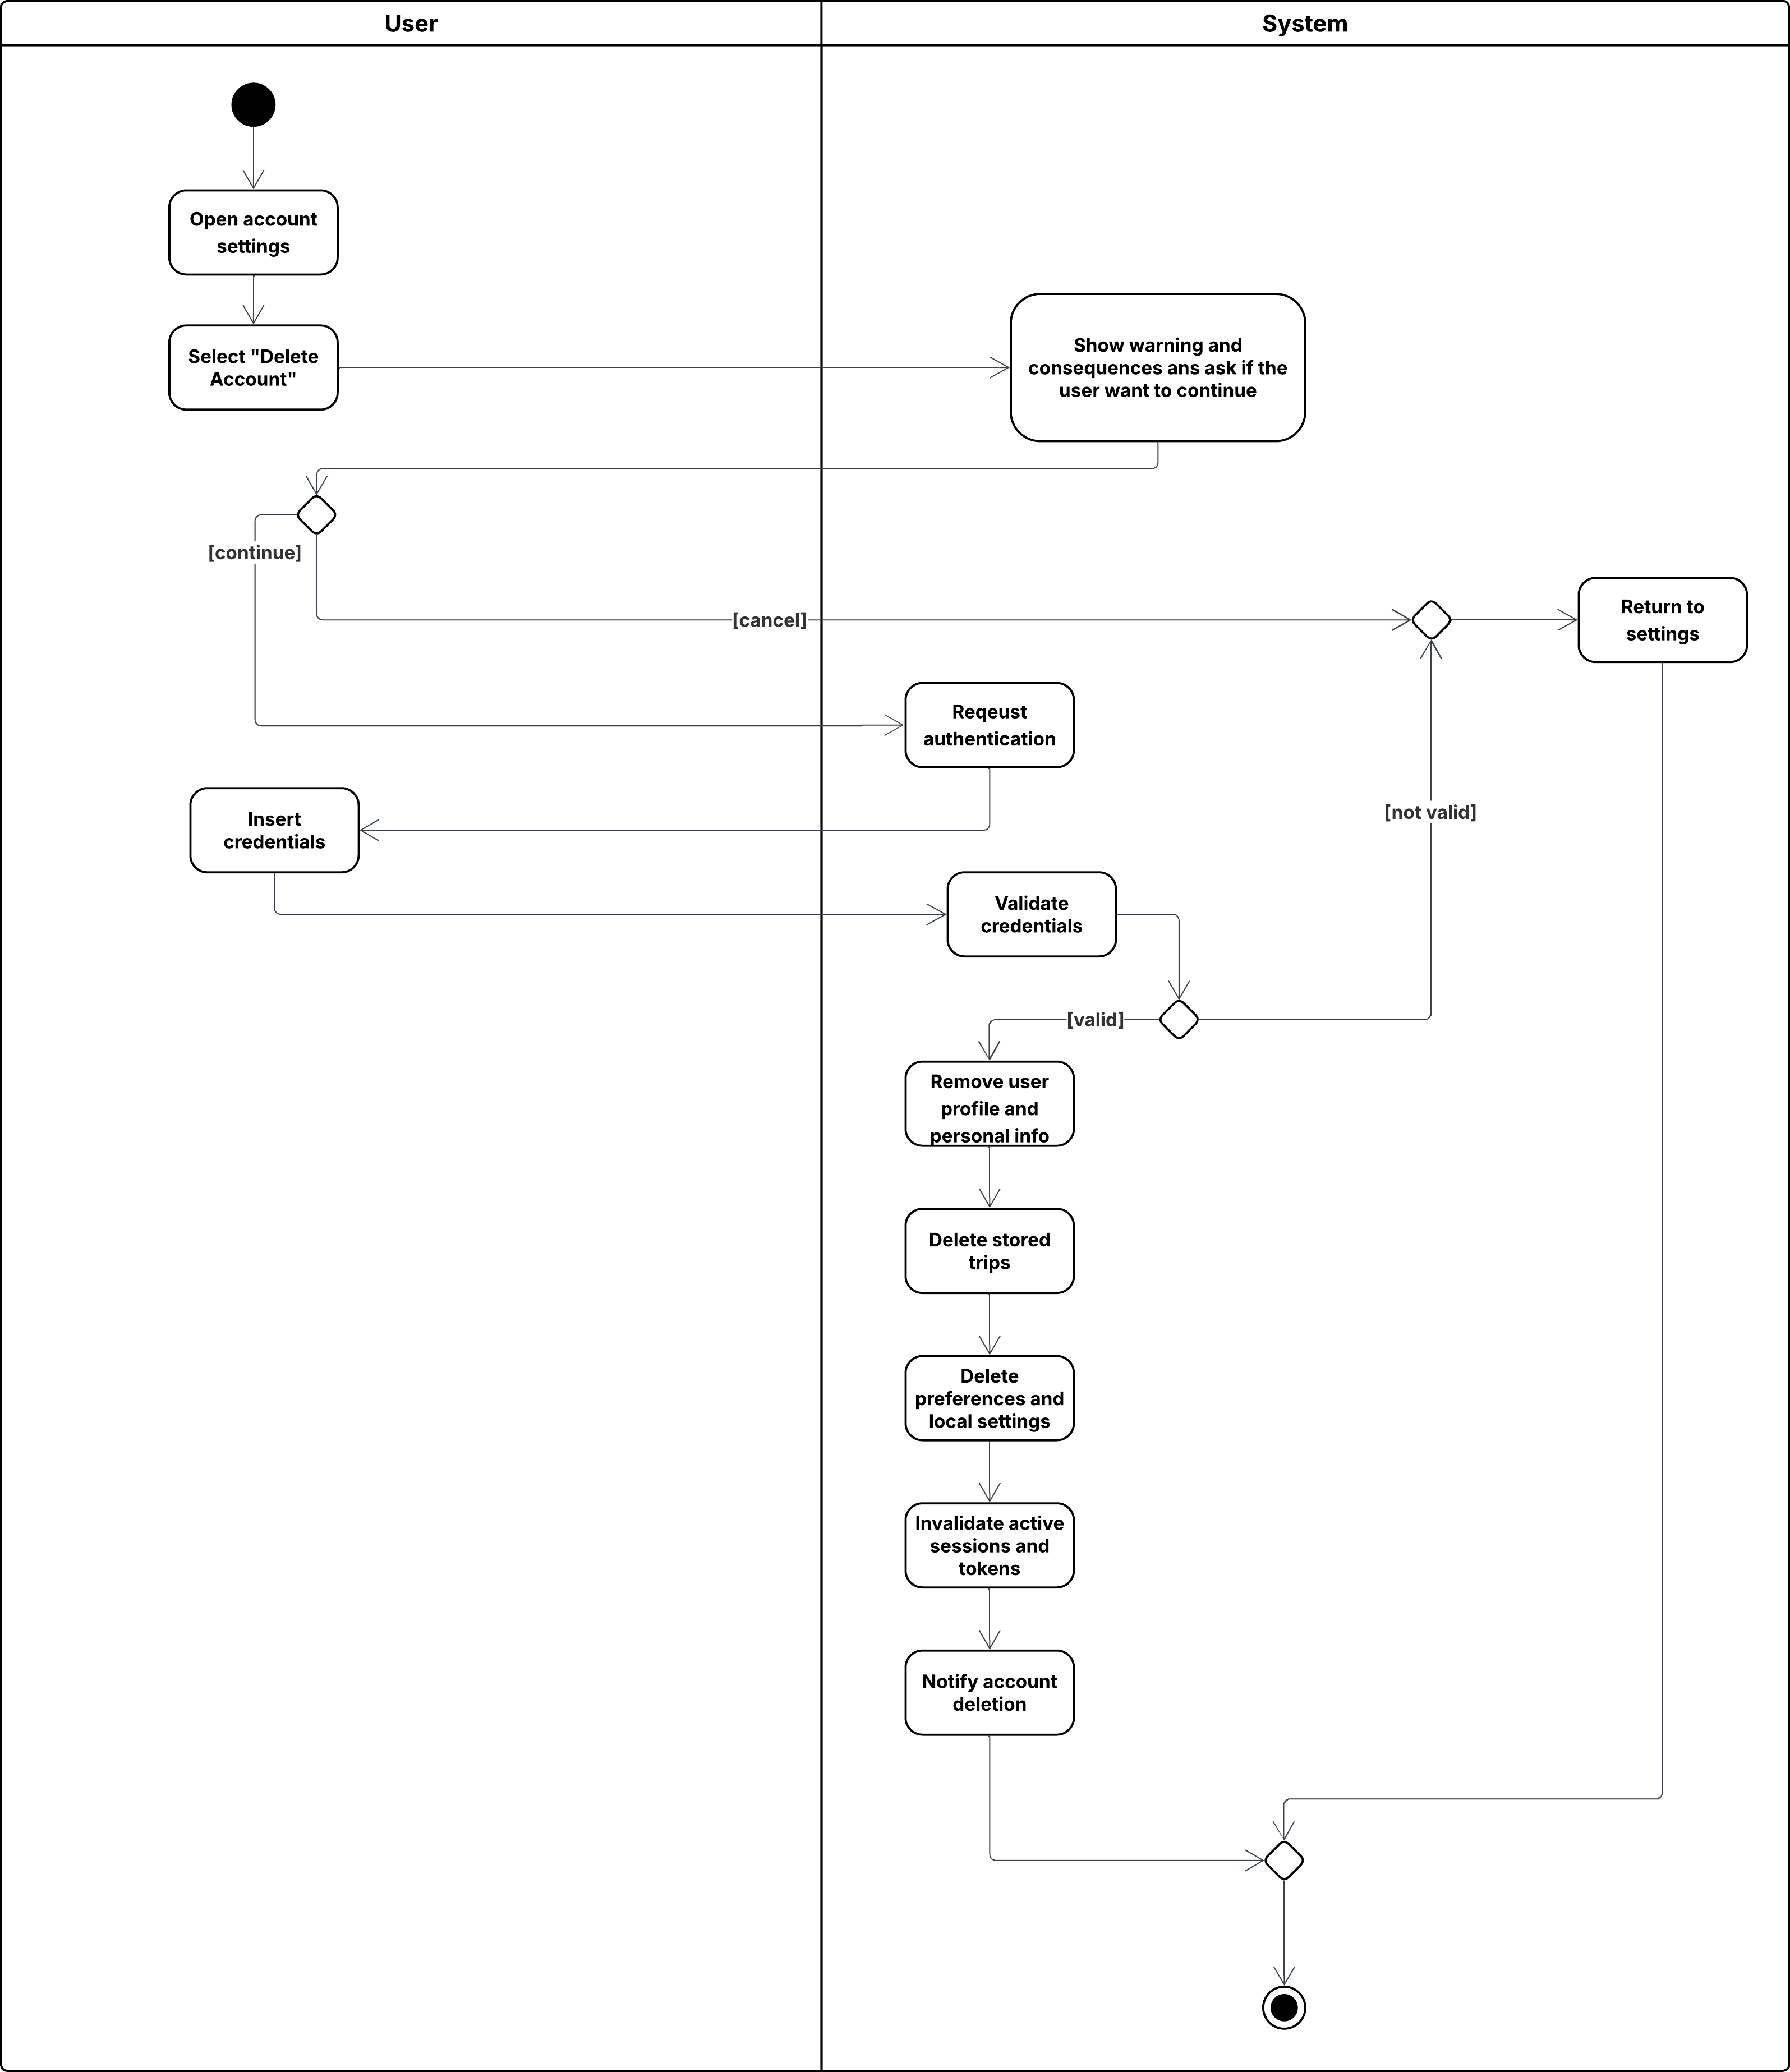
\includegraphics[width=0.9\linewidth]{RASD/Version1.0/images/activity diagram/UC3.png}
         \caption{Delete Account}
         \label{fig:delete_account}
     \end{center}
\end{figure}

\newpage


\subsubsection*{UC\cuc . Logout}
\begin{center}
    \begin{longtable}{|l|p{0.75\linewidth}|}
        \hline
        \textbf{Actor}            & User \\
        \hline
        \textbf{Entry Conditions} & The User is logged into the platform. \\
        \hline
        \textbf{Flow of Events}    
        & \cucsteps. The User clicks on the ``Logout'' button. \\
        & \cucsteps. The system receives the logout request. \\
        & \cucsteps. The system terminates the User's session and invalidates any active authentication token. \\
        & \cucsteps. The system redirects the User to the Home screen. \\
        \hline
        \textbf{Exit Conditions}   & The User's session is terminated, and the User is no longer authenticated on the platform.\\
        \hline
        \textbf{Exceptions}       & {%
            \begin{itemize}[leftmargin=*]
                \item None.
            \end{itemize}
        } \\
        \hline
    \end{longtable}
\end{center}




\begin{figure}[H]
    \begin{center}
         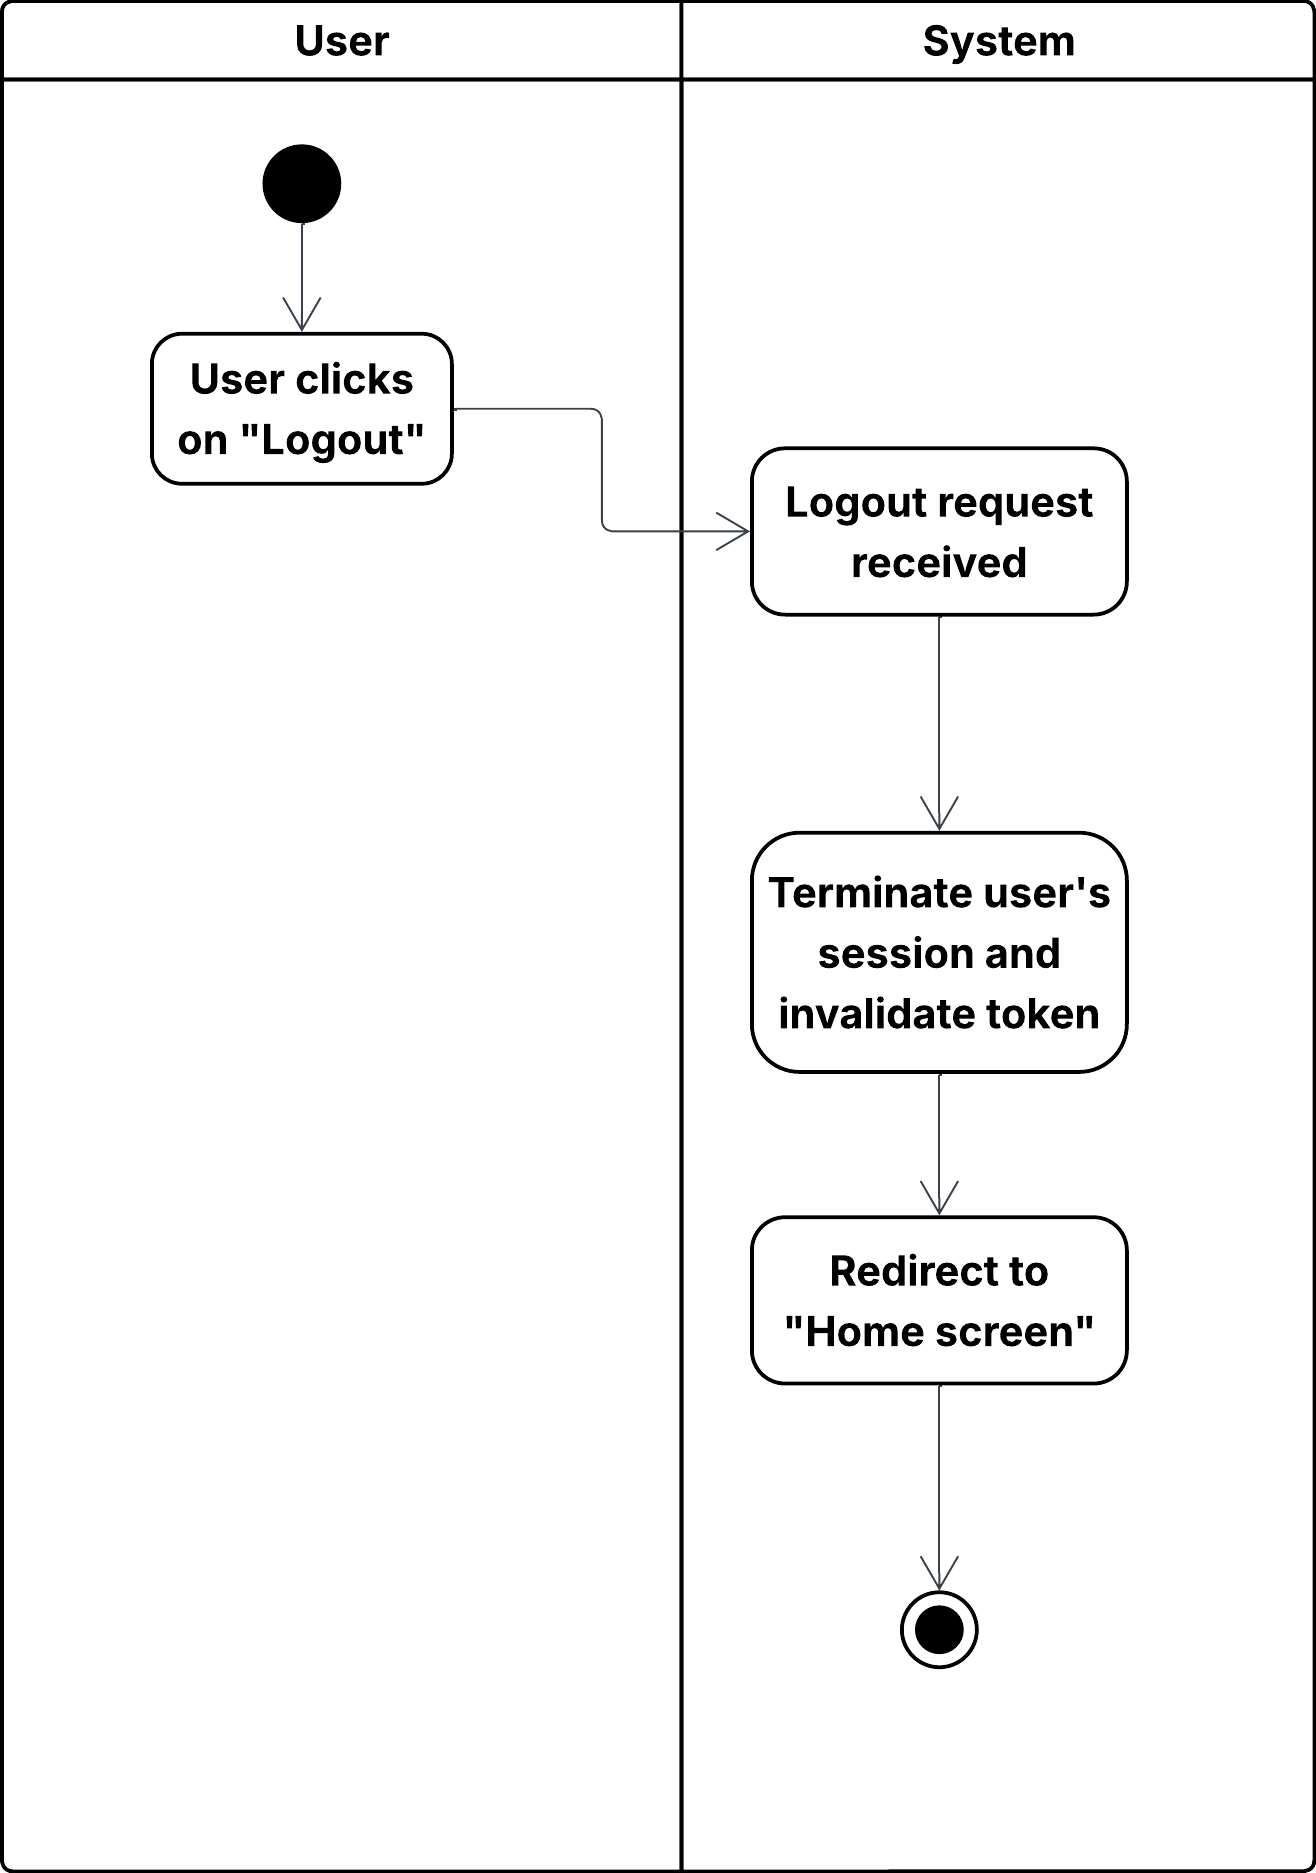
\includegraphics[width=0.9\linewidth]{RASD/Version1.0/images/activity diagram/UC4.png}
         \caption{Logout}
         \label{fig:Logout}
     \end{center}
\end{figure}

\newpage

\subsubsection*{UC\cuc . Edit Profile}
\begin{center}
    \begin{longtable}{|l|p{0.75\linewidth}|}
        \hline
        \textbf{Actor}            & Registered User \\
        \hline
        \textbf{Entry Conditions} & The Registered User is logged into the platform. \\
        \hline
        \textbf{Flow of Events}    
        & \cucsteps. The User clicks on the ``Profile'' section. \\
        & \cucsteps. The User clicks on the ``Edit profile'' option inside the settings. \\
        & \cucsteps. The system displays the editable profile form, including personal data and preference fields. \\
        & \cucsteps. The User updates the desired information, such as personal details and visualization preferences (e.g., preferred path filters based on past trips). \\
        & \cucsteps. The User clicks the ``Apply'' button to confirm the changes. \\
        & \cucsteps. The system validates the submitted changes. \\
        & \cucsteps. If the changes are valid, the system stores them and notifies the User of the successful update. \\
        \hline
        \textbf{Exit Conditions}   & The User's profile and preferences are updated and consistently stored in the system.\\
        \hline
        \textbf{Exceptions}       & {%
            \begin{itemize}[leftmargin=*]
                \item Some updated fields are not valid (e.g., invalid email format or unsupported preference values): the system notifies the User that the changes are not valid and does not apply them.
            \end{itemize}
        } \\
        \hline
    \end{longtable}
\end{center}


\begin{figure}[H]
    \begin{center}
         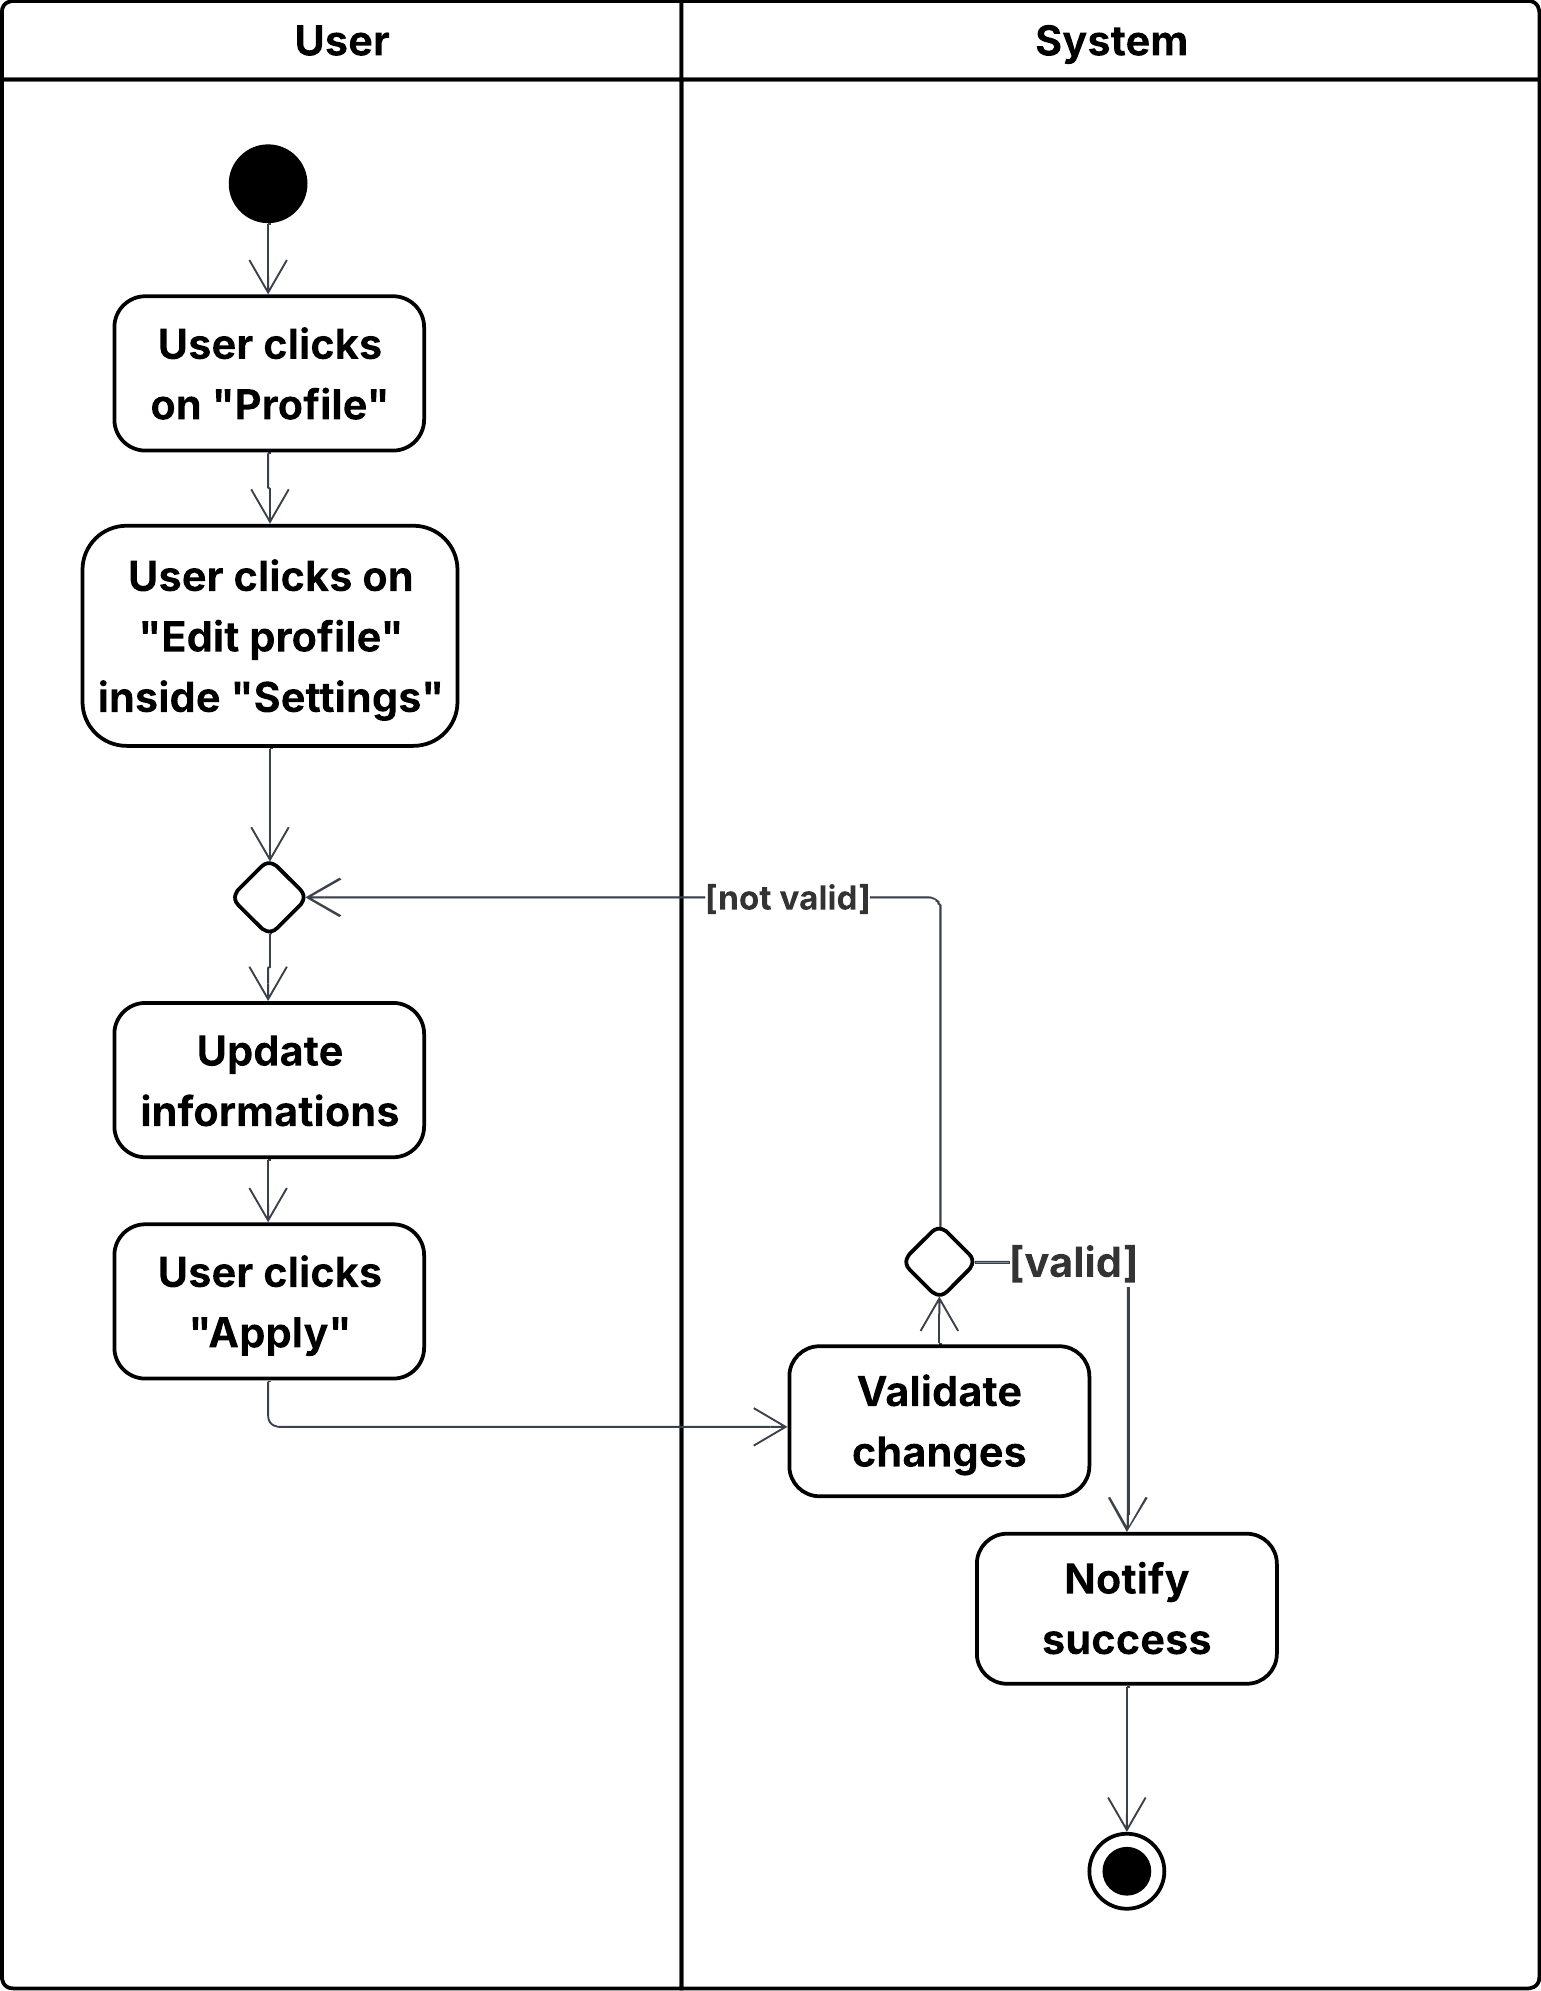
\includegraphics[width=0.9\linewidth]{RASD/Version1.0/images/activity diagram/UC5.png}
         \caption{Edit Profile}
         \label{fig:edit_profile}
     \end{center}
\end{figure}

\newpage

\subsubsection*{UC\cuc . View Trip History}
\begin{center}
    \begin{longtable}{|l|p{0.75\linewidth}|}
        \hline
        \textbf{Actor}            & Registered User \\
        \hline
        \textbf{Entry Conditions} & The Registered User is logged into the platform. \\
        \hline
        \textbf{Flow of Events}    
        & \cucsteps. The User clicks on the ``My trips'' section. \\
        & \cucsteps. The system retrieves the trips associated with the User and shows the list of available trips. \\
        & \cucsteps. The User selects one trip from the list. \\
        & \cucsteps. The system shows the selected trip together with its stored data and associated contributions. \\
        & \cucsteps. The User chooses an action for the selected trip (e.g., to publish its contributions or to simply inspect the data). \\
        & \cucsteps. If the User decides to publish the contributions of the trip, the system starts the \hyperref[sec:publish_contribution]{\uline{UC.~Publishing Contribution}} use case for the first contribution associated with that trip. \\
        & \cucsteps. The system iteratively processes the contributions linked to the trip, publishing them one at a time so that merge and update policies on paths can be correctly applied for each contribution. \\
        & \cucsteps. When there are no more contributions to process, the system returns control to the trip view. \\
        & \cucsteps. For readability, the activity diagram omits the fact that the User can navigate back to previous pages (trip list or other sections of the app) at any point in the interaction. \\
        \hline
        \textbf{Exit Conditions}   & The User has viewed the selected trip and, if desired, has published the contributions associated with that trip.\\
        \hline
        \textbf{Exceptions}       & {%
            \begin{itemize}[leftmargin=*]
                \item The User has no stored trips: the system shows an empty list and may display an informative message.
                \item The selected trip has no associated contributions: the system shows the trip data but does not start the publishing process.
            \end{itemize}
        } \\
        \hline
    \end{longtable}
\end{center}


\begin{figure}[H]
    \begin{center}
         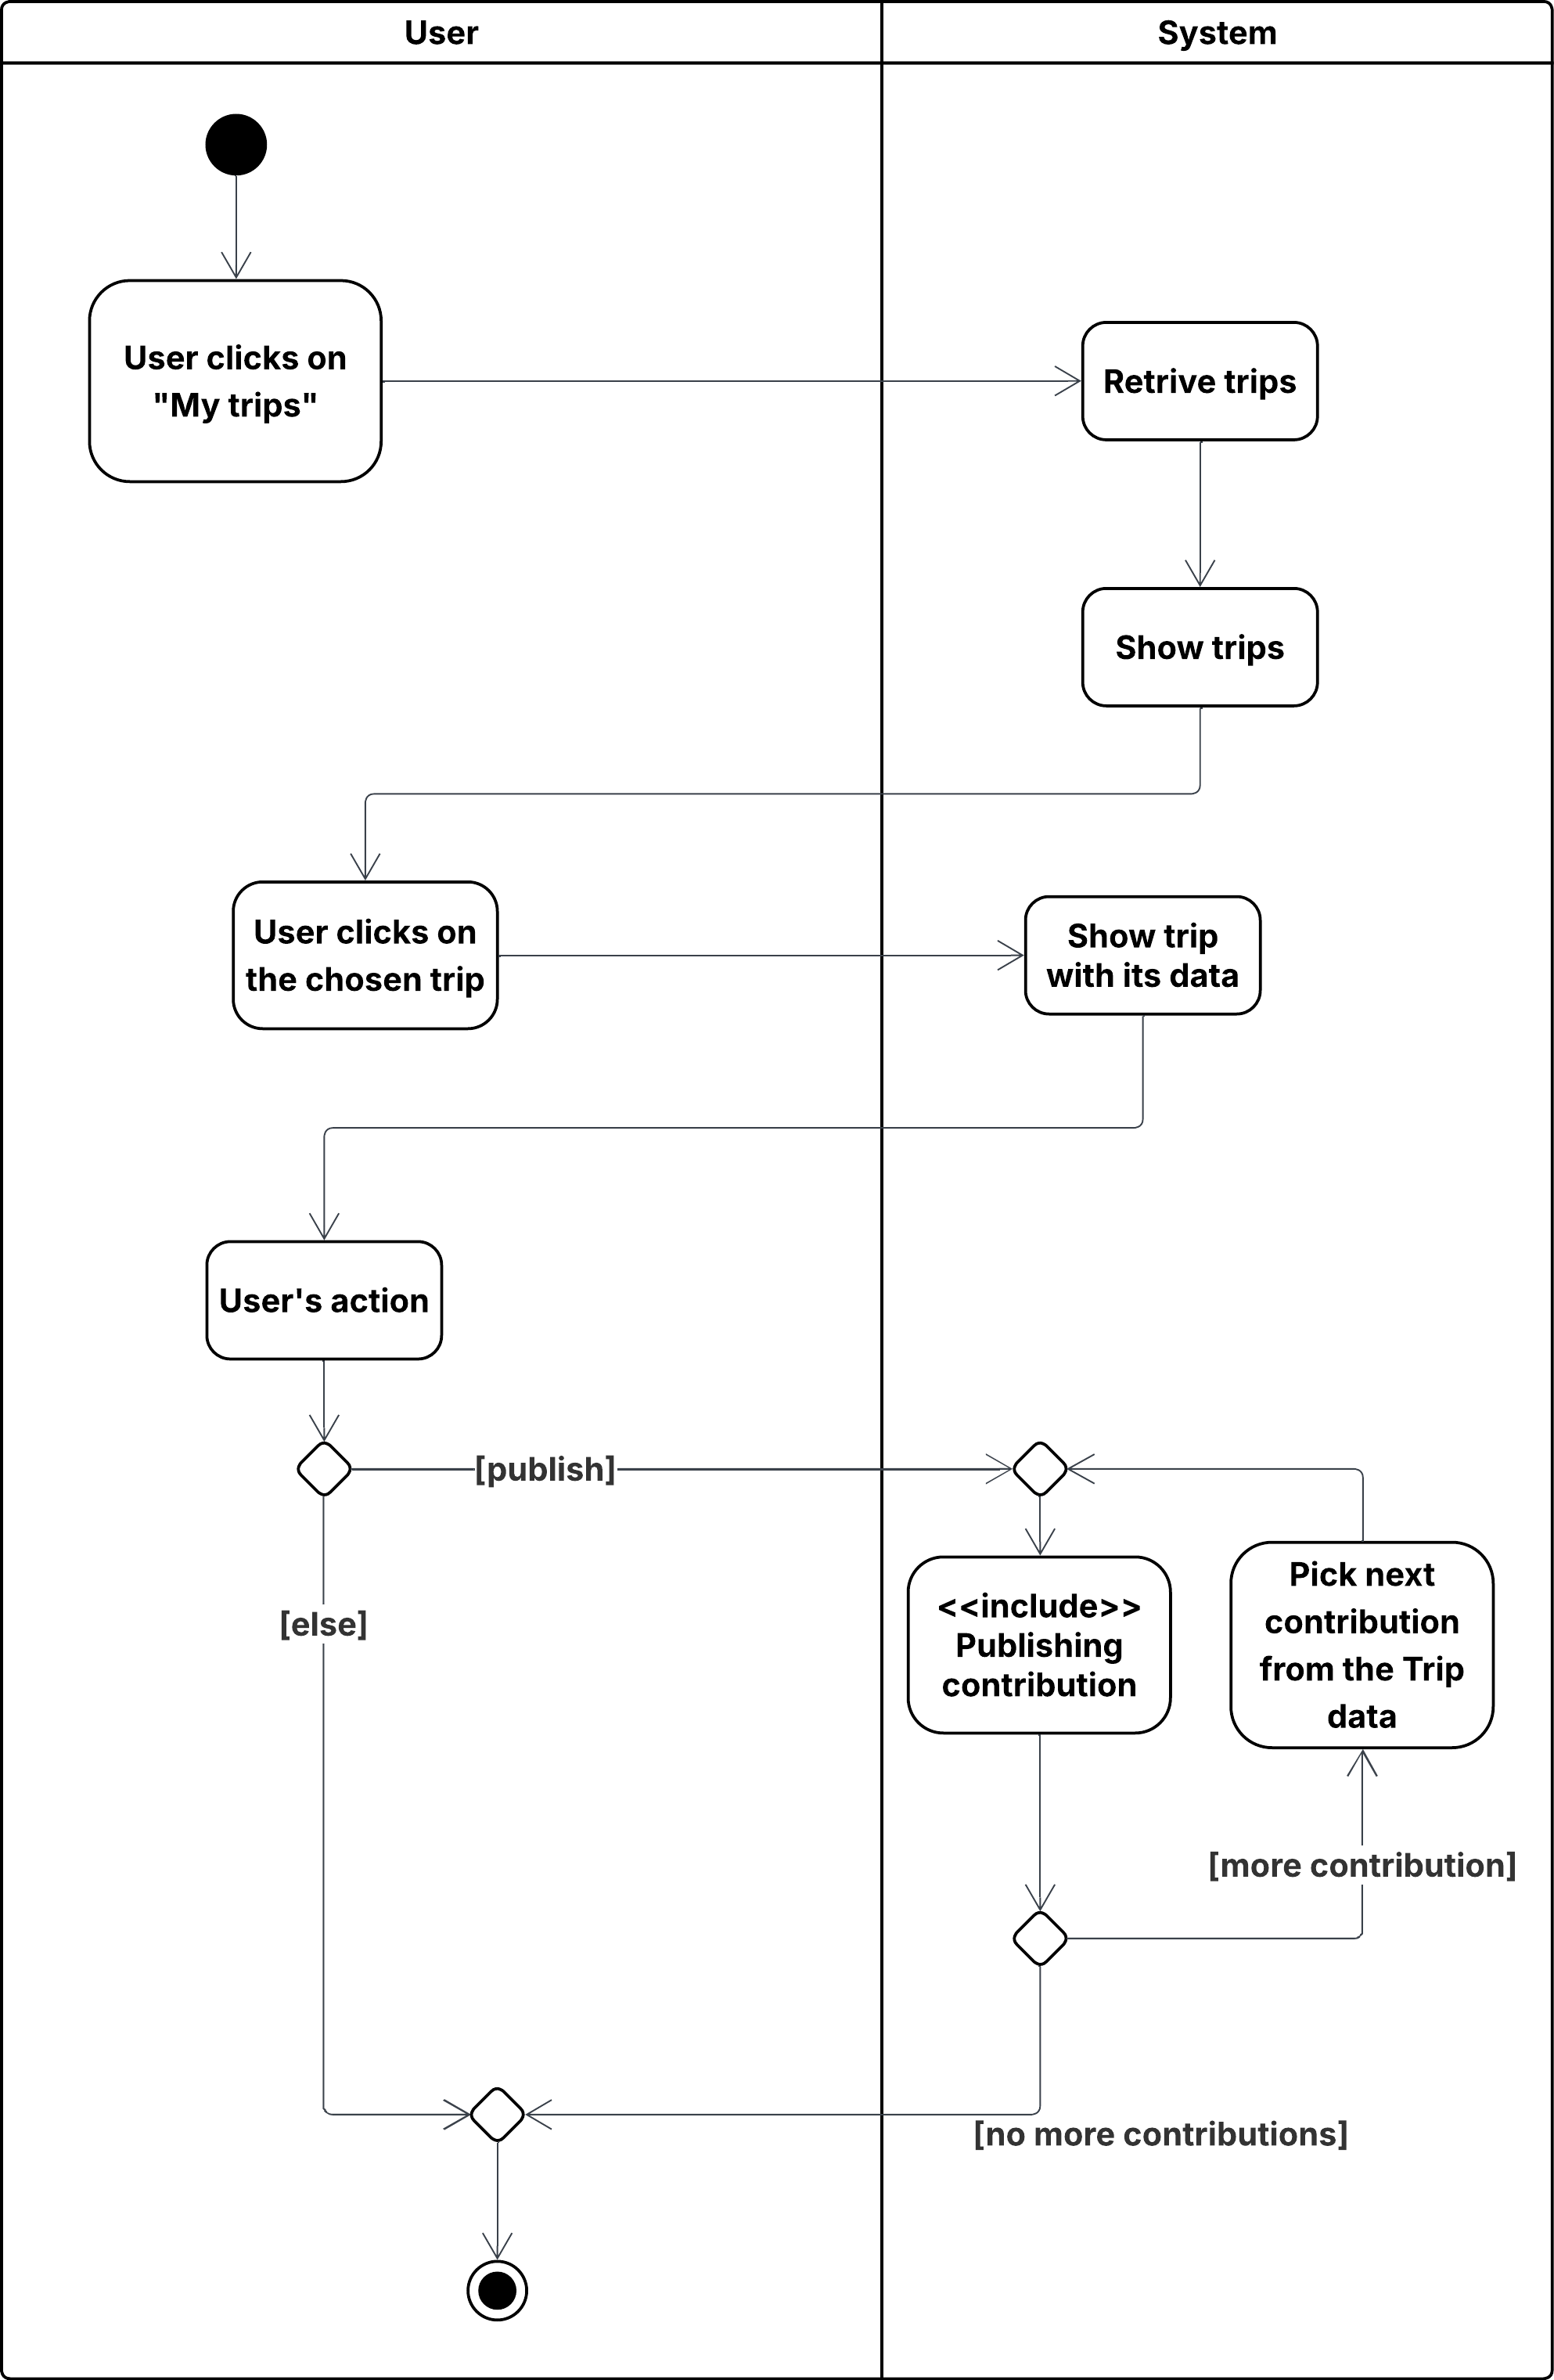
\includegraphics[width=0.9\linewidth]{RASD/Version1.0/images/activity diagram/UC6.png}
         \caption{View Trip History}
         \label{fig:view_trip_history}
     \end{center}
\end{figure}

\newpage




\subsubsection*{UC\cuc . Publish Contribution}
\label{sec:uc_publish_contribution}
\begin{center}
    \begin{longtable}{|l|p{0.75\linewidth}|}
        \hline
        \textbf{Actor}            & System (invoked from other use cases, e.g. View Trip History) \\
        \hline
        \textbf{Entry Conditions} & A Contribution has been selected for publication (for example, from a Trip in the User's history). \\
        \hline
        \textbf{Flow of Events}    
        & \cucsteps. The system validates the selected Contribution, checking that its data is complete and consistent. \\
        & \cucsteps. If the Contribution is valid, the system retrieves from the database any existing Contribution(s) referring to the same street or path segment. \\
        & \cucsteps. The system applies the configured merging policy to combine the new Contribution with the existing information (e.g., updating or aggregating obstacle data on that path). \\
        & \cucsteps. The system updates the corresponding path information in the database according to the result of the merging policy. \\
        & \cucsteps. The system flags the User's Contribution as published. \\
        & \cucsteps. The system notifies the successful publication of the Contribution to the invoking use case. \\
        \hline
        \textbf{Exit Conditions}   & The Contribution is marked as published and the affected path information in the database has been updated according to the merging policy.\\
        \hline
        \textbf{Exceptions}       & {%
            \begin{itemize}[leftmargin=*]
                \item The Contribution is not valid (e.g., missing mandatory data or inconsistent location): the system notifies the failure and does not modify any existing path information.
                \item A database error occurs while retrieving or updating existing Contributions: the system notifies the failure and leaves the User's Contribution in a non-published state.
            \end{itemize}
        } \\
        \hline
    \end{longtable}
\end{center}

\paragraph{Important Note}
This use case describes the \emph{conceptual} behavior of the system from the perspective of the involved stakeholders.  
In particular, it does not reflect the actual implementation details of the publication process, which, as discussed in the Design Document, is realized through an asynchronous mechanism.  

The use case abstracts away such implementation aspects and focuses instead on what should logically occur and on what the registered user is expected to perceive in terms of system behavior and outcomes, regardless of the underlying execution model.


\begin{figure}[H]
    \begin{center}
         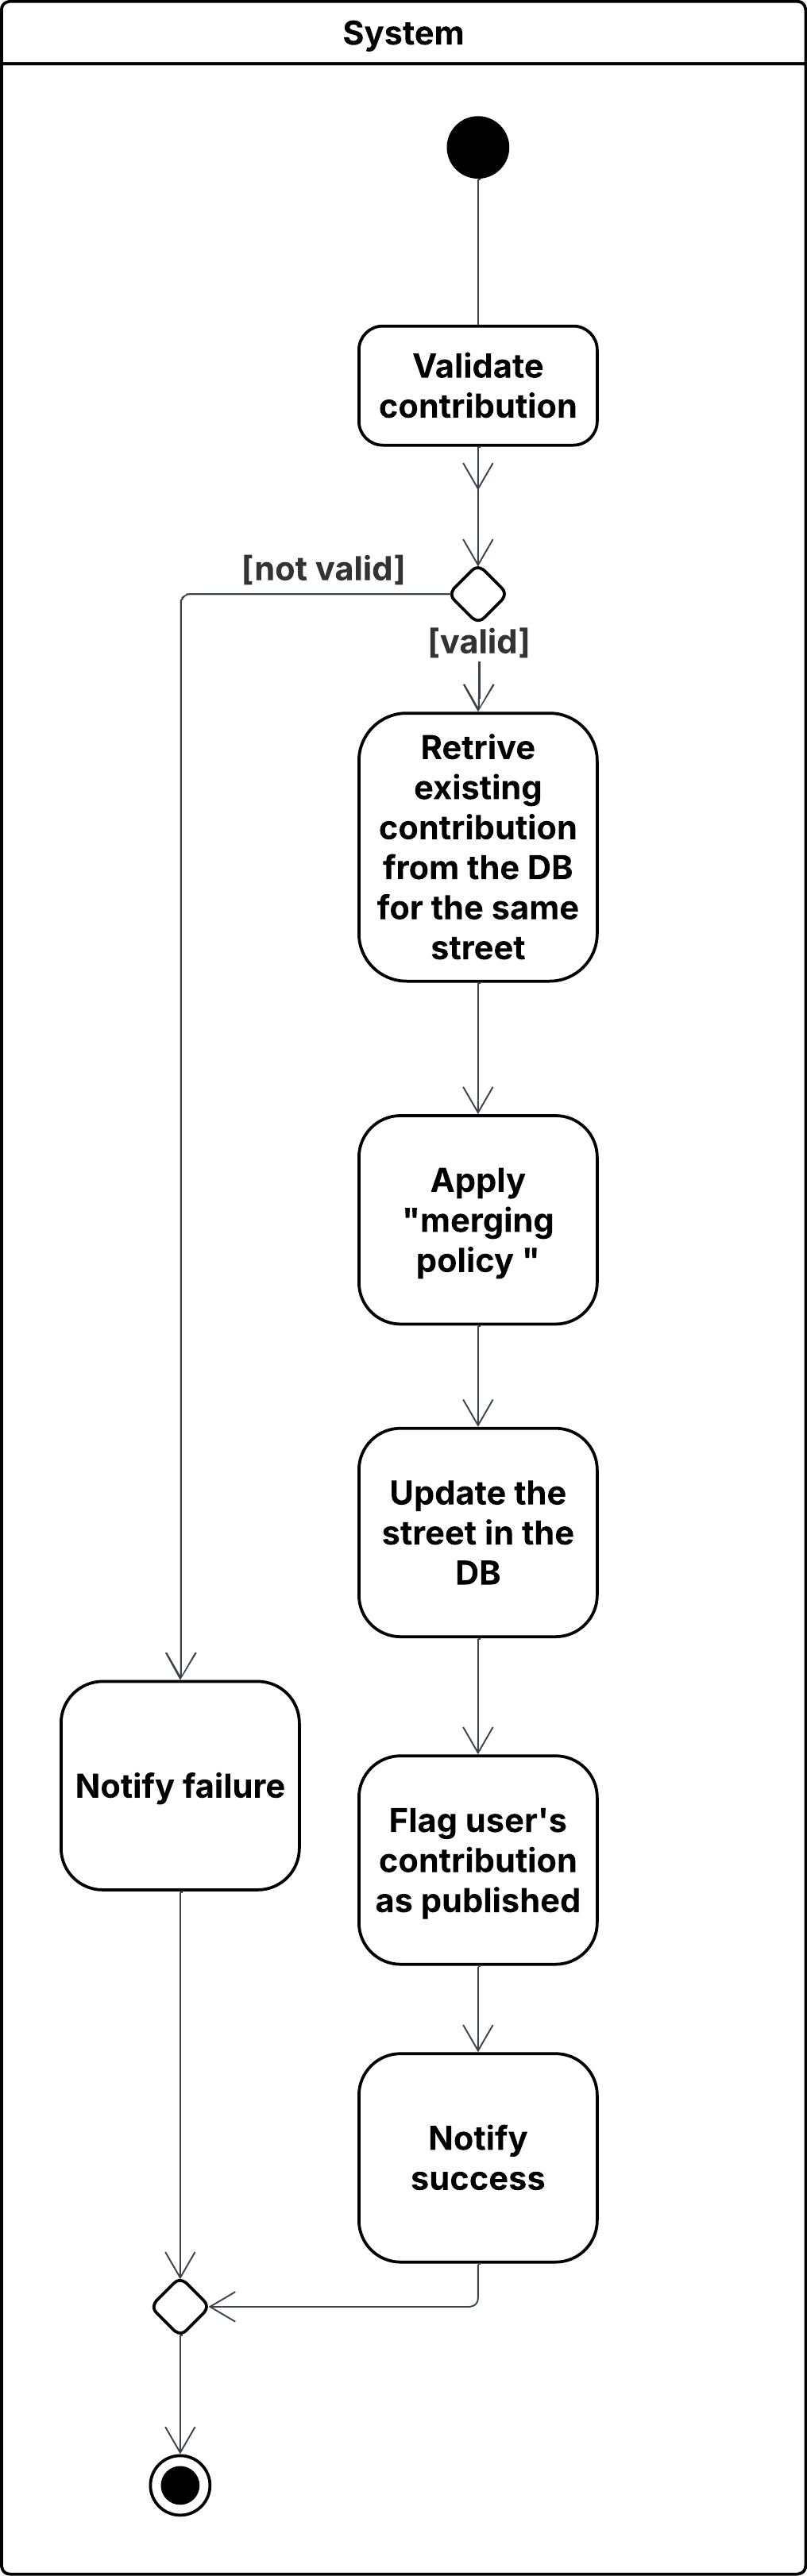
\includegraphics[width=0.4\linewidth]{RASD/Version1.0/images/activity diagram/UC7.png}
         \caption{Publish Contribution}
         \label{fig:publish_contribution}
     \end{center}
\end{figure}

\newpage


\subsubsection*{UC\cuc . View Map}
\begin{center}
    \begin{longtable}{|l|p{0.75\linewidth}|}
        \hline
        \textbf{Actor}            & User \\
        \hline
        \textbf{Entry Conditions} & The User is logged into the platform and has access to the map functionality. \\
        \hline
        \textbf{Flow of Events}    
        & \cucsteps. The User clicks on the ``Map'' section. \\
        & \cucsteps. The system loads the default map region (e.g., around the User's current position or last viewed area). \\
        & \cucsteps. The system retrieves the visible bike-path data for the current map region. \\
        & \cucsteps. The system displays the map together with the visible paths and their associated contributions (e.g., obstacles, warnings, roadworks). \\
        & \cucsteps. The User chooses an action on the map view (e.g., search for a path, tap on a displayed path segment, move around the map, or start following a path). \\
        & \cucsteps. If the User searches for a specific path or destination, the system invokes the \hyperref[search_path]{\uline{UC.~Search Path}} use case and, after the search is completed, updates the map with the best suggested paths (e.g., top 5). \\
        & \cucsteps. If the User taps on a displayed path, the system shows the selected path with more detailed information, including aggregated contributions along that path. \\
        & \cucsteps. If the User decides to follow a selected path, the system redirects the User to the ``Automatic trip mode'' page and invokes the \hyperref[sec:uc_follow_path]{\uline{UC.~Follow Path}} use case. \\
        & \cucsteps. If the User simply moves around the map (pan/zoom), the system retrieves bike-path data for the newly visible region and refreshes the map with updated paths and contributions. \\
        & \cucsteps. For readability, the activity diagram omits that the User can exit the map or return to previous sections of the application at any time during the interaction. \\
        \hline
        \textbf{Exit Conditions}   & The User has visualized the desired map area, inspected the available paths and related contributions, and optionally started following a selected path.\\
        \hline
        \textbf{Exceptions}       & {%
            \begin{itemize}[leftmargin=*]
                \item No bike-path data is available for the current map region: the system still displays the map but shows an informative message indicating that no paths are present.
                \item A temporary error occurs while retrieving path data or contributions: the system notifies the User of the failure and suggests retrying the operation.
            \end{itemize}
        } \\
        \hline
    \end{longtable}
\end{center}



\begin{figure}[H]
    \begin{center}
         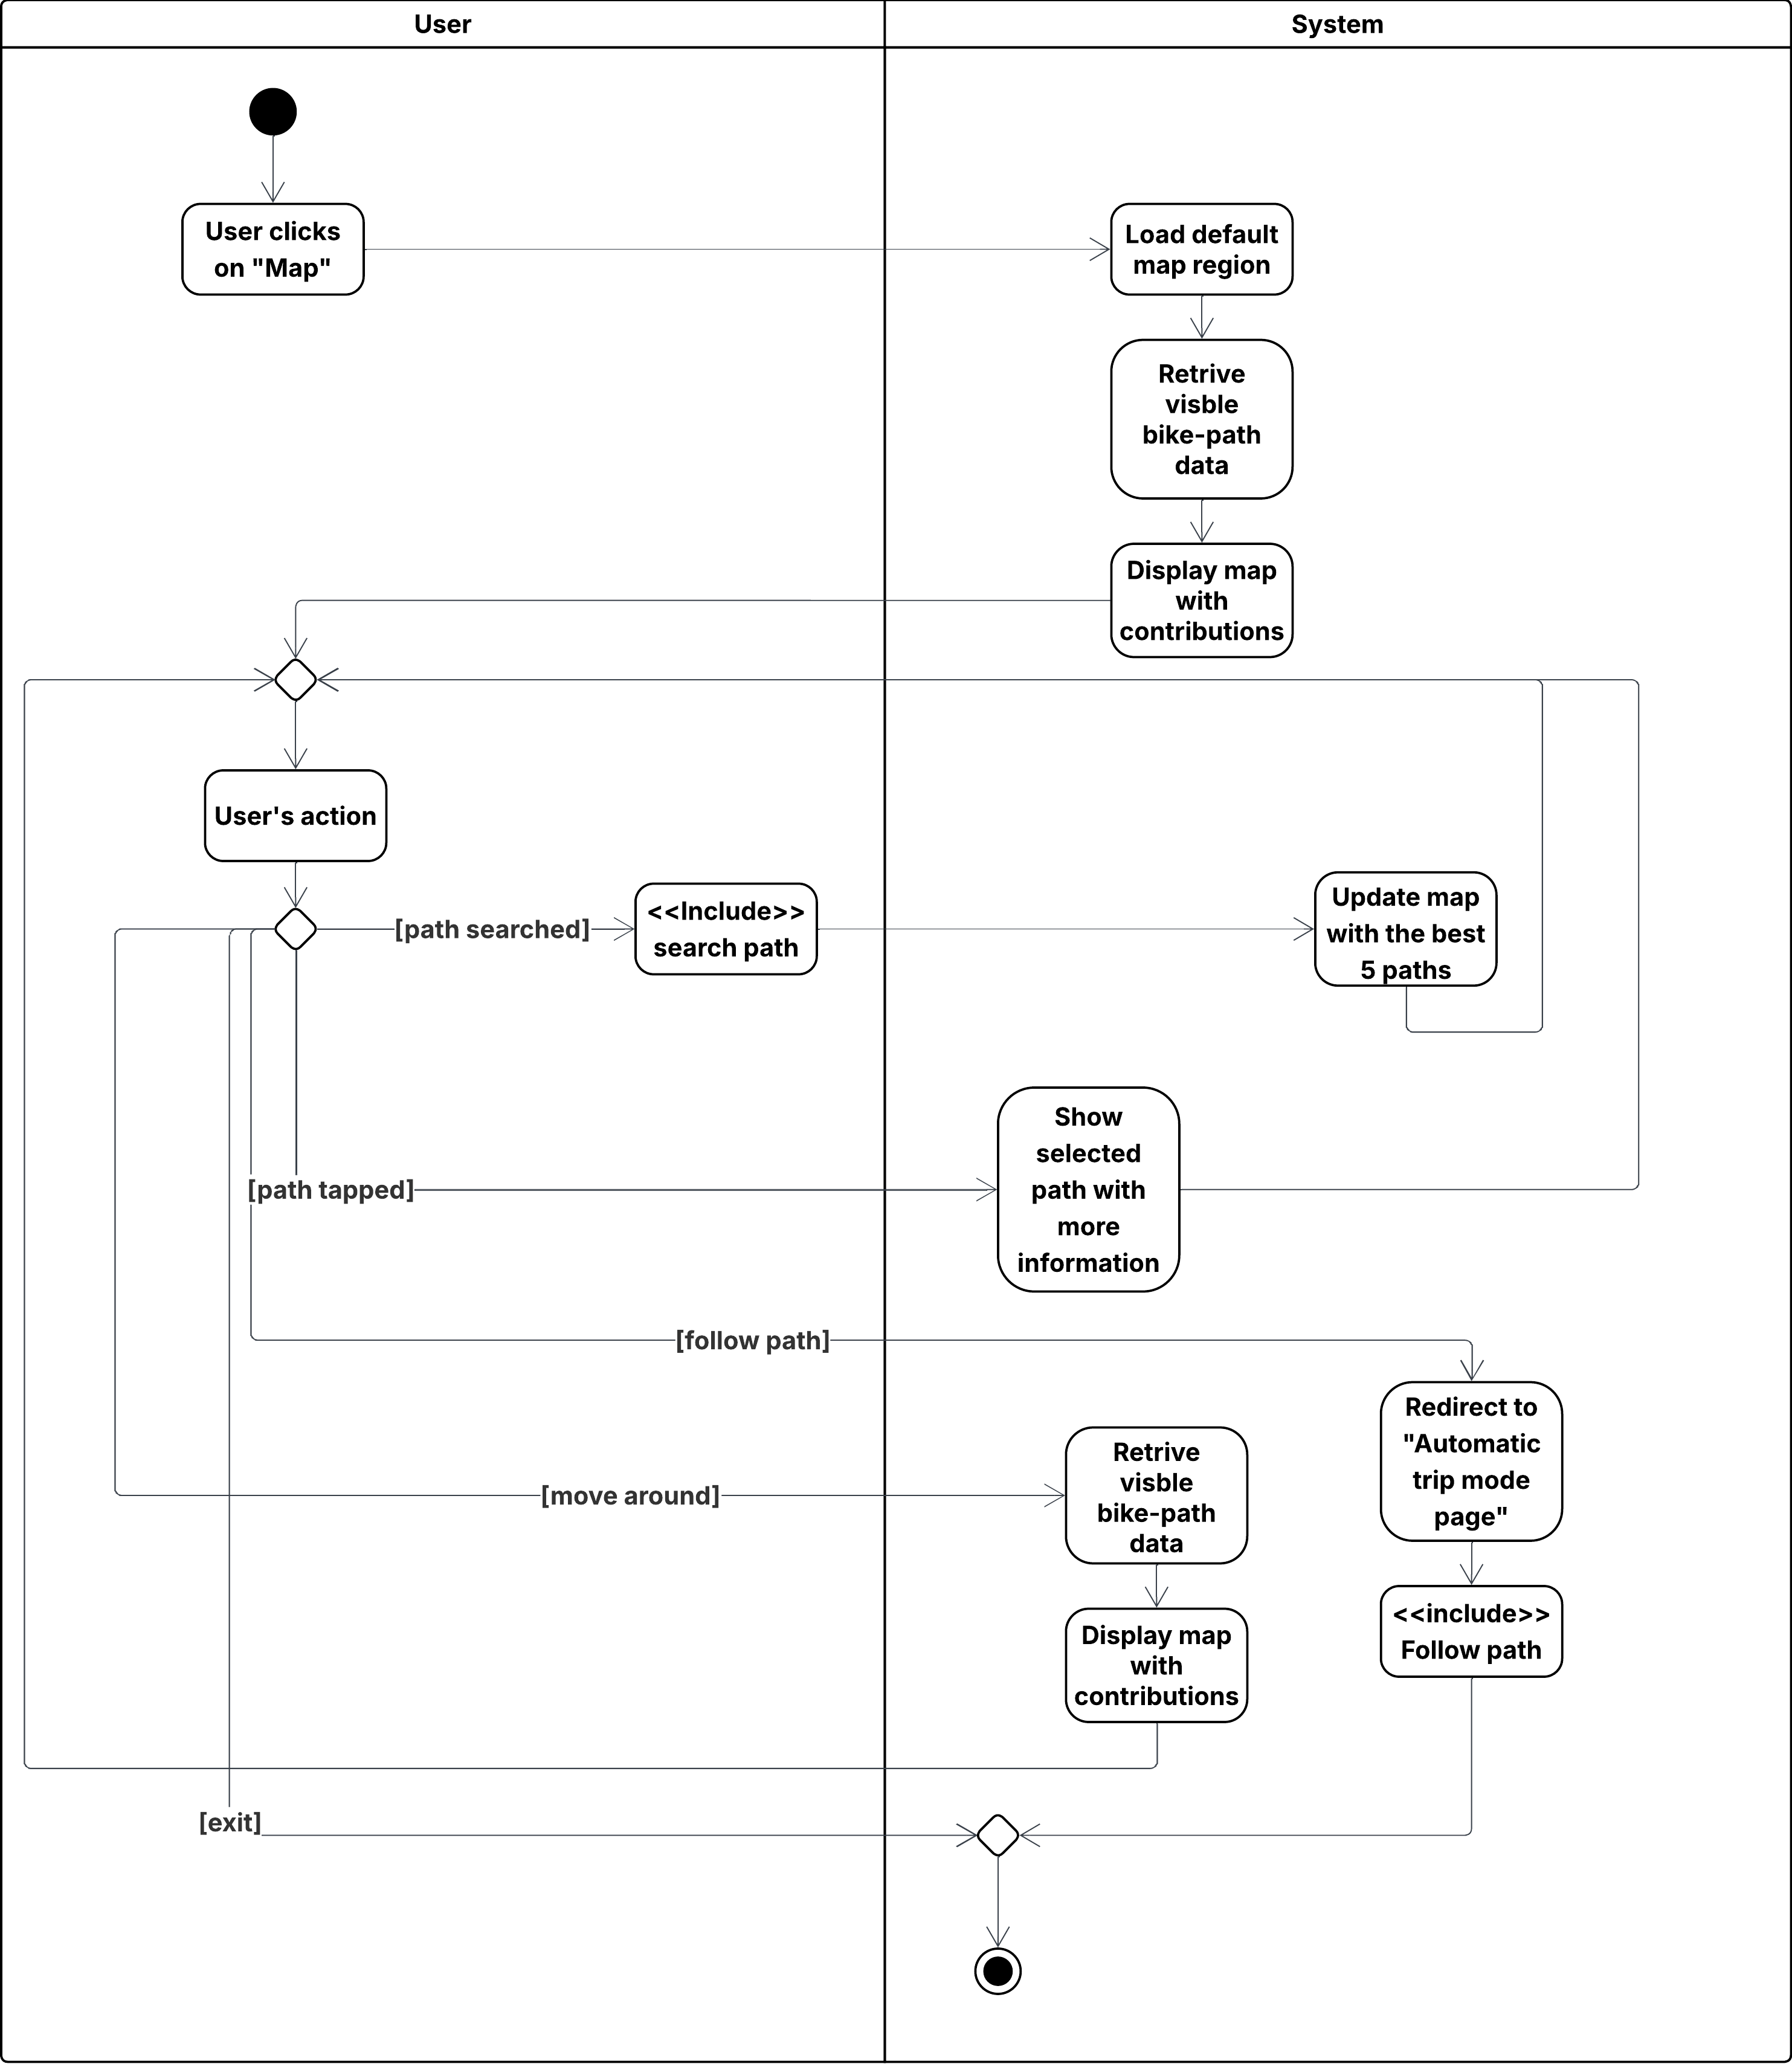
\includegraphics[width=1\linewidth]{RASD/Version1.0/images/activity diagram/UC8.png}
         \caption{View Map}
         \label{fig:view_map}
     \end{center}
\end{figure}

\newpage

\subsubsection*{UC\cuc . Search Path}
\label{sec:uc_search_path}
\begin{center}
    \begin{longtable}{|l|p{0.75\linewidth}|}
        \hline
        \textbf{Actor}            & User \\
        \hline
        \textbf{Entry Conditions} & The User is on a page where the map and the path search functionality are available (e.g., from \hyperref[view_map]{\uline{UC.~View Map}}). \\
        \hline
        \textbf{Flow of Events}    
        & \cucsteps. The User specifies the start and end points of the desired path (e.g., origin and destination on the map or via textual input). \\
        & \cucsteps. The system retrieves from the database the bike paths that connect the specified start and end points, if any exist. \\
        & \cucsteps. The system checks whether the User is registered or unregistered. \\
        & \cucsteps. If the User is registered, the system orders the retrieved paths according to the User's saved preferences and the trips recently completed by the User (e.g., preferred difficulty, usual routes). \\
        & \cucsteps. The system returns the list of searched bike paths to the invoking use case, already ordered if the User is registered. \\
        \hline
        \textbf{Exit Conditions}   & A set of bike paths matching the specified start and end points is produced and made available to the calling functionality.\\
        \hline
        \textbf{Exceptions}       & {%
            \begin{itemize}[leftmargin=*]
                \item No bike path exists connecting the specified start and end points: the system returns an empty result and may provide an informative message to the User.
                \item A temporary error occurs while retrieving paths from the database: the system notifies the failure and suggests the User to retry the search.
            \end{itemize}
        } \\
        \hline
    \end{longtable}
\end{center}




\begin{figure}[H]
    \begin{center}
         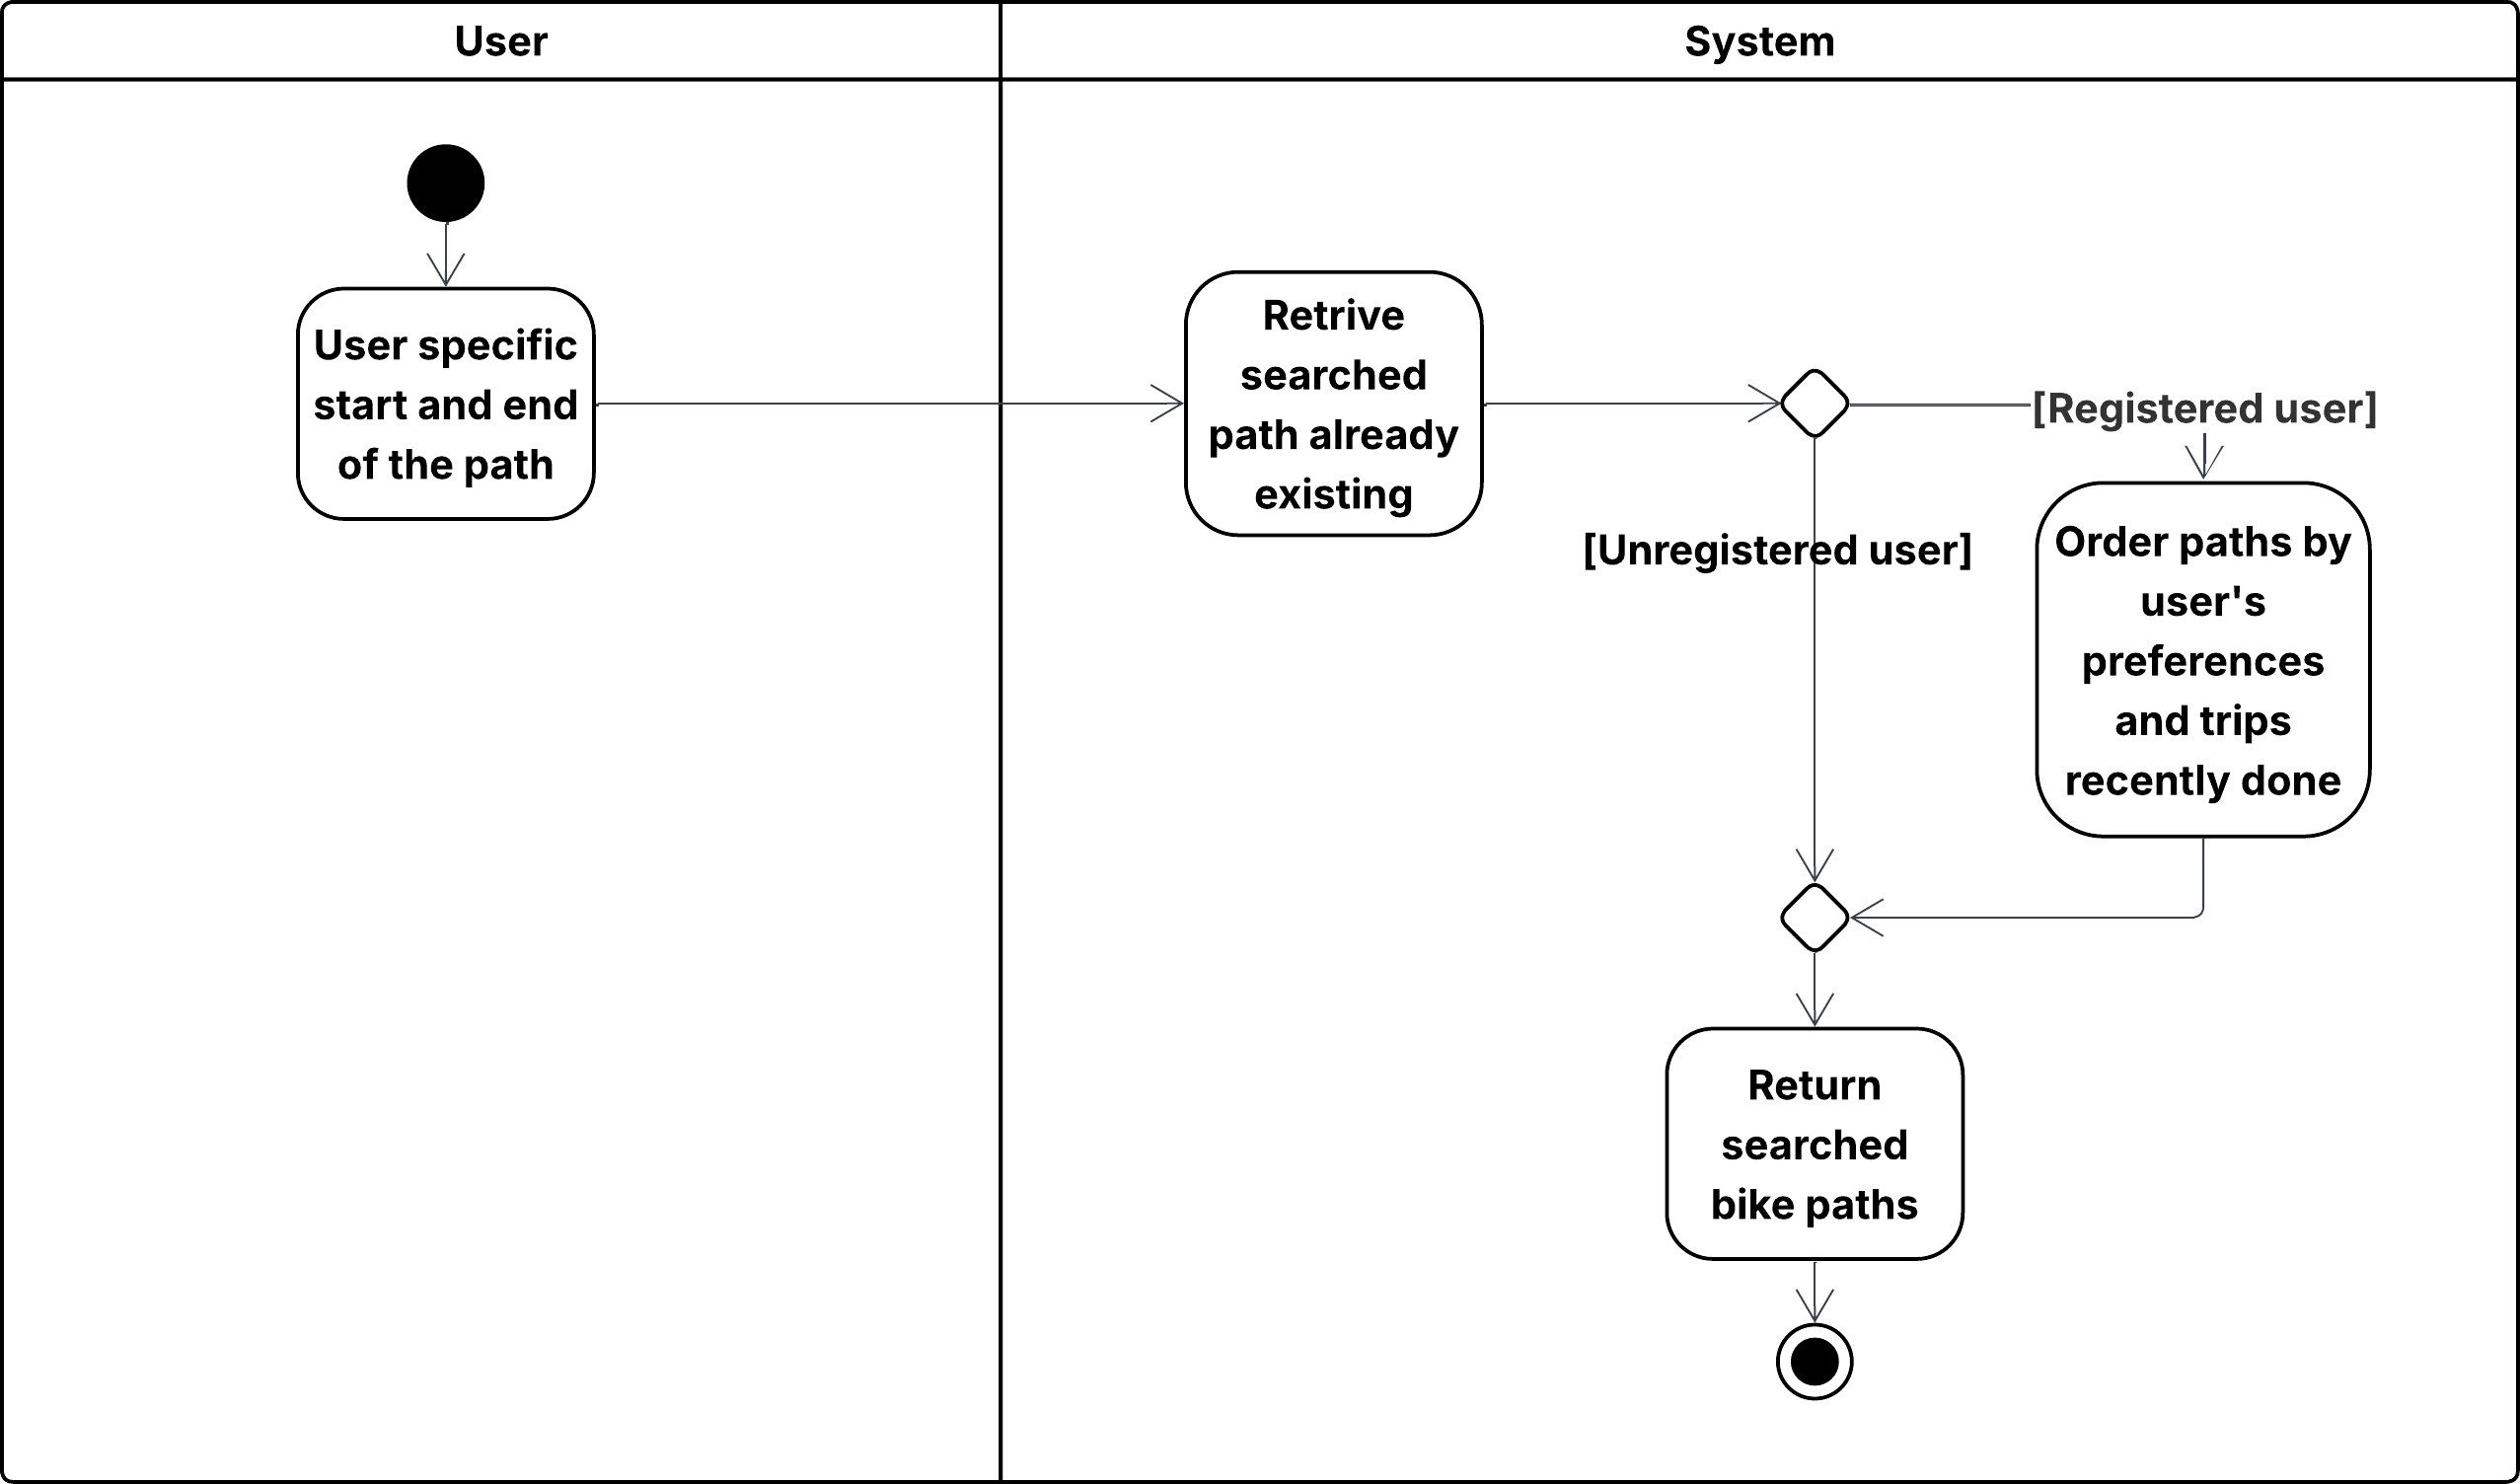
\includegraphics[width=0.8\linewidth]{RASD/Version1.0/images/activity diagram/UC9.png}
         \caption{Search Path}
         \label{fig:search_path}
     \end{center}
\end{figure}

\newpage



\subsubsection*{UC\cuc . Manual Insertion}
\begin{center}
    \begin{longtable}{|l|p{0.75\linewidth}|}
        \hline
        \textbf{Actor}            & Registered User \\
        \hline
        \textbf{Entry Conditions} & The Registered User is logged into the platform and has access to the manual trip insertion functionality. \\
        \hline
        \textbf{Flow of Events}    
        & \cucsteps. The system loads the default map region and initializes an empty \textit{TripDraft}. \\
        & \cucsteps. The User chooses how to add bike paths to the TripDraft (e.g., by manually selecting streets on the map or by searching for existing paths). \\
        & \cucsteps. If the User chooses to search for a path, the system invokes \hyperref[sec:uc_search_path]{\uline{UC.~Search Path}} and lets the User select one of the returned paths. \\
        & \cucsteps. For each selected or manually specified street, the system adds the corresponding bike path to the TripDraft and updates the map accordingly. \\
        & \cucsteps. The system asks the User whether the definition of the trip is finished; the User may repeat the previous step to add more streets. For readability, the activity diagram does not explicitly show that the User can also remove or adjust previously selected streets. \\
        & \cucsteps. Once the trip definition is complete, the system checks the validity of the TripDraft (e.g., at least one street, consistent geometry). If the TripDraft is not valid, the system shows an error and asks the User to correct it. \\
        & \cucsteps. The User chooses an action on the completed TripDraft (e.g., add contributions, save as trip, publish as report, or discard). \\
        & \cucsteps. If the User decides to add contributions, the User selects a street from the TripDraft and specifies a Contribution describing the status of that street (e.g., potholes, obstacles, roadworks). \\
        & \cucsteps. The system checks the validity of each added Contribution and, if a Contribution is not valid, removes it from the TripDraft and notifies the User. \\
        & \cucsteps. If the User chooses to save the TripDraft as a trip, the system saves the trip in the User's history and asks whether the associated Contributions should also be published (following the same iterative publication mechanism described for trips). \\
        & \cucsteps. If the User chooses to publish the information only as a report, the system treats the selected street and its Contribution as a standalone report, publishes the Contribution (without saving the TripDraft as a trip), and updates the corresponding path information. \\
        & \cucsteps. If the User chooses not to publish any Contribution, the system simply saves the trip in the User's history without publishing. \\
        & \cucsteps. If the User decides to discard the TripDraft, the system deletes all temporary data and terminates the use case. \\
        \hline
        \textbf{Exit Conditions}   & The User has either saved a manually defined trip (optionally with published Contributions), published one or more standalone reports about specific streets, or discarded the manual insertion.\\
        \hline
        \textbf{Exceptions}       & {%
            \begin{itemize}[leftmargin=*]
                \item The TripDraft is not valid (e.g., no street selected or inconsistent data): the system notifies the error and does not allow the User to save or publish until the trip is corrected.
                \item One or more Contributions added to the TripDraft are not valid (e.g., missing mandatory fields): the system removes the invalid Contributions and asks the User to review them.
                \item A temporary error occurs while saving the trip or publishing Contributions: the system notifies the failure and suggests the User to retry the operation.
            \end{itemize}
        } \\
        \hline
    \end{longtable}
\end{center}


\begin{figure}[H]
    \begin{center}
         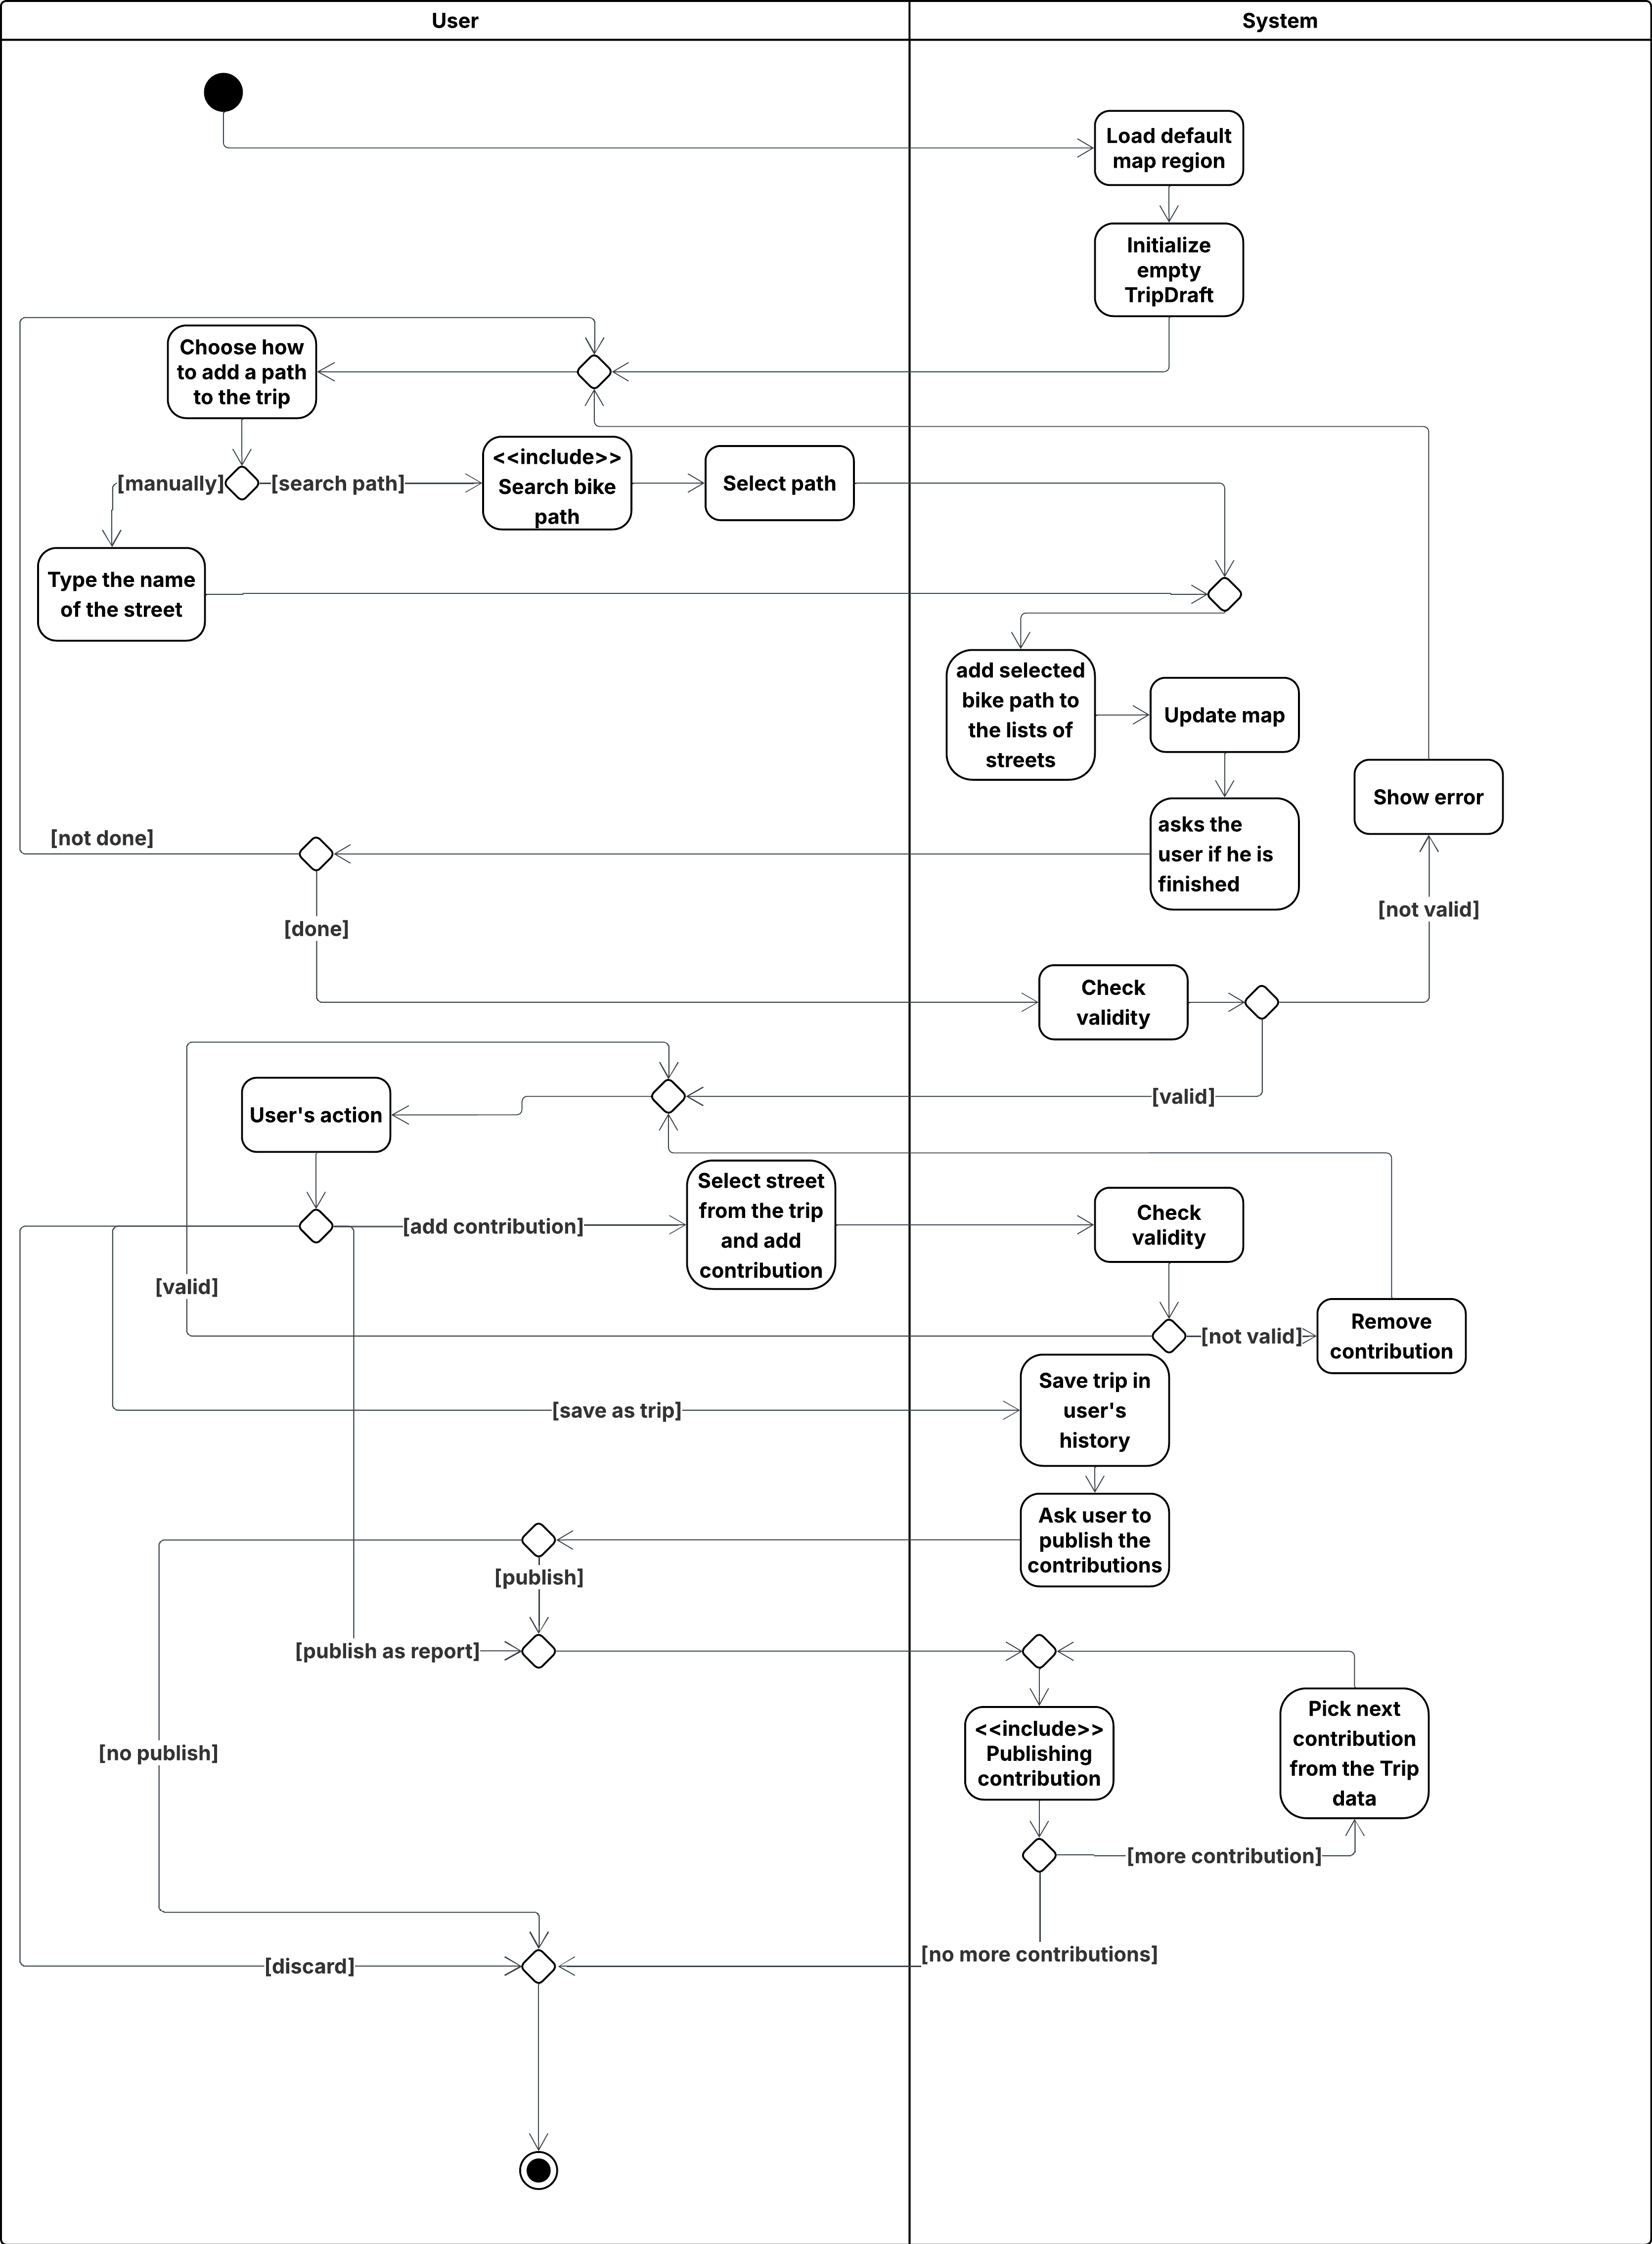
\includegraphics[width=1\linewidth]{RASD/Version1.0/images/activity diagram/UC10.png}
         \caption{Manual Insertion}
         \label{fig:manual_insertion}
     \end{center}
\end{figure}

\newpage

\subsubsection*{UC\cuc . Automatic Insertion}
\label{sec:uc_automatic_insertion}
\begin{center}
    \begin{longtable}{|l|p{0.75\linewidth}|}
        \hline
        \textbf{Actor}            
        & Registered User \\
        \hline
        \textbf{Entry Conditions} 
        & The Registered User is logged into the platform and has a device with GPS and motion sensors enabled. \\
        \hline
        \textbf{Flow of Events}    
        & \cucsteps. The User presses the ``Start recording'' button to begin an automatic trip. \\
        & \cucsteps. The system initializes a new \textit{RecordingSession} on the Client device. \\
        & \cucsteps. The system starts GPS tracking and activates accelerometer and gyroscope monitoring. \\
        & \cucsteps. While the recording is active, the system periodically acquires GPS samples and motion sensor data, storing them locally as raw trip data. \\
        & \cucsteps. In parallel, the system monitors the User’s movement to detect interruptions: consecutive GPS positions are compared and, if the distance travelled remains below a configurable threshold for a given time window, the User is marked as stationary; when movement resumes, the stationary status is cleared. \\
        & \cucsteps. The recording continues until the system receives an ``End recording'' event from the User. \\
        & \cucsteps. When the recording is stopped, the system stops GPS and motion sensors and finalizes the collection of raw trip data. \\
        & \cucsteps. The system reconstructs the full path of the trip from the collected GPS trace. \\
        & \cucsteps. Immediately after the recording phase, the system performs an inference process on the collected sensor data in order to generate a set of \textit{draft Contributions} associated with the reconstructed path. These Contributions are not published nor merged at this stage and are intended solely for User review. \\
        & \cucsteps. The system invokes the Data Enrichment Service, which computes aggregated trip statistics (e.g., distance, duration, speed profiles) and enriches the trip with external contextual information, such as weather data associated with the GPS trace, as described in \hyperref[sec:uc_enrich_trip_weather]{\uline{UC.~Enrich Trip with Weather Information}}. \\
        & \cucsteps. The system redirects the User to the ``Review and edit'' screen and includes \hyperref[sec:uc_edit_trip]{\uline{UC.~Edit Trip}}, allowing the User to inspect the automatically generated trip, modify its path if necessary, and edit, remove, or add Contributions before making any decision about saving or publishing the trip. \\
        \hline
        \textbf{Exit Conditions}   
        & An automatic trip has been recorded with its reconstructed path, a set of draft Contributions generated through post-processing inference, and enriched contextual and statistical information; control is transferred to the manual review and editing phase. \\
        \hline
        \textbf{Exceptions}       
        & {%
            \begin{itemize}[leftmargin=*]
                \item GPS or motion sensors are not available or cannot be started: the system notifies the User and does not start the automatic recording.
                \item A temporary error occurs while acquiring sensor data: the system attempts to continue recording with partial data and informs the User that some portions of the trip may be incomplete.
            \end{itemize}
        } \\
        \hline
    \end{longtable}
\end{center}






\begin{figure}[H]
    \begin{center}
         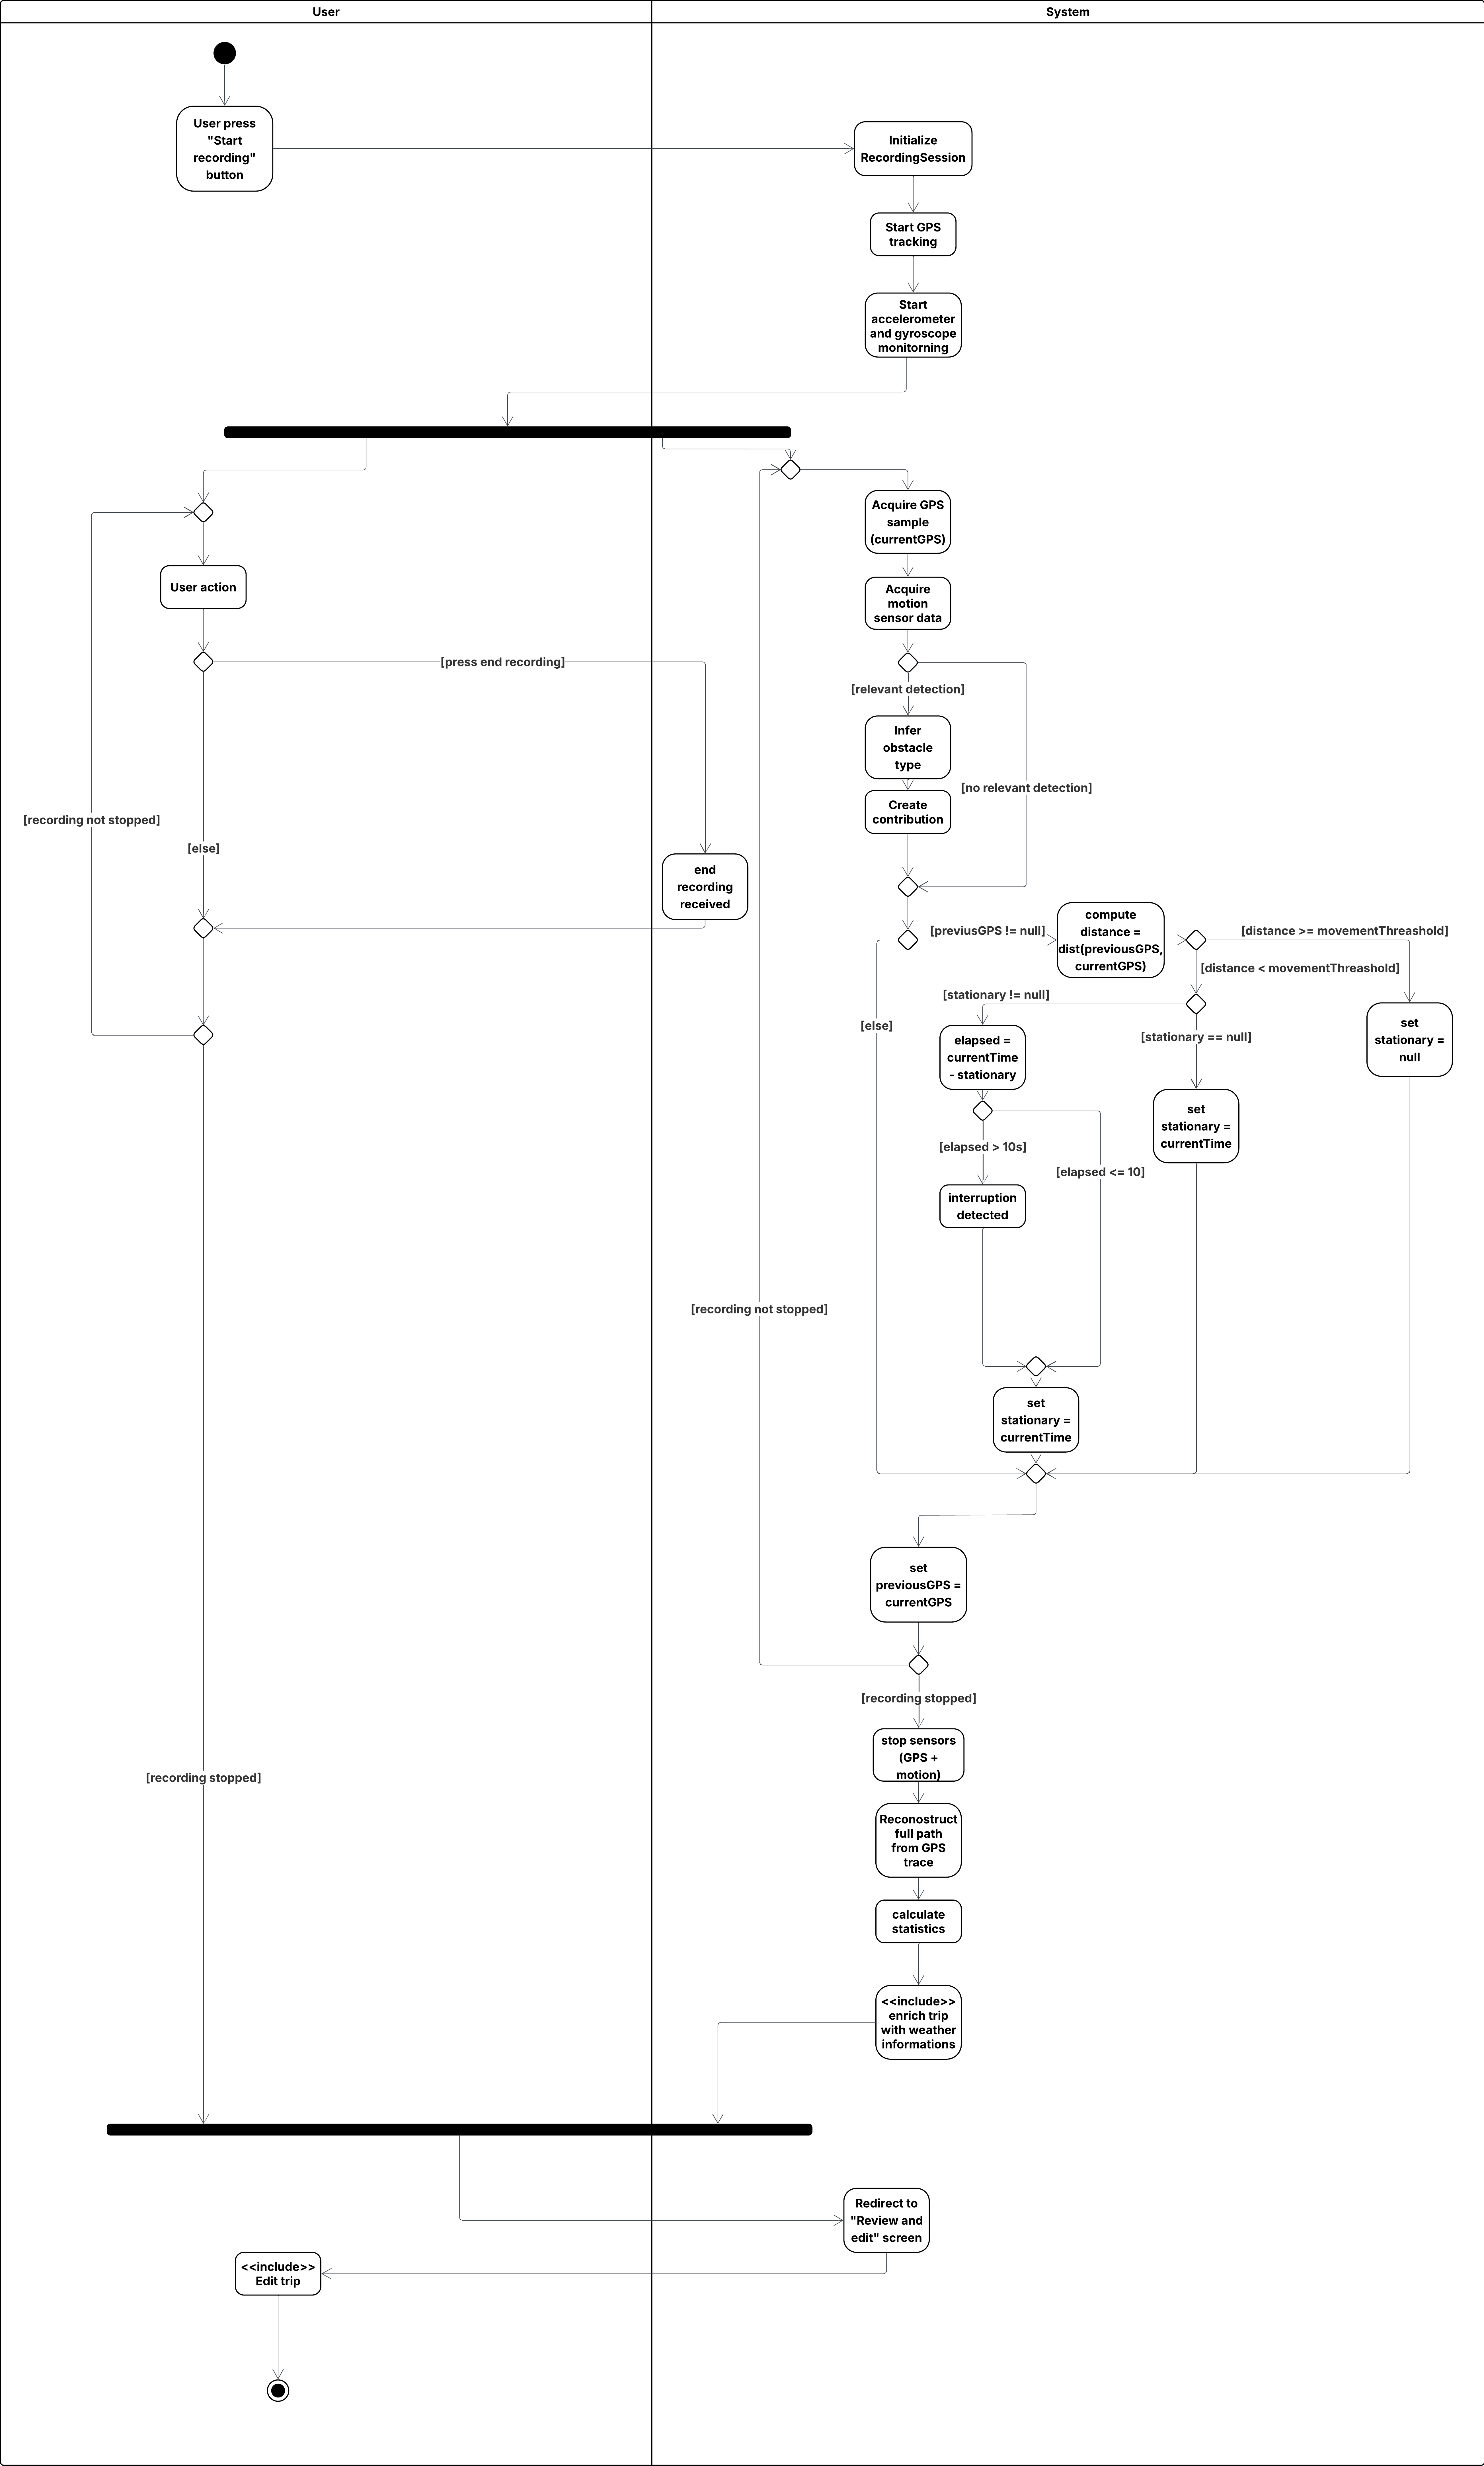
\includegraphics[width=0.85\linewidth]{RASD/Version1.0/images/activity diagram/UC11.png}
         \caption{Automatic Insertion}
         \label{fig:automatic_insertion}
     \end{center}
\end{figure}

\newpage

\subsubsection*{UC\cuc . Enrich Trip with Weather Information}
\label{sec:uc_enrich_trip_weather}
\begin{center}
    \begin{longtable}{|l|p{0.75\linewidth}|}
        \hline
        \textbf{Actor}            & System (Weather Service as external actor) \\
        \hline
        \textbf{Entry Conditions} & A TripDraft has been created and its GPS trace with timestamps is available. \\
        \hline
        \textbf{Flow of Events}    
        & \cucsteps. The system prepares a weather request using the trip's GPS trace and associated timestamps (e.g., start/end time and representative points along the route). \\
        & \cucsteps. The system sends the request to the external Weather Service API. \\
        & \cucsteps. The Weather Service receives the weather request. \\
        & \cucsteps. The Weather Service checks its availability for the given time and location. \\
        & \cucsteps. If the service is available, the Weather Service fetches the weather conditions corresponding to the requested time/place and returns the weather data to the system. \\
        & \cucsteps. If the service is not available or an internal error occurs, the Weather Service returns an error response to the system instead of weather data. \\
        & \cucsteps. Upon receiving the response, the system checks whether the request completed without errors. \\
        & \cucsteps. If no error occurred, the system attaches the retrieved weather data to the TripDraft so that it can be stored together with the trip and shown in the trip details. \\
        & \cucsteps. If an error occurred, the system marks the trip as ``no weather data available'' and continues without weather enrichment. \\
        \hline
        \textbf{Exit Conditions}   & The TripDraft is enriched with weather information associated with its GPS trace, or it is explicitly marked as having no weather data available.\\
        \hline
        \textbf{Exceptions}       & {%
            \begin{itemize}[leftmargin=*]
                \item The Weather Service is temporarily unavailable or returns an error: the system marks the trip as ``no weather data available'' and does not retry immediately.
                \item The GPS trace is incomplete or does not contain valid timestamps: the system does not send the request to the Weather Service and leaves the TripDraft without weather information.
            \end{itemize}
        } \\
        \hline
    \end{longtable}
\end{center}


\begin{figure}[H]
    \begin{center}
         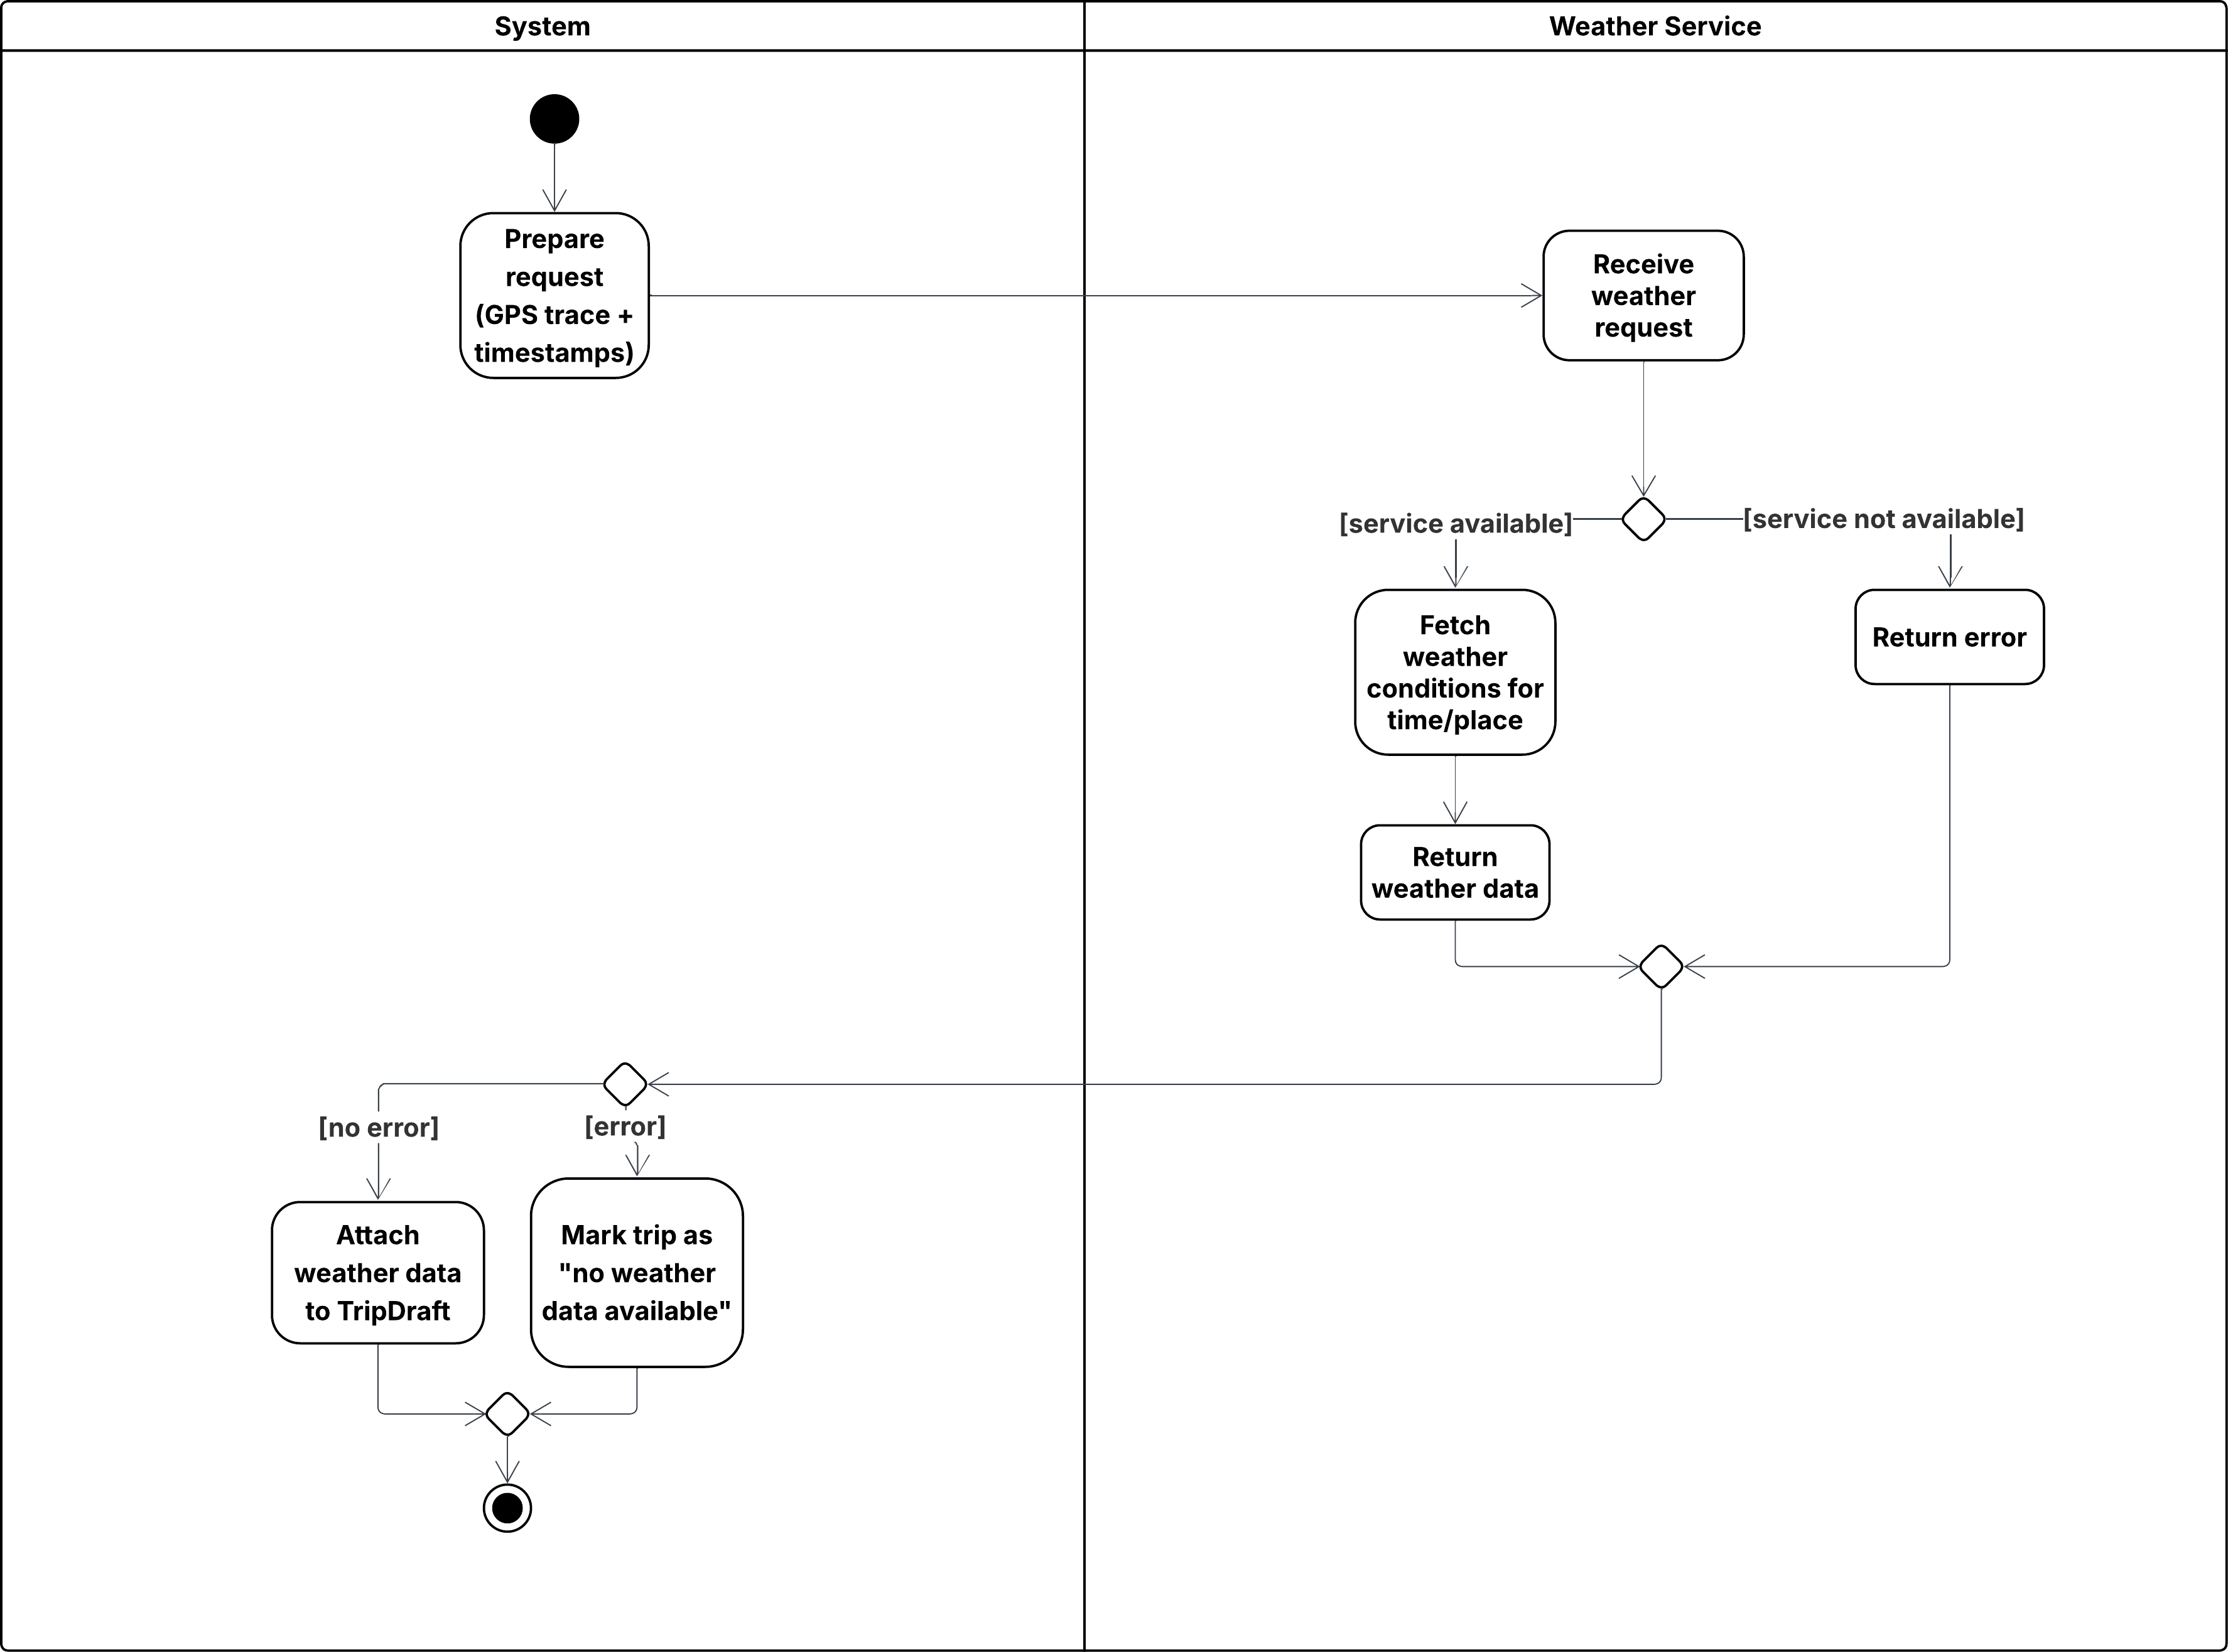
\includegraphics[width=1\linewidth]{RASD/Version1.0/images/activity diagram/UC12.png}
         \caption{Enrich Trip with Weather Information}
         \label{fig:uc_enrich_trip_with_weather_information}
     \end{center}
\end{figure}

\newpage



\subsubsection*{UC\cuc . Edit Trip}
\label{sec:uc_edit_trip}
\begin{center}
    \begin{longtable}{|l|p{0.75\linewidth}|}
        \hline
        \textbf{Actor}            & Registered User \\
        \hline
        \textbf{Entry Conditions} & A recorded trip (automatic defined) and its associated draft Contributions are available for review (at the end of recording). \\
        \hline
        \textbf{Flow of Events}    
        & \cucsteps. The system shows the trip together with the obstacles and Contributions that have been automatically detected. \\
        & \cucsteps. The User inspects the detected obstacles and Contributions and may confirm them, adjust their details, or remove the ones considered incorrect. \\
        & \cucsteps. The User can also add missing Contributions for streets included in the trip by selecting a street and specifying additional information (e.g., a new obstacle or warning). \\
        & \cucsteps. After reviewing the Contributions, the User chooses an action (e.g., store only, store and publish, or discard). \\
        & \cucsteps. If the User chooses to \textit{store and publish}, the system iteratively processes the Contributions associated with the trip: for each Contribution, the system invokes \hyperref[sec:uc_publish_contribution]{\uline{UC.~Publish Contribution}} and then selects the next Contribution until there are no more. \\
        & \cucsteps. Once all Contributions have been processed, the system stores the trip in the User's history together with the final set of Contributions. \\
        & \cucsteps. If the User chooses to \textit{store} without publishing, the system skips the publication step and only stores the trip and its Contributions in the User's history as private data. \\
        & \cucsteps. If the User decides to \textit{discard}, the system deletes the trip data and all associated draft Contributions, terminating the use case. \\
        \hline
        \textbf{Exit Conditions}   & The trip is either stored (with or without published Contributions) in the User's history, or it has been completely discarded.\\
        \hline
        \textbf{Exceptions}       & {%
            \begin{itemize}[leftmargin=*]
                \item An error occurs while storing the trip or its Contributions: the system notifies the User of the failure and suggests retrying the operation; no partial or inconsistent trip data is left saved.
                \item An error occurs during the publication of a Contribution (in the included UC Publish Contribution): the system notifies the User and leaves the affected Contribution in a non-published state while still allowing the rest of the trip to be stored.
            \end{itemize}
        } \\
        \hline
    \end{longtable}
\end{center}


\begin{figure}[H]
    \begin{center}
         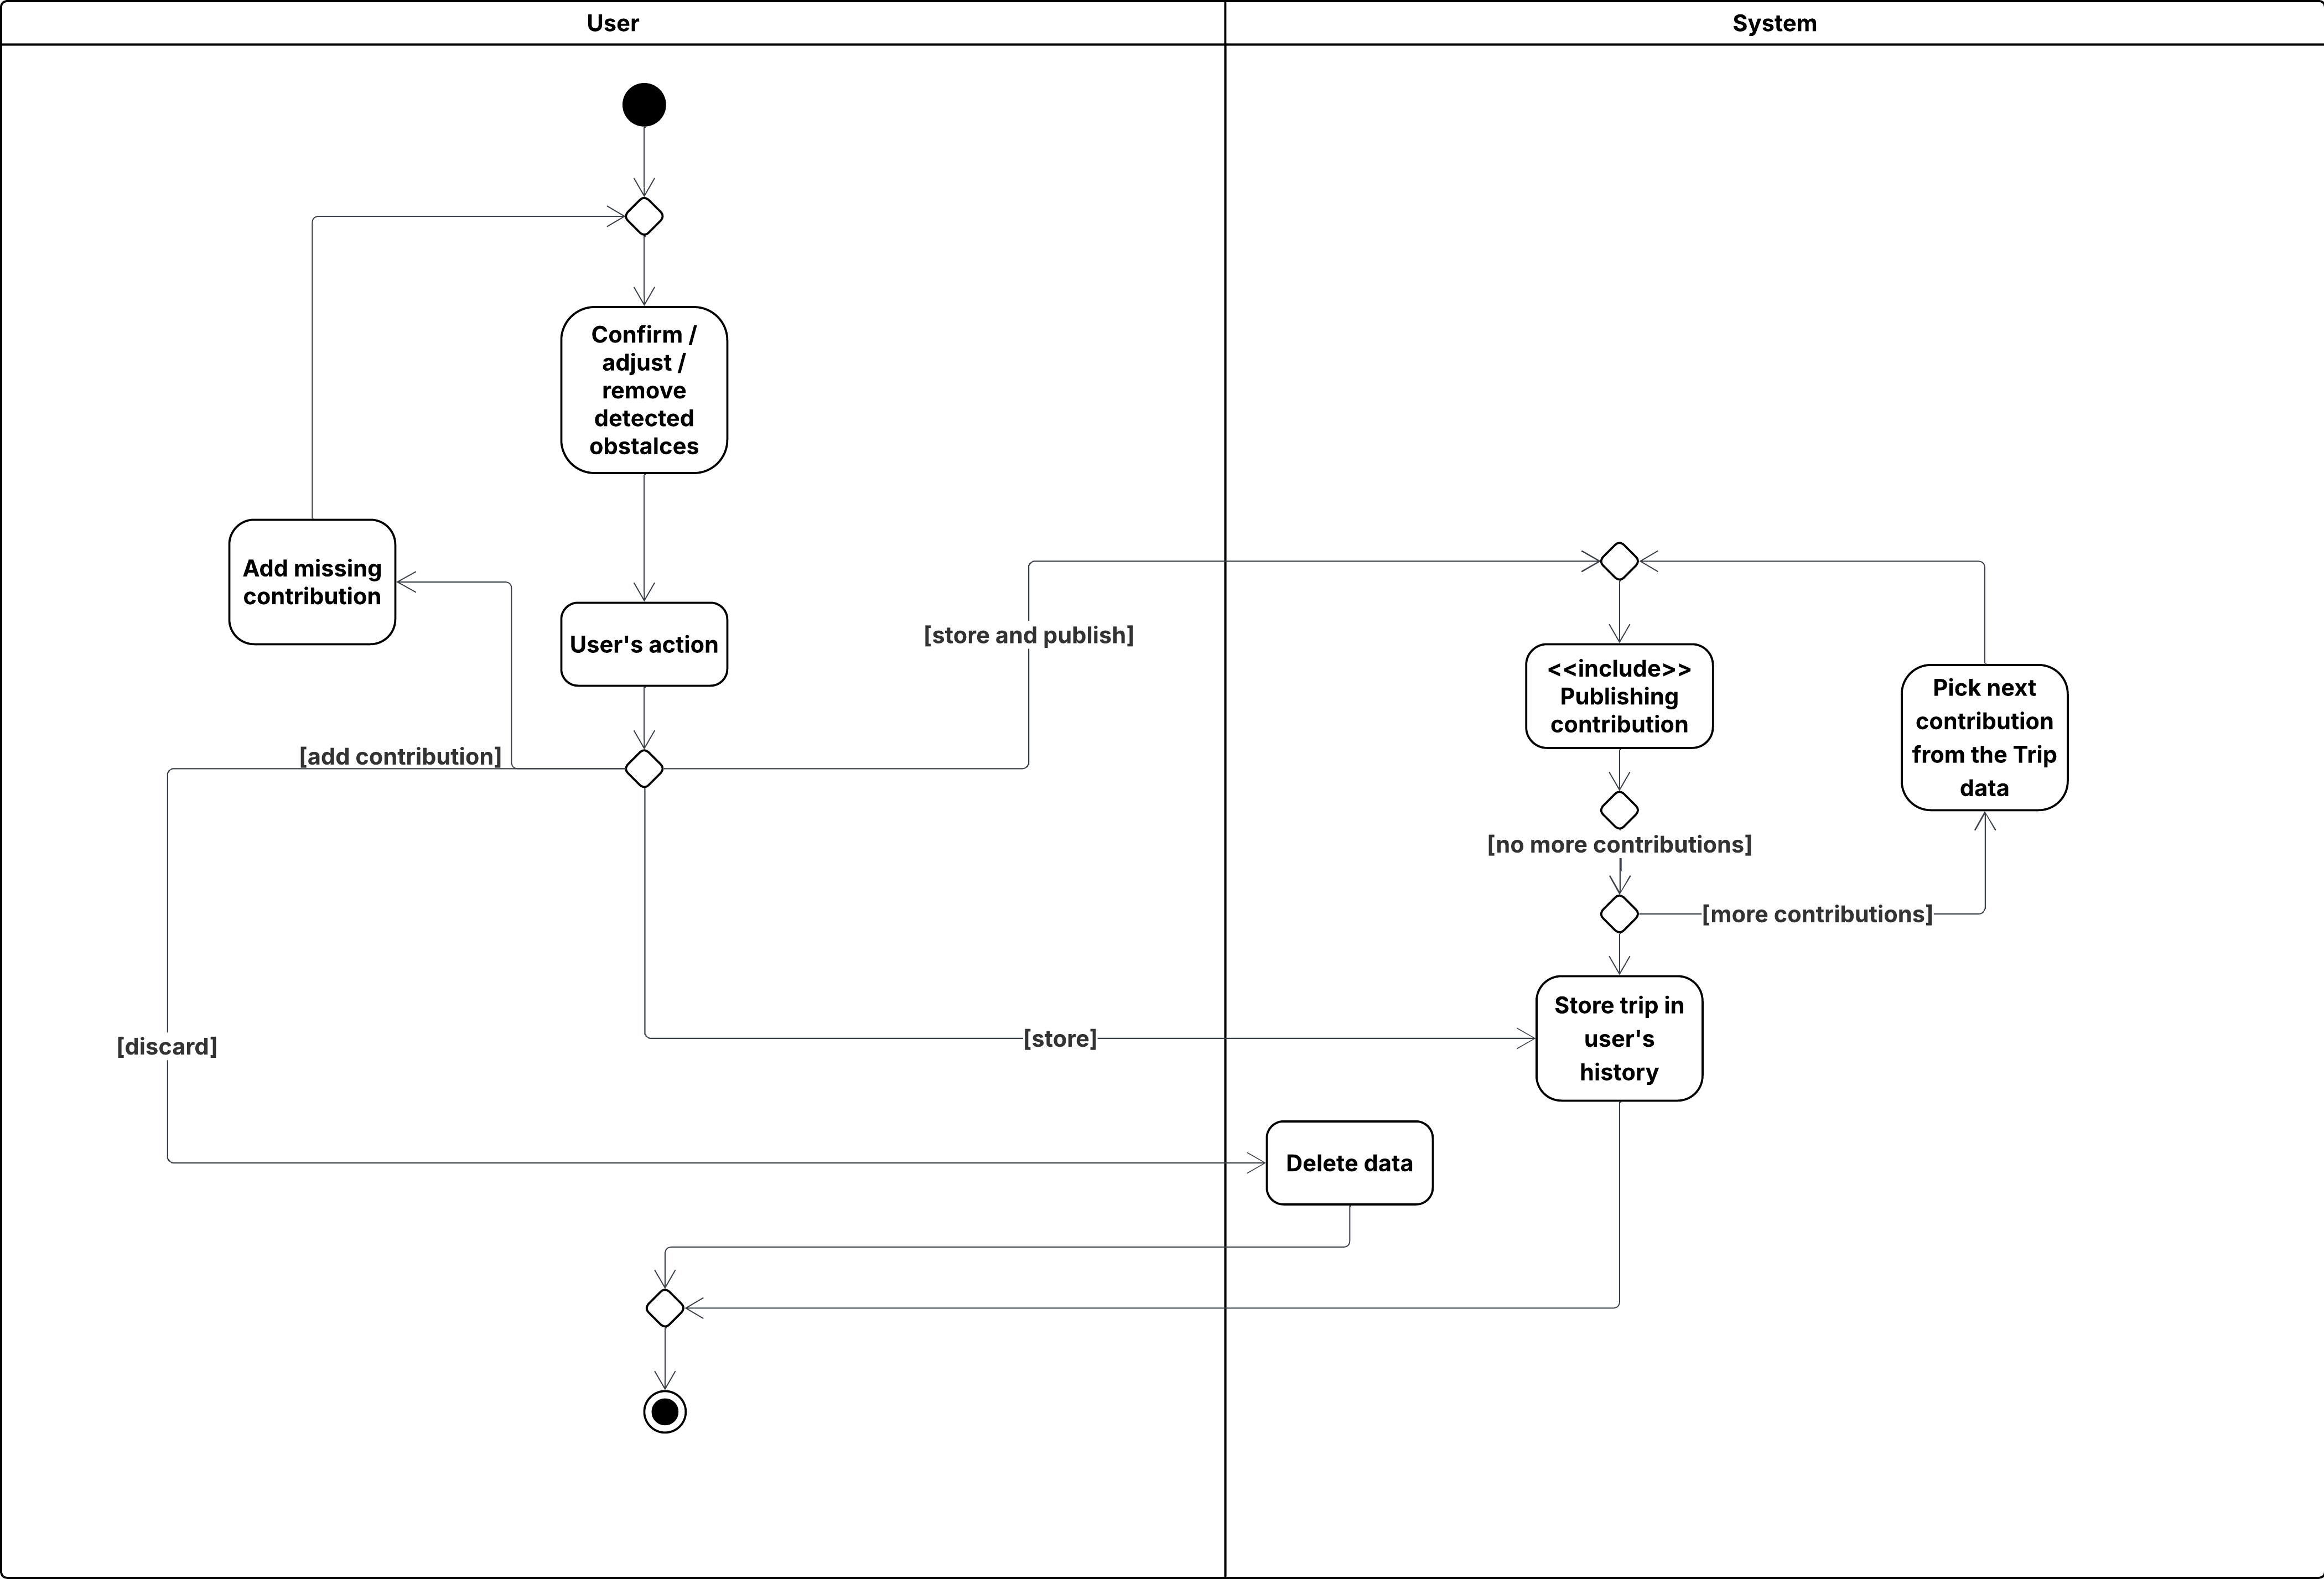
\includegraphics[width=0.9\linewidth]{RASD/Version1.0/images/activity diagram/UC13.png}
         \caption{Edit Trip}
         \label{fig:uc_edit_trip}
     \end{center}
\end{figure}

\newpage



\subsubsection*{UC\cuc . Follow Path (extends UC.~Automatic Insertion)}
\begin{center}
    \begin{longtable}{|l|p{0.75\linewidth}|}
        \hline
        \textbf{Actor}            & Registered User \\
        \hline
        \textbf{Entry Conditions} & 
        The User has selected a path from the map (see \hyperref[sec:uc_view_map]{\uline{UC.~View Map}}) and chooses to follow it. \\
        \hline
        \textbf{Flow of Events}    
        & \cucsteps. The system highlights the selected path on the map and opens a dedicated ``Follow path'' view. \\
        & \cucsteps. The User starts recording, triggering \hyperref[sec:uc_automatic_insertion]{\uline{UC.~Automatic Insertion}} for the current session. \\
        & \cucsteps. While the recording is active, the map keeps the chosen path visually highlighted; the User is free to follow it or deviate from it, and the system does not recompute or enforce the route. \\
        & \cucsteps. All other behaviours (trip recording, obstacle inference, interruption detection, reconstruction of the path, statistics computation and subsequent review/edit) follow exactly the flow described in UC.~Automatic Insertion. \\
        \hline
        \textbf{Exit Conditions}   & 
        An automatic trip has been recorded while a selected path was highlighted on the map; the resulting trip is then handled as in UC.~Automatic Insertion (review, edit, store, publish). \\
        \hline
        \textbf{Exceptions}       & {%
            \begin{itemize}[leftmargin=*]
                \item Sensors or GPS are not available: the system notifies the User and does not start the follow-path recording.
            \end{itemize}
        } \\
        \hline
    \end{longtable}
\end{center}
\noindent\textit{Remark.}
Since the behaviour of this use case is almost identical to \hyperref[sec:uc_automatic_insertion]{\uline{UC.~Automatic Insertion}},
apart from the highlighted path on the map and the absence of route recalculation, no dedicated activity diagram is provided.



\subsection{Mapping On Requirements}
\label{subsec:mapping_on_requirements}

\newcounter{row}
\setcounter{row}{1}
\newcommand{\crow} {\therow\stepcounter{row}}

\begin{longtable}{
    |>{\centering\arraybackslash}p{2cm}
    |>{\centering\arraybackslash}p{2.5cm}
    |>{\centering\arraybackslash}p{5cm}
    |>{\centering\arraybackslash}p{3.5cm}
    |>{\centering\arraybackslash}p{2.5cm}|
}
    \hline
    \textbf{Row ID} & \textbf{Goal ID} & \textbf{Req ID} & \textbf{DA ID} & \textbf{UC ID} \\ \hline
    \endfirsthead
    \hline
    \textbf{Row ID} & \textbf{Goal ID} & \textbf{Req ID} & \textbf{DA ID} & \textbf{UC ID} \\ \hline
    \endhead
    \hline
    \endfoot
    \hline
    \endlastfoot

    \crow & G1 & R1, R2, R3, R4 & DA3, DA4, DA5 & UC1, UC2, UC3, UC4, UC5 \\ \hline
    \crow & G2 & R2, from R5 to R13, R34, R35 & DA1, DA2, DA3, DA6, DA7, DA8, DA9, DA12, & from UC10 to UC14 \\ \hline
    \crow & G3 & R7, R8, R10, R14, R34, R35 & DA1, DA2, DA6, DA7, DA9, DA10, DA11 & UC6, UC13 \\ \hline
    \crow & G4 & R2, R10, R11, R12, R13 & DA3, DA12, DA13 & UC10, UC13 \\ \hline
    \crow & G5 & R2, R5, R6, R7, R8, R9, R10, R11, R34, R35 & DA3, DA6, DA7, DA9 DA10, DA11, & UC11, UC12, UC14 \\ \hline
    \crow & G6 & R2, from R15 to R20 & DA3 &  UC7 \\ \hline
    \crow & G7 & from R24 to R33 & DA1, DA2, DA3, DA11 & UC8, UC9 \\ \hline
    \crow & G8 & R19, R20, R21, R22, R23, R24 & DA1, DA2, DA14 & UC7\\ %\hline
    
    %\crow & G9 & R19, R21, R33, R34 & DA1, DA8, DA9, DA10, DA15, DA16 & UC7, UC10, UC11, UC14 \\ \hline
    %\crow & G10 & R20, R21, R23, R24--R30, R33, R34 & DA1, DA2, DA8, DA9, DA10, DA12, DA15, DA16 & UC7, UC8, UC9, UC10, UC11, UC14 

\label{tab:traceability}
\end{longtable}




\section{Performance Requirements}

The system gives real time information to its users, so it is critical that it provides a smooth and responsive user experience on mobile devices under normal operating conditions therefore:

\begin{itemize}
    \item The system shall provide a \textbf{responsive user interface}, ensuring that standard user interactions (e.g., navigation between screens, map panning and zooming, profile access) are completed within \textbf{0.5 seconds} under normal network conditions.
    
    \item Map rendering and updates, including the visualization of bike paths and aggregated contributions, shall be completed within \textbf{2 seconds} after the user changes the visible map area or performs a path search.
    
    \item The system shall support \textbf{real-time trip recording}, continuously collecting GPS and sensor data without causing noticeable delays, application freezes, or data loss during normal usage.
    
    \item Sensor data acquisition (e.g., GPS, accelerometer, gyroscope) shall not exceed acceptable latency thresholds that could compromise the accuracy of recorded trips or obstacle detection.
    
    \item The system shall be capable of handling \textbf{concurrent access by 15000 users} without degradation of core functionalities, such as map visualization, path search, and trip recording.
    
    \item Data synchronization between the mobile application and the backend server shall occur within a reasonable time frame, ensuring that newly recorded trips and contributions are available to the user within \textbf{30 seconds} after successful upload.
    
    \item The system shall ensure acceptable performance under varying network conditions, gracefully handling temporary connectivity issues by caching essential data locally and synchronizing it once the connection is restored.
\end{itemize}

\section{Design Constraints}

\subsubsection{3.4.1 Standards Compliance}
\begin{itemize}
    \item The system shall be developed in accordance with the guidelines and best practices for native mobile applications provided by \textbf{Android} and \textbf{iOS} platforms, including the official Android Developer Guidelines and Apple Human Interface Guidelines.
    
    \item The system shall comply with the \textbf{ISO/IEC/IEEE 29148:2018} standard for requirements engineering, ensuring consistency and traceability between requirements and design decisions.
    
    \item All data exchanged between the mobile application and backend services shall use secure communication protocols compliant with \textbf{HTTPS} and \textbf{TLS} standards.
    
    \item The system shall follow recognized \textbf{mobile security best practices}, including secure credential handling, encrypted local storage where required, and protection against common vulnerabilities such as unauthorized data access.
    
    \item The system shall adhere to applicable \textbf{data protection and privacy regulations}, including the \textbf{GDPR}, ensuring transparency in the collection, storage, and processing of personal and location-based data.
    
    \item The system shall comply with standard accessibility guidelines for mobile applications, such as the \textbf{WCAG 2.1} principles where applicable, to ensure usability for users with different abilities.
\end{itemize}

\subsubsection{3.4.2 Hardware Limitations}
\begin{itemize}
    \item The system shall operate within the hardware constraints typical of mobile devices, including limited CPU resources, memory, storage capacity, and battery life.
    
    \item The application shall be optimized to function correctly on devices with heterogeneous hardware configurations, ensuring acceptable performance on both high-end and mid-range smartphones.
    
    \item Continuous use of hardware components such as \textbf{GPS}, \textbf{accelerometer}, and \textbf{gyroscope} shall be managed efficiently to minimize battery consumption and prevent excessive resource usage.
    
    \item The system shall handle cases in which required hardware components are unavailable, disabled or denied by the user by providing appropriate feedback and gracefully degrading affected functionalities.
\end{itemize}


\section{Software System Attributes}

\subsubsection{3.5.1 Reliability}
\begin{itemize}
    \item The system shall ensure correct and consistent behavior during normal operation, minimizing unexpected crashes or data loss.
    
    \item The system shall preserve recorded trip data and user contributions in the presence of temporary failures, such as application restarts or network interruptions.
    
    \item The system shall detect and handle runtime errors, providing informative feedback to the user when an operation cannot be completed.
\end{itemize}

\subsubsection{3.5.2 Availability}
\begin{itemize}
    \item The system shall be available for use whenever the mobile device is operational and has network connectivity.
    
    \item Core functionalities such as trip recording and data visualization shall remain usable even during temporary backend unavailability, relying on local storage and deferred synchronization.
    
    \item The system shall support background execution, where permitted by the operating system, to ensure continuity of trip recording.
\end{itemize}

\subsubsection{3.5.3 Security}
\begin{itemize}
    \item The system shall protect user data by enforcing authentication mechanisms and secure session management.
    
    \item Sensitive information, including credentials and personal data, shall be transmitted exclusively through encrypted channels using HTTPS and TLS.
    
    \item The system shall restrict access to user-specific data, ensuring that each user can only view and modify their own information.
    
    \item The system shall request explicit user consent before accessing sensitive hardware components, such as GPS and motion sensors.
\end{itemize}

\subsubsection{3.5.4 Maintainability}
\begin{itemize}
    \item The system shall be designed following modular and layered architectural principles to facilitate maintenance and future enhancements.
    
    \item The codebase shall be documented and structured to support debugging, testing, and incremental updates.
    
    \item The system shall allow updates and bug fixes to be deployed without requiring changes to user data or system reconfiguration.
\end{itemize}

\subsubsection{3.5.5 Portability}
\begin{itemize}
    \item The system shall be portable across the supported mobile platforms, namely Android and iOS.
    
    \item Platform-specific components shall be isolated to minimize the effort required to adapt the application to different operating system versions.
    
    \item The system shall support future migration to additional mobile platforms with limited changes to the core application logic.
\end{itemize}






   \chapter{Formal Analysis using Alloy}
\label{ch:formal_analysis_using_alloy}

\section{Objectives}
The formal modeling activity has been carried out using Alloy 6 with the purpose of validating and ensuring the correctness of the core processes of the Best Bike Paths (BBP) system. The primary objectives of this modeling activity are the following:

\subsection{Consistent System Evolution}
We have modeled the rules that define the system's dynamic evolution over time. For each action, we have specified the preconditions that must hold for its execution and the postconditions that describe its effects. Frame conditions have been used to guarantee that elements not involved in an action remain unchanged. In particular, we focused on the following critical actions:
\begin{itemize}
    \item Saving a trip by a registered user
    \item Publishing a contribution
    \item Linking a contribution to a trip
    \item Confirming a detection
    \item Merging contributions
\end{itemize}
By defining these actions carefully, we ensured that the system’s evolution remains consistent and predictable under all possible sequences of interactions.

\subsection{Contribution and Detection Management Logic}
We have formalized how contributions and detections are managed in the system, including their creation, association with trips, publication, and eventual merging. The model guarantees that each contribution is linked to exactly one trip and one author, and that detection confirmations correctly generate contributions without introducing inconsistencies.

These parts of the system are the most critical, as they capture the complex interactions between registered users, trips, and the dynamic data collected from the environment. To keep the model tractable and understandable, we intentionally omitted less critical aspects, such as user deletion or detailed weather data processing, focusing on the key functionalities needed to validate system behavior. 

\textbf{Note:} The merging logic has been simplified for the sake of clarity; specifically, the automatic transformation of \texttt{BikeSuitability} information was decoupled from the primary \texttt{merge} predicate due to its complexity. However, the impact of these suitability updates on the environment was still rigorously verified within the final functional scenario (\texttt{PathBreakScenario}).



\section{The Model}

\subsection{Modular Structure}
The Alloy model of BBP has been organized modularly by separating \textbf{signatures}, \textbf{predicates}, \textbf{facts}, and \textbf{main scenarios} into different files:

\begin{itemize}
    \item \textbf{Signatures (signatures.als)} define the structural elements of the system, including users, trips, contributions, detections, street segments, paths, and supporting entities such as weather information. Enum types like \texttt{Score} capture qualitative attributes of streets and contributions.
    \item \textbf{Predicates (predicates.als)} describe the core actions of the system. Each predicate specifies the preconditions for executing the action, the postconditions describing the resulting state, and the frame conditions that ensure elements not affected by the action remain unchanged.
    \item \textbf{Facts (facts.als)} enforce the consistency of the world. They guarantee, for instance, that each contribution belongs to exactly one trip, authorship is consistent, paths are topologically connected, and scores are correctly propagated. Facts ensure that the system evolves only according to the defined actions, preventing spontaneous or invalid state changes.
    \item \textbf{Main module (main.als)} defines the initial state of the system and models its evolution over time. It also contains test scenarios to validate typical interactions, such as saving a trip, publishing contributions, confirming detections, and merging contributions. The \texttt{doNothing} predicate ensures idle transitions preserve consistency, while the \texttt{System} predicate allows all valid evolutions according to the defined actions.
\end{itemize}

This modular organization allows for clear reasoning about each aspect of the system and facilitates automatic analysis using Alloy. The model provides a foundation to verify that BBP behaves as intended under different sequences of user interactions and environmental inputs.

\subsection{Signatures}

This file contains the definitions of the Signatures of the main entities in the Best Bike Paths (BBP) system. 
BBP supports users in recording and browsing bike paths, either manually or automatically. The main entities 
modeled are Users (Registered and Unregistered), Trips (Manual and Automatic), Detections, Contributions, 
Paths, Street Segments, and auxiliary types such as WeatherInfo and Score. Fields have been defined using 
\texttt{one} or \texttt{set} cardinalities to avoid unnecessary complexity and improve model performance. 
Constraints for each Signature are defined to ensure that instances are always meaningful and consistent. 

\noindent\rule{\linewidth}{0.4pt} % linea di divisione

\begin{lstlisting}[language=alloy, caption={Alloy Signatures}, label={lst:signatures}]
module signatures

open util/boolean

// --- BASIC ENTITIES ---

sig Coordinate {}

one sig WeatherService {}

sig WeatherInfo {}

// --- USERS ---

var abstract sig User {}

var sig UnregisteredUser extends User {}

var sig RegisteredUser extends User {
    // Dynamic relations tracking a user's activity
    var contributions: set Contribution,
    var trips: set Trip
}

// --- TRIPS ---

var abstract sig Trip {
    var contributions: set Contribution,
    var madeOf: set StreetSegment
}

var sig ManualTrip extends Trip {}

var sig AutomaticTrip extends Trip {
    // Automatic trips include external weather data and sensor detections
    var weatherData: lone WeatherInfo,
    var detections: set Detection
}

// --- DETECTIONS ---

var sig Detection {
    var detectedInfo: one Information,
    var onStreet: one StreetSegment,
    var confirmed: one Bool,
    var score: one Score
} 

// --- INFORMATION ---

var abstract sig Information {
    var position: one Coordinate
}

var sig Warning extends Information {}
var sig Event extends Information {}

var abstract sig BikeSuitability extends Information {
    var isSuitable: one Bool
}

var sig SpeedLimUpdate extends BikeSuitability {}
var sig BikeLaneUpdate extends BikeSuitability {}
var sig HeavyTraffic extends BikeSuitability {}

// --- CONTRIBUTIONS ---

var sig Contribution {
    var author: lone RegisteredUser,
    var segment: one StreetSegment,
    var info: set Information,
    var score: one Score
}

// Subset of contributions that have been verified and integrated into the map
var sig PublishedContribution in Contribution {}

// --- PATH GENERATION ---

one sig PathGenerate {
    var activePaths: set Path
}

sig Path {
    // Every path must consist of at least one segment
    segments: some StreetSegment,
    score: one Score
}

// --- STREET SEGMENTS ---

sig StreetSegment {
    start: one Coordinate,
    end: one Coordinate,
    // Attributes that change based on user feedback and processing
    var score: one Score,
    var isCyclable: one Bool
}

// --- ENUMERATIONS ---

enum Score { Optimal, Medium, Sufficient, RequiresMaintenance, None }
\end{lstlisting}

\subsection{Predicates}

This file contains the modeling of the main operations that users can perform in the Best Bike Paths (BBP) system, expressed as Alloy predicates. Each predicate defines preconditions that must hold for the operation to execute, and postconditions that specify the changes in the system state visible in the next instant. Frame conditions are also included to ensure that unrelated parts of the system remain unchanged.

Predicates cover the main functionalities of BBP for managing trips, contributions, and detections, including:
\begin{itemize}
    \item \textbf{saveTrip}: Records a new trip for a registered user.
    \item \textbf{publishContribution}: Publishes a contribution so that it becomes visible to all users.
    \item \textbf{saveContribution}: Links a contribution to a trip and its author.
    \item \textbf{confirmDetection}: Confirms an automatically detected information and converts it into a contribution.
    \item \textbf{merge}: Updates the score of a street segment based on a contribution.
\end{itemize}

\noindent\rule{\linewidth}{0.4pt} % linea di divisione

\begin{lstlisting}[language=alloy, caption={Alloy Predicates for BBP}, label={lst:predicates}]
module predicates

open signatures

// --- SAVE TRIP ---

pred saveTrip[u: RegisteredUser, t: Trip] {
    // Preconditions
    u in RegisteredUser
    all u1: RegisteredUser | t not in u1.trips

    // Postconditions
    u.trips' = u.trips + t
    u.contributions' = u.contributions + t.contributions

    all u2: RegisteredUser - u | u2.trips' = u2.trips

    // Frame conditions
    (Trip <: madeOf)' = (Trip <: madeOf)
    (Trip <: contributions)' = (Trip <: contributions)
    (Trip <: detections)' = (Trip <: detections)

    User' = User
    Contribution' = Contribution
    PathGenerate.activePaths' = PathGenerate.activePaths
    (StreetSegment <: score)' = (StreetSegment <: score)
}

// --- PUBLISH CONTRIBUTION ---

pred publishContribution[u: RegisteredUser, c: Contribution] {
    // Preconditions
    u in RegisteredUser
    c not in PublishedContribution
    c.author = u

    // Postconditions
    PublishedContribution' = PublishedContribution + c

    // User and Author updates
    (RegisteredUser <: contributions)' = (RegisteredUser <: contributions) + (u -> c)
    (c.author)' = u
    some c.(Contribution <: score)'

    // Frame conditions
    User' = User
    Trip' = Trip
    Information' = Information

    trips' = trips
    madeOf' = madeOf
    activePaths' = activePaths
    weatherData' = weatherData
    (StreetSegment <: score)' = (StreetSegment <: score)
}

// --- SAVE CONTRIBUTION (LINKING) ---

pred saveContribution[u: RegisteredUser, t: Trip, c: Contribution] {
    // Preconditions: the contribution must not be already linked
    all u1: RegisteredUser | c not in u1.contributions
    all t1: Trip | c not in t1.contributions

    // Postconditions: establish the link between contribution, author, and trip
    c.author' = u
    t.contributions' = t.contributions + c

    // Frame conditions
    User' = User
    Contribution' = Contribution
    PathGenerate.activePaths' = PathGenerate.activePaths
    trips' = trips
}

// --- CONFIRM DETECTION ---

pred confirmDetection[u: RegisteredUser, t: AutomaticTrip, d: Detection, c: Contribution] {
    // Preconditions: detection must be unconfirmed and belong to the user's trip
    all u1: RegisteredUser | c not in u1.contributions
    all t1: Trip | c not in t1.contributions
    d in t.detections
    d.confirmed = False
    t in u.trips

    // Postconditions: confirm the detection and save it as a contribution
    d.confirmed' = True

    c.segment = d.onStreet
    c.info = d.detectedInfo
    c.score = d.score

    saveContribution[u, t, c]

    // Frame conditions
    User' = User
}

// --- MERGE CONTRIBUTION ---

pred merge[c: Contribution] {
    // Preconditions: only published contributions are merged into the global map
    c in PublishedContribution

    // Postconditions: update the segment's score based on the contribution data
    (c.segment.score)' = c.score

    // Frame conditions
    User' = User
    Trip' = Trip
    Contribution' = Contribution
    madeOf' = madeOf
    activePaths' = activePaths
    PublishedContribution' = PublishedContribution
}
\end{lstlisting}

\subsection{Facts}

This file contains facts for enforcing the consistency of the Best Bike Paths (BBP) system. Facts ensure that the evolution of the system occurs only through the execution of the actions defined in the predicates, and not spontaneously. They impose constraints on the relationships among trips, contributions, detections, street segments, paths, and users, maintaining the internal consistency of the system over time.

\noindent\rule{\linewidth}{0.4pt} % linea di divisione

\begin{lstlisting}[language=alloy, caption={Alloy Facts for BBP}, label={lst:facts}]
module facts

open signatures
open predicates

// --- STRUCTURAL CONSISTENCY ---

fact StructuralConsistency {
    // Each Trip belongs to at most one RegisteredUser
    all t: Trip | lone u: RegisteredUser | t in u.trips

    // Each Contribution belongs to at most one Trip
    all c: Contribution | lone t: Trip | c in t.contributions
}

// --- DETECTIONS & INFORMATION CONSISTENCY ---

fact detectionConsistency {
    // Detections associated with a trip persist in the next state
    all t: Trip, d: Detection |
        d in t.detections implies d in (t.detections)'
}

fact detectedInfoConsistency {
    // Information linked to a detection persists in the next state
    all i: Information, d: Detection |
        i in d.detectedInfo implies i in (d.detectedInfo)'
}

fact streetConsistency {
    // The street segment associated with a detection remains the same over time
    always all s: StreetSegment, d: Detection |
        s in d.onStreet implies s in (d.onStreet)'
}

fact detectionTripConsistency {
    // A single detection cannot belong to two different automatic trips
    always all disj t1, t2: AutomaticTrip | no t1.detections & t2.detections
}

// --- AUTHOR CONSISTENCY ---

fact authorConsistency {
    // If a contribution is in a user's set, that user must be the author
    always all c: Contribution, u: User |
        c in u.contributions implies c.author = u
}

fact AuthorConsistency {
    // The author of a contribution must be the owner of the trip it belongs to
    always all u: RegisteredUser, t: u.trips, c: t.contributions |
        c.author = u
}

// --- TOPOLOGICAL CONSISTENCY ---

fact TopologicalConsistency {
    // A contribution must refer to a segment that is part of the original trip
    always all t: Trip, c: t.contributions |
        c.segment in t.madeOf
}

// --- PATH CONSISTENCY ---

fact PathConnectivityAndScore {
    // Geometric connectivity: segments in a path must be physically connected
    all p: PathGenerate.activePaths | {
        #p.segments > 1 implies all s: p.segments |
            some s2: p.segments - s |
                (s.end = s2.start) or
                (s.start = s2.end) or
                (s.end = s2.end) or
                (s.start = s2.start)
    }

    // Path score is determined by the minimum score among its segments
    all p: PathGenerate.activePaths | {
        some p.segments implies p.score = min[p.segments.score]
    }
}

fact PathMustBeValid {
    // Active paths must only consist of cyclable segments
    always all p: PathGenerate.activePaths | 
        all s: p.segments | s.isCyclable = True
}

fact PathValidityDefinition {
    // The set of activePaths contains exactly those paths where all segments are cyclable
    always PathGenerate.activePaths = { p: Path | all s: p.segments | s.isCyclable = True }
}

// --- USER & HISTORY CONSISTENCY ---

fact ConsistentUsersSet {
    // The set of users remains constant over time
    always (
        User = User'
    )
}

fact ConsistentHistory {
    // A user's trip history is preserved unless a new trip is saved
    always (
        all u: RegisteredUser | (
            (u.trips = u.trips')
            or (some t: Trip | saveTrip[u, t])
        )
    )
}

fact ConsistentContributions {
    // A user's contributions are preserved unless a new one is published
    always (
        all u: RegisteredUser | (
            (u.contributions = u.contributions')
            or (some c: Contribution | publishContribution[u, c])
        )
    )
}

// --- CONTRIBUTION CONSISTENCY ---

fact ConsistentContributionScore {
    // The score assigned to a contribution remains constant
    always all c: Contribution |
        c.score = (c.score)'
}

fact ConsistentContributionStreet {
    // The street segment linked to a contribution remains constant
    always all c: Contribution |
        c.segment = (c.segment)'
}

fact suitabilityLimitation {
    // A contribution cannot contain multiple distinct bike suitability updates
    all c: Contribution, i1, i2: BikeSuitability |
        (i1 in c.info and i2 != i1) implies i2 not in c.info
}

fact publishedConsistency {
    // Once a contribution is published, it remains published in subsequent states
    always all c: PublishedContribution |
        c in PublishedContribution'
}
\end{lstlisting}

\subsection{Main Module}

This file defines the overall configuration and evolution of the Best Bike Paths (BBP) system. It sets the initial state, specifies static constraints on the topology of the world, and models the system evolution over time. The module also defines test scenarios to illustrate how users interact with the system, such as saving trips, publishing contributions, and confirming detections. 

Each predicate in this module either sets up an initial state, models a do-nothing transition to maintain consistency, or represents possible system evolutions by invoking the previously defined actions (predicates). Test scenarios are included to validate the expected behavior of BBP in specific use cases.

\noindent\rule{\linewidth}{0.4pt} % linea di divisione

\begin{lstlisting}[language=alloy, caption={Alloy Main Module for BBP}, label={lst:main}]
module main

open signatures
open facts
open predicates

// --- 1. CONFIGURATION & INITIAL STATE ---

// World topology constraints (minimum requirements for instance generation)
fact WorldTopology {
    #StreetSegment >= 2
    all s: StreetSegment | some s.start and some s.end
}

// Definition of the initial state at time T=0
pred initialize {
    // No users or data present at startup
    no RegisteredUser
    no UnregisteredUser

    all u: RegisteredUser | no u.trips
    all u: RegisteredUser | no u.contributions
    all t: Trip | no t.contributions

    no PathGenerate.activePaths

    // All segments start with an optimal score
    all s: StreetSegment | s.score = Optimal
}

// --- 2. TRANSITIONS & SYSTEM EVOLUTION ---

// "Idle" transition: the system state remains unchanged
pred doNothing {
    RegisteredUser' = RegisteredUser
    UnregisteredUser' = UnregisteredUser

    trips' = trips
    madeOf' = madeOf
    activePaths' = activePaths

    (Trip <: contributions)' = (Trip <: contributions)
    (RegisteredUser <: contributions)' = (RegisteredUser <: contributions)

    (StreetSegment <: score)' = (StreetSegment <: score)
    (Contribution <: score)' = (Contribution <: score)

    weatherData' = weatherData
}

// Dynamic evolution of the system over time
pred System {
    initialize
    and
    always (
        doNothing
        or
        (some u: RegisteredUser, t: Trip | saveTrip[u, t])
        or
        (some u: RegisteredUser, c: Contribution | publishContribution[u, c])
        or
        (some c: Contribution | merge[c])
    )
}

// --- 3. TEST SCENARIO: SAVE TRIP + CONTRIBUTION ---

// Verifies the workflow: Save Trip -> Publication -> Data Merge
pred TestScenario {
    some u: RegisteredUser,
         t: Trip,
         c: Contribution,
         s: StreetSegment | {

        // Static data setup for the test
        s.score = Optimal
        c.score = RequiresMaintenance

        // Initial test state
        no u.trips
        no PublishedContribution & c

        // Transition 1: User saves a manual trip
        saveTrip[u, t]
        s in t.madeOf'
        t in ManualTrip

        // Transition 2: Publication of the contribution related to segment s
        after publishContribution[u, c]
        c.segment = s
        c in t.contributions

        // Transition 3: Integration of feedback into the system (Merge)
        after after merge[c]
    }
}

// Command to verify the consistency of the test scenario
run TestScenario for 4 but 4 Int, 4 seq

// --- 4. TEST SCENARIO: DETECTION CONFIRMATION ---

// Verifies the transformation of an automatic Detection into a user contribution
pred TestDetectionConfirmation {
    some u: RegisteredUser,
         t: AutomaticTrip,
         d: Detection,
         s: StreetSegment,
         c: Contribution | {

        // Static links between entities
        d.onStreet = s
        d in t.detections
        t in u.trips

        // Contribution must be initially orphan
        no c.author
        all existingT: Trip | c not in existingT.contributions

        // Initial state: detection not yet confirmed
        d.confirmed = False
        no t.contributions

        // Transition: User confirms the automatic detection
        confirmDetection[u, t, d, c]

        // Verify post-condition in the next state
        after {
            d.confirmed = True
            one newC: Contribution | {
                newC in t.contributions
                newC.author = u
                newC.segment = s
                newC.score = d.score
            }
        }
    }
}

// run TestDetectionConfirmation for 2 but 2 Contribution, 2 seq

// --- 5. TEST SCENARIO: PATH INVALIDATION (SAFETY) ---

// Demonstrates that a segment failure only invalidates paths containing it
pred PathBreakScenario {
    some pAffected, pSafe: Path, s: StreetSegment | {
        
        // --- STRUCTURAL SETUP ---
        pAffected != pSafe           // Paths must be distinct
        
        s in pAffected.segments      // s is critical only for pAffected
        s not in pSafe.segments      // pSafe does not depend on s
        
        // Intersection constraint: paths share another segment (sShared)
        some sShared: StreetSegment | {
            sShared in pAffected.segments
            sShared in pSafe.segments
        }

        #pAffected.segments > 1      
        #pSafe.segments > 1
        
        // --- TIME 0: Healthy operational state ---
        pAffected in PathGenerate.activePaths
        pSafe in PathGenerate.activePaths
        
        s.isCyclable = True
        all seg: (pAffected.segments + pSafe.segments) | seg.isCyclable = True

        // --- TRANSITION: Segment failure ---
        s.isCyclable' = False

        // Frame condition: the only change is the state of s
        all s2: StreetSegment - s | s2.isCyclable' = s2.isCyclable

        // --- TIME 1: Verify path independence ---
        after {
            // pAffected is removed because s is no longer cyclable
            pAffected not in PathGenerate.activePaths
            
            // pSafe remains active as it does not contain s
            pSafe in PathGenerate.activePaths
            
            s.isCyclable = False
        }
    }
}

// run PathBreakScenario for 4 but 2 seq, 8 StreetSegment, 8 Coordinate
\end{lstlisting}

\section{Validation through the Model}
This section presents the formal validation of the system's dynamic behavior using the Alloy Analyzer. The following instances illustrate the "Report a Road Issue" scenario, obtained by executing the \texttt{TestScenario} predicate defined in the \texttt{main.als} module.

\subsection{Scenario: User Reporting a Road Issue}

\begin{figure}[H]
    \centering
    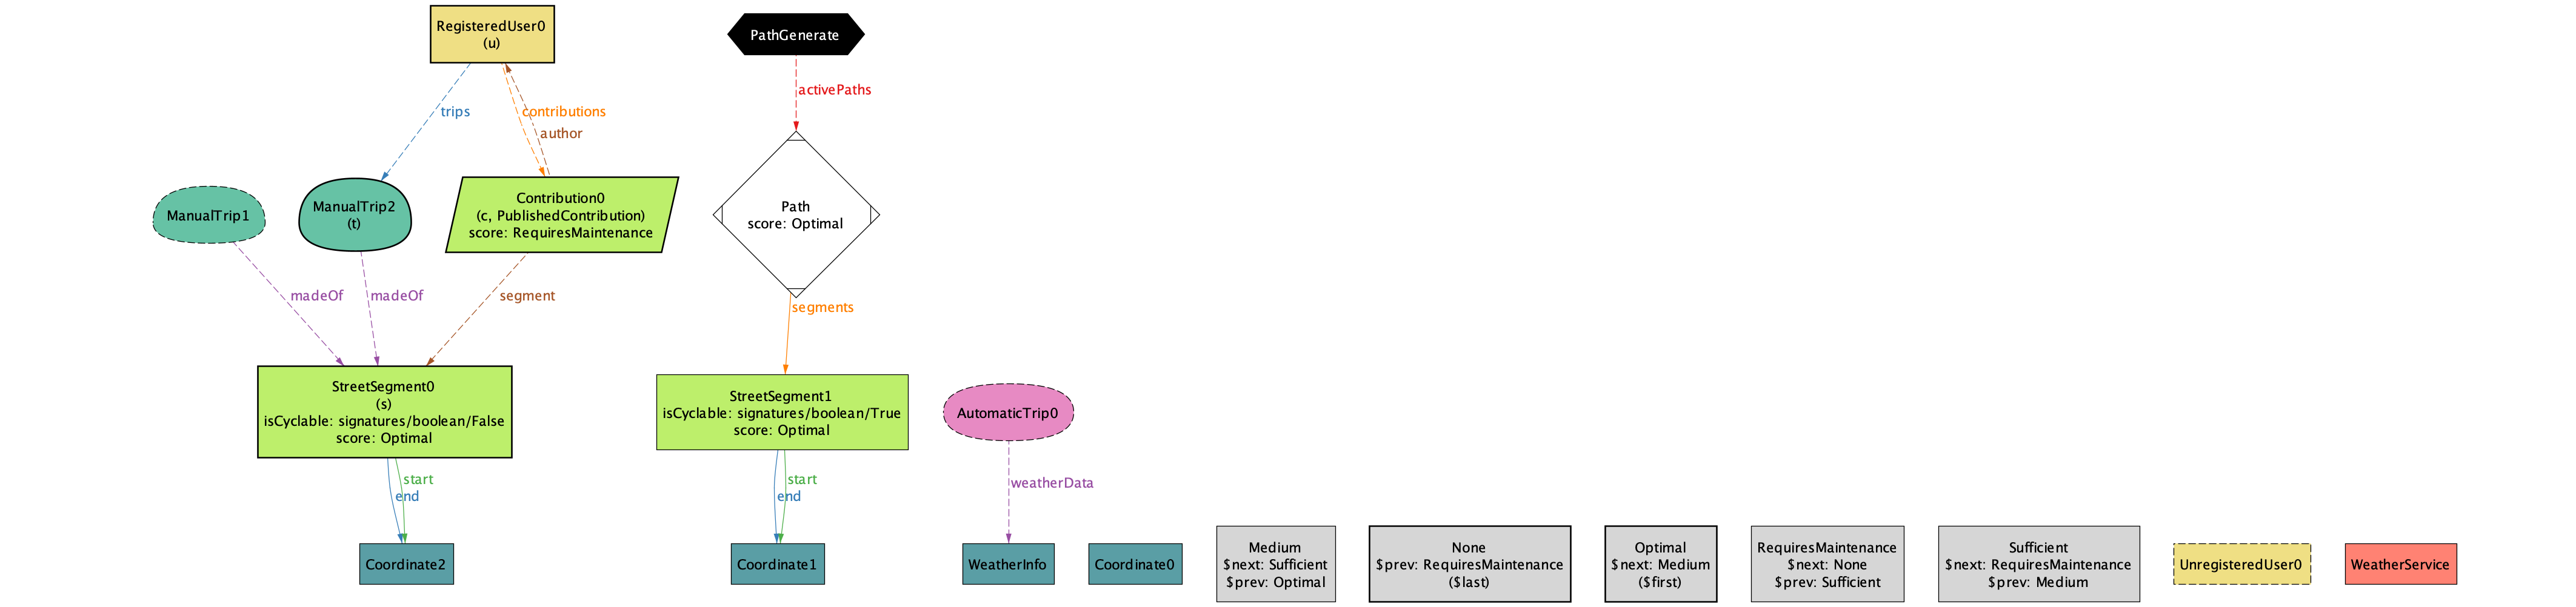
\includegraphics[width=\textwidth]{TestScenario_2.png}
    \caption{Dynamic World, Time 2: Contribution Publication}
    \label{fig:scenario_step2}
\end{figure}

Figure \ref{fig:scenario_step2} depicts the system state immediately after a Registered User saves a trip and publishes a contribution. The \texttt{Contribution0} object records a \texttt{RequiresMaintenance} score; however, the associated \texttt{StreetSegment0} still retains its initial \texttt{Optimal} status, correctly representing the pending state before data processing occurs.

\begin{figure}[H]
    \centering
    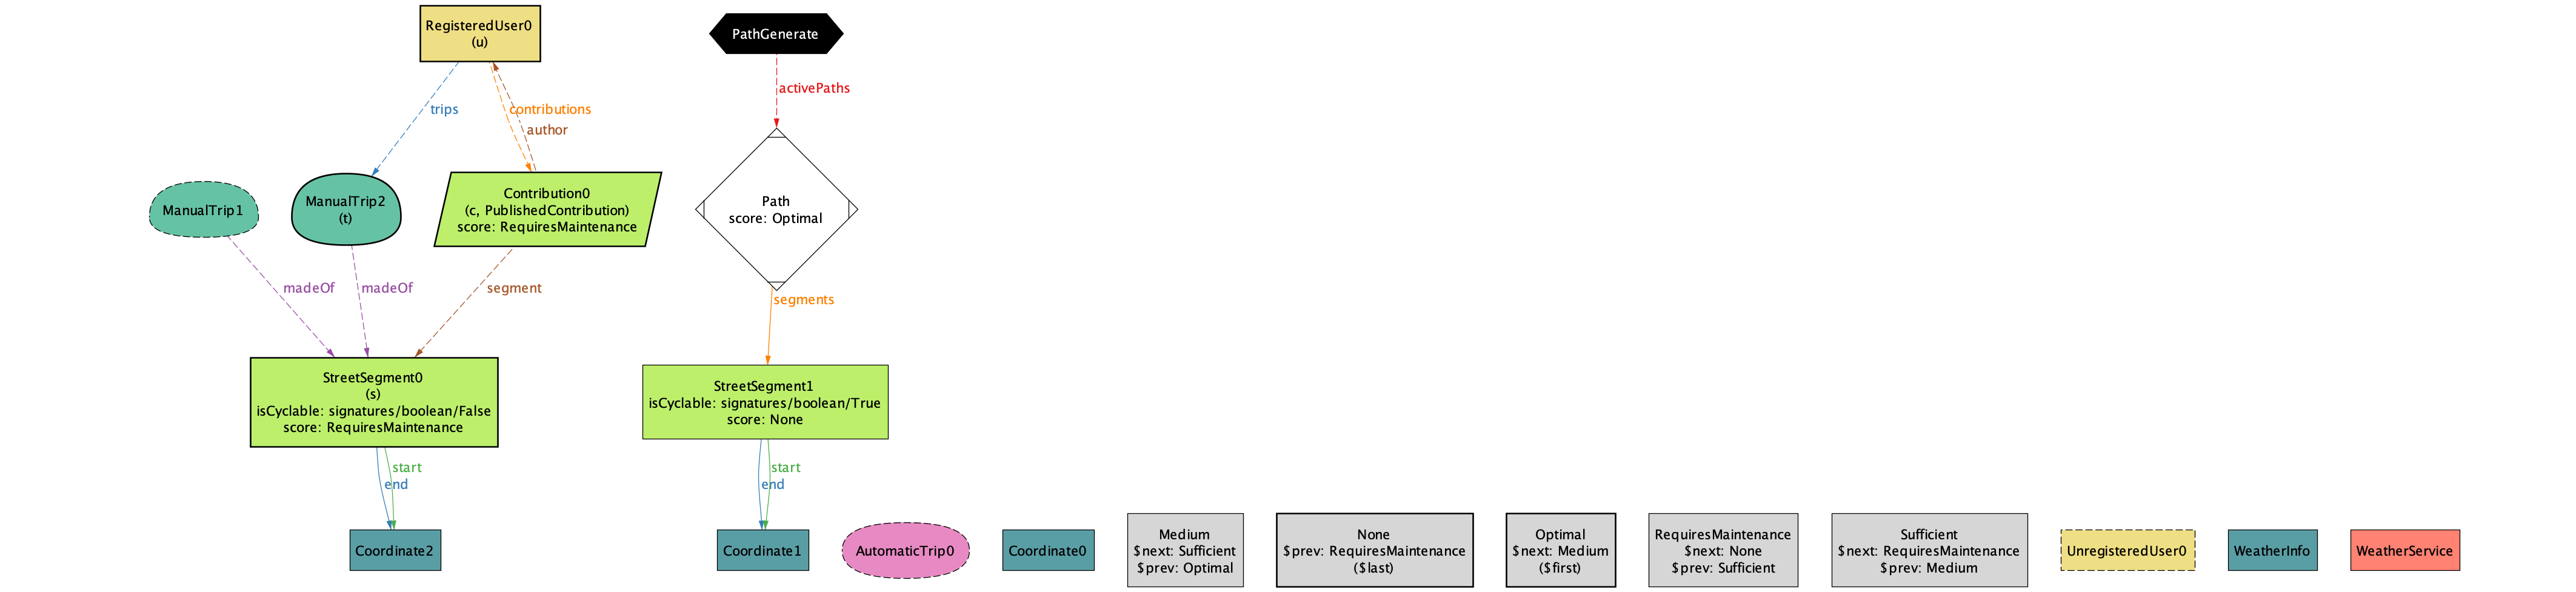
\includegraphics[width=\textwidth]{TestScenario_3.png}
    \caption{Dynamic World, Time 3: Data Merge and Update}
    \label{fig:scenario_step3}
\end{figure}

Figure \ref{fig:scenario_step3} shows the state after the execution of the \texttt{merge} predicate. The system aggregates the feedback, forcing an update on the map topology: \texttt{StreetSegment0} adopts the \texttt{RequiresMaintenance} score and its \texttt{isCyclable} attribute switches to \texttt{False}, confirming that the user's report successfully impacted the global knowledge.

\subsection{Scenario: Automatic Detection Confirmation}

This scenario validates the interaction where a user confirms a sensor detection during an automatic trip, transforming a raw system alert into a verified user contribution. The following instances correspond to the \texttt{TestDetectionConfirmation} predicate.

\begin{figure}[H]
    \centering
    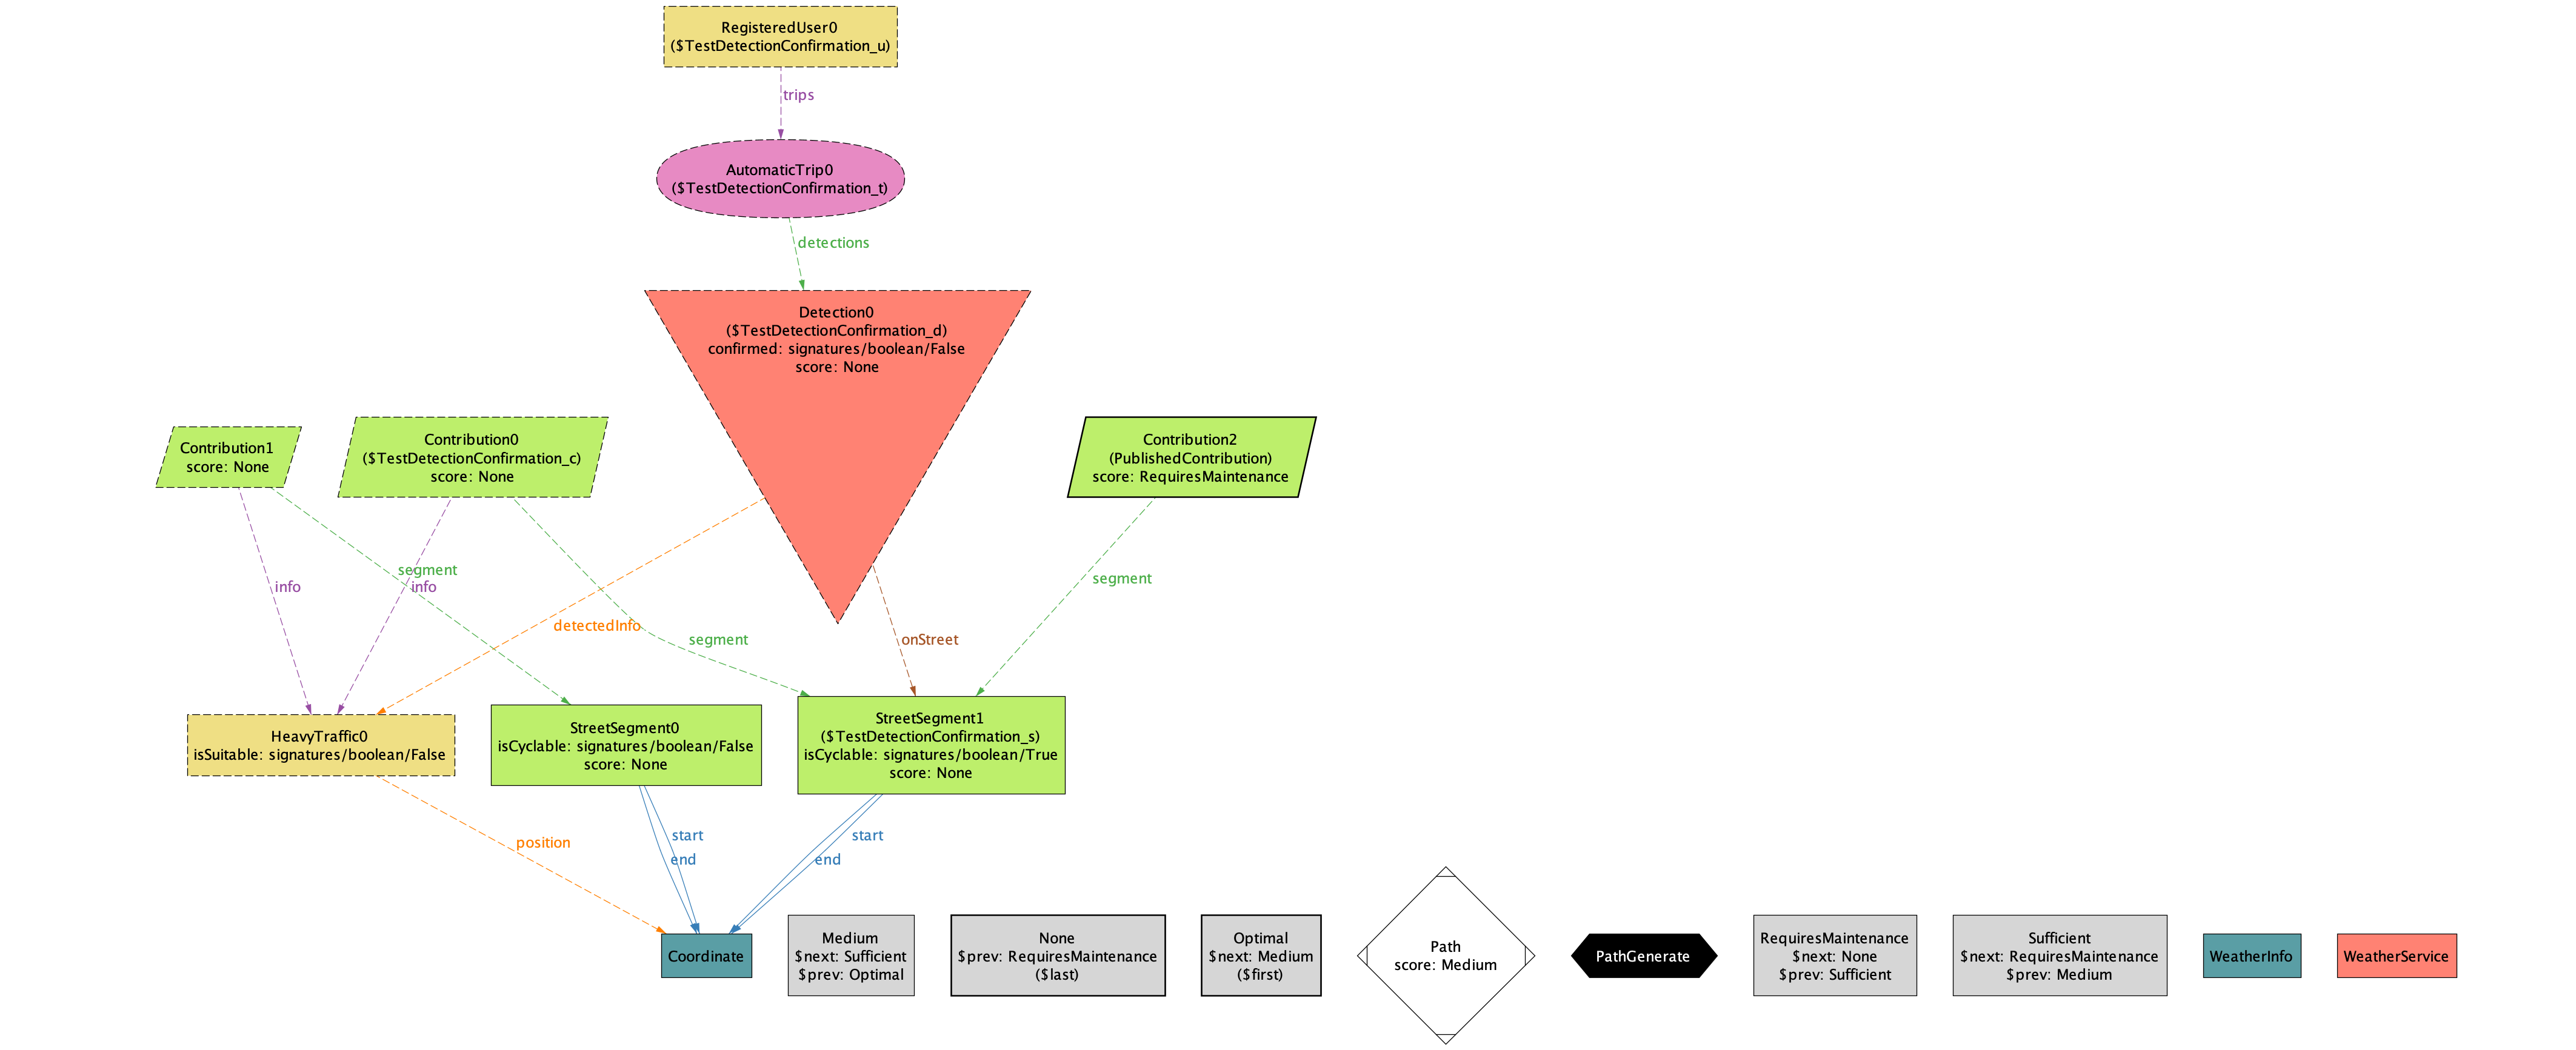
\includegraphics[width=\textwidth]{TestDetectionConfirmed_0.png}
    \caption{Dynamic World, Step 0: Unconfirmed Detection}
    \label{fig:detection_step0}
\end{figure}

Figure \ref{fig:detection_step0} illustrates the initial state of an \texttt{AutomaticTrip}. A \texttt{Detection} object (red triangle) is linked to the trip and a street segment, but its status is currently unconfirmed (\texttt{confirmed: False}). At this stage, the detection exists as raw data, and no formal \texttt{Contribution} is yet associated with the user or the trip.

\begin{figure}[H]
    \centering
    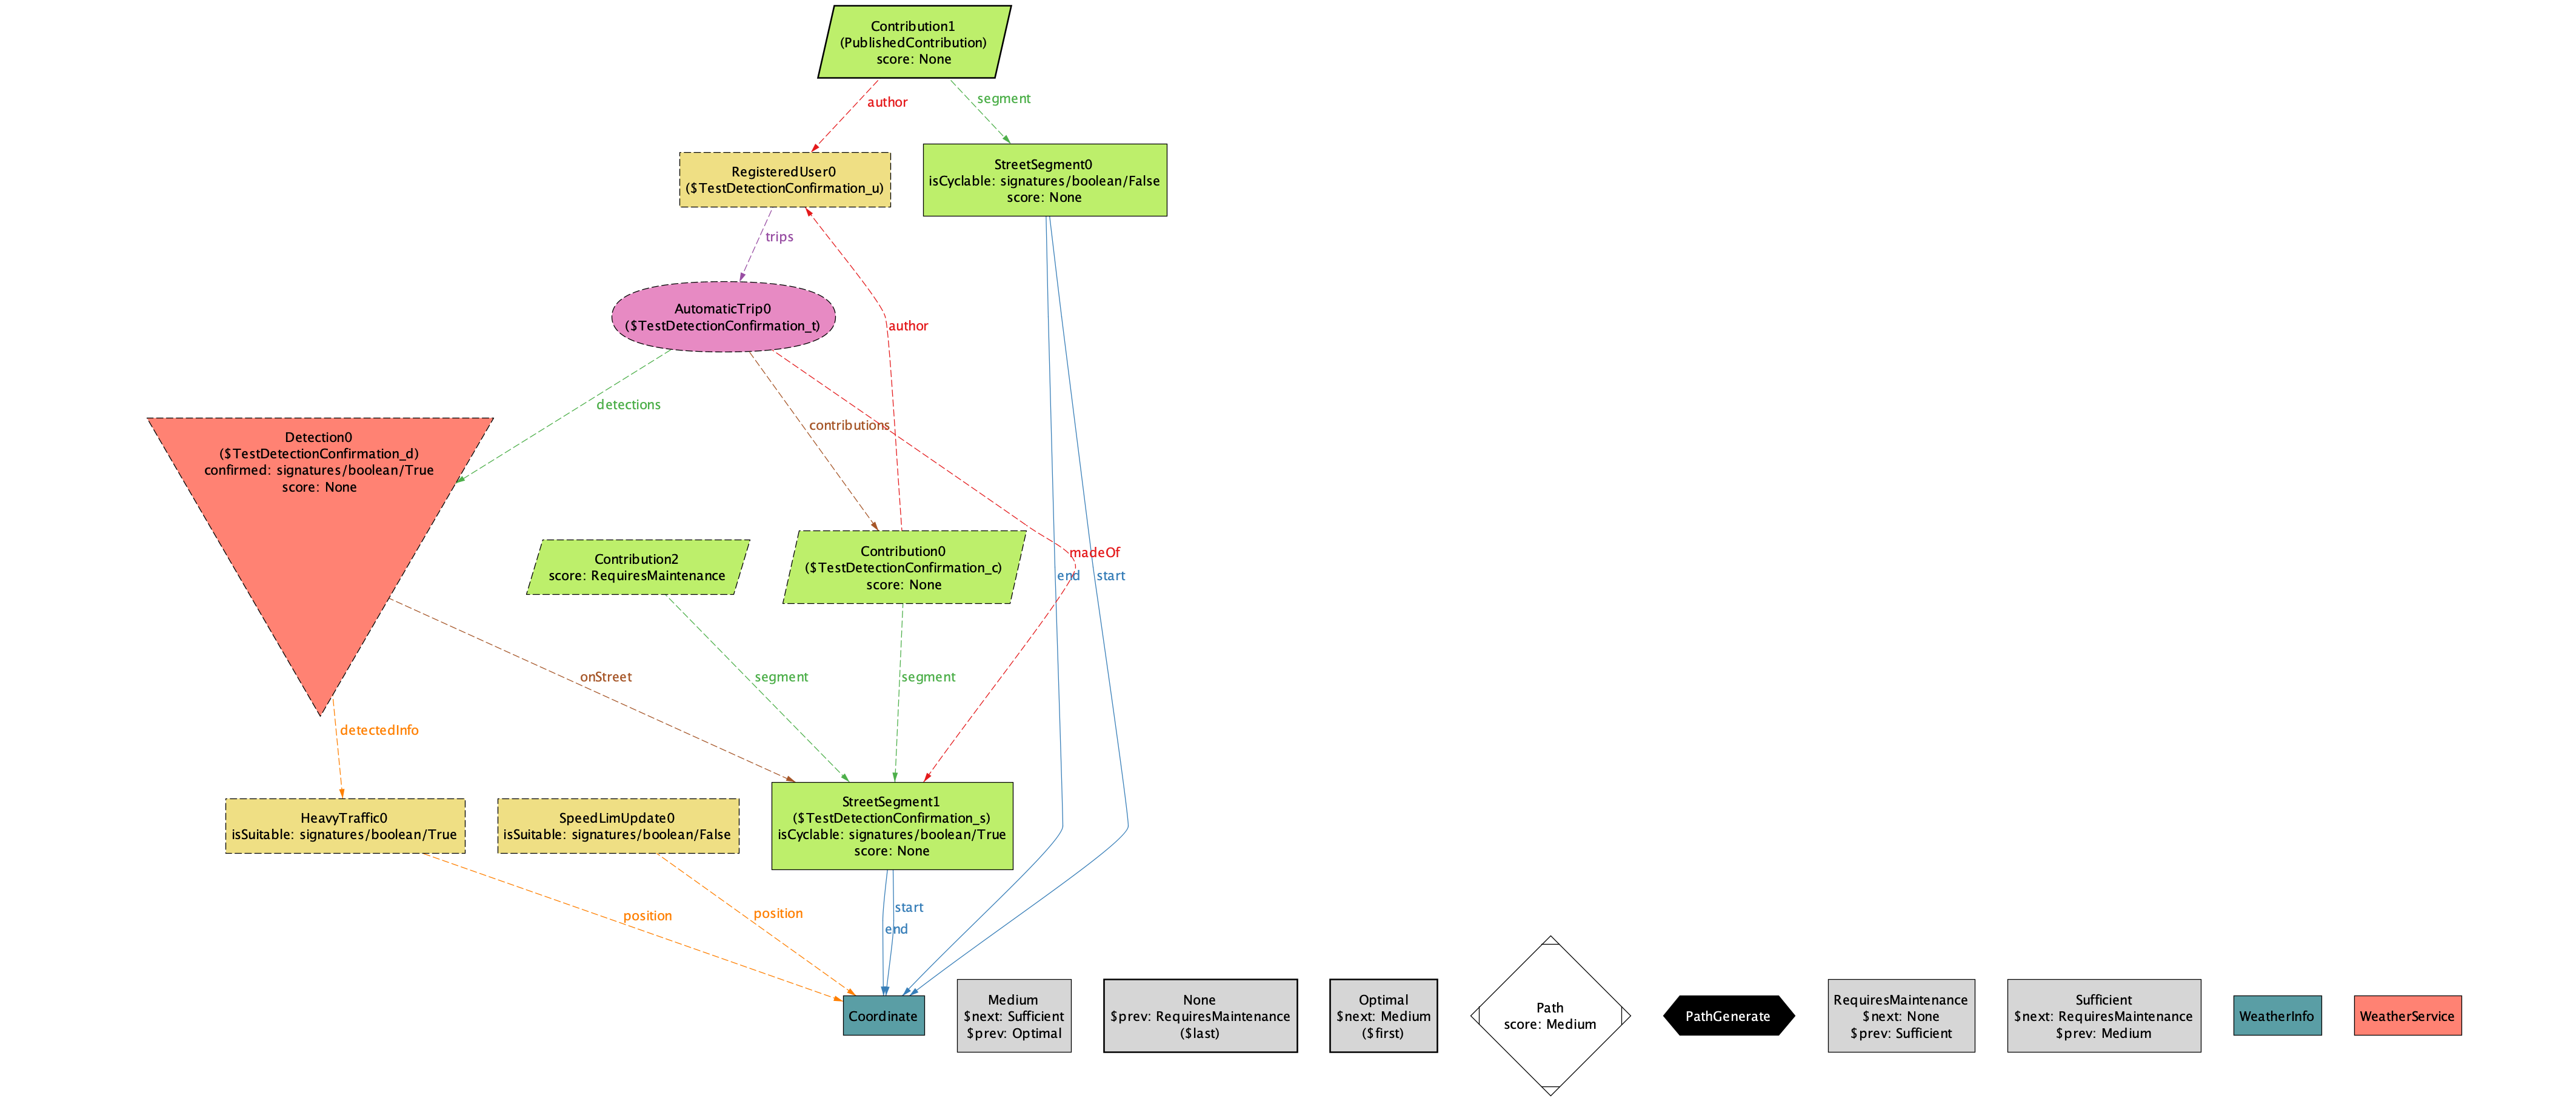
\includegraphics[width=\textwidth]{TestDetectionConfirmed_1.png}
    \caption{Dynamic World, Step 1: Confirmation and Contribution Generation}
    \label{fig:detection_step1}
\end{figure}

Figure \ref{fig:detection_step1} depicts the system state after the \texttt{confirmDetection} predicate is executed. The \texttt{Detection} status updates to \texttt{True}, and the system formally generates a new \texttt{Contribution}. This new object is now structurally linked to the \texttt{RegisteredUser} and the \texttt{AutomaticTrip}, inheriting the score and segment location from the original detection.


\subsection{Scenario: Path Invalidation and Independence}

This scenario demonstrates the system's topological consistency. It verifies that if a specific street segment becomes non-cyclable, only the paths utilizing that specific segment are invalidated, while intersecting or nearby paths remain active. The following instances correspond to the \texttt{PathBreakScenario} predicate.

\begin{figure}[H]
    \centering
    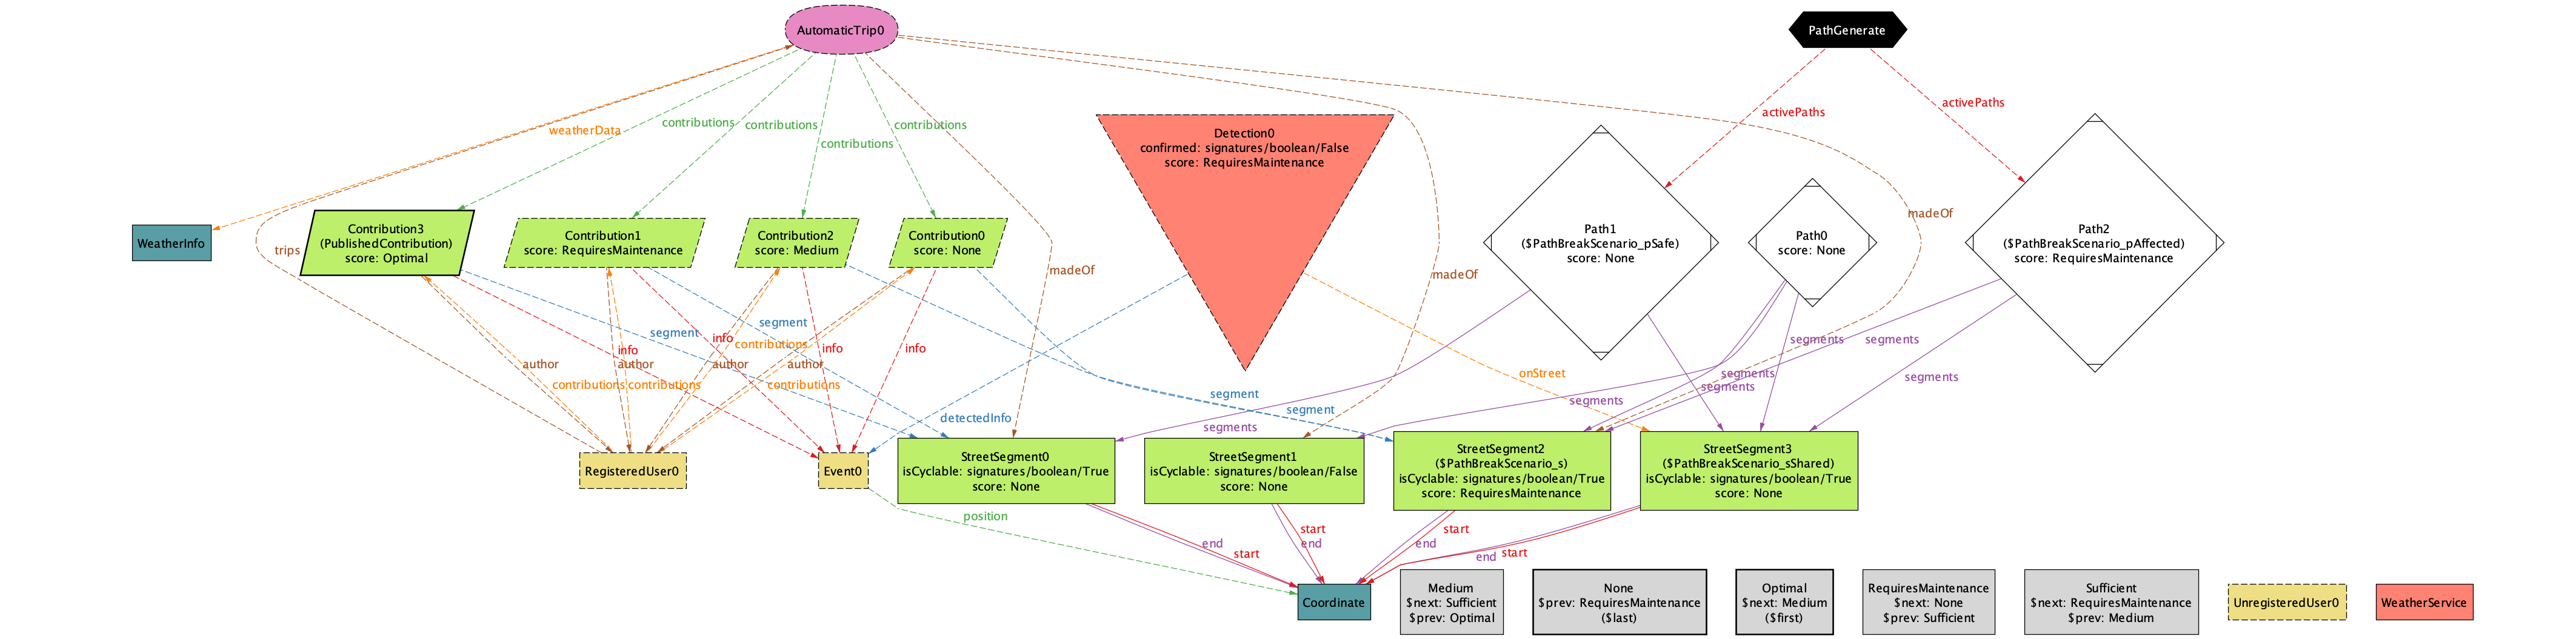
\includegraphics[width=\textwidth]{PathBreakScenario_0.png}
    \caption{Dynamic World, Step 0: Initial Connectivity}
    \label{fig:path_break_step0}
\end{figure}

Figure \ref{fig:path_break_step0} shows the initial system state with two distinct paths, \texttt{Path1} and \texttt{Path2} . Both paths are currently valid and included in \texttt{PathGenerate.activePaths} because all their constituent segments are cyclable. Notably, the paths share a common geometry (a shared segment), but \texttt{Path1} relies on a specific critical segment \texttt{s} that \texttt{Path2} does not use.

\begin{figure}[H]
    \centering
    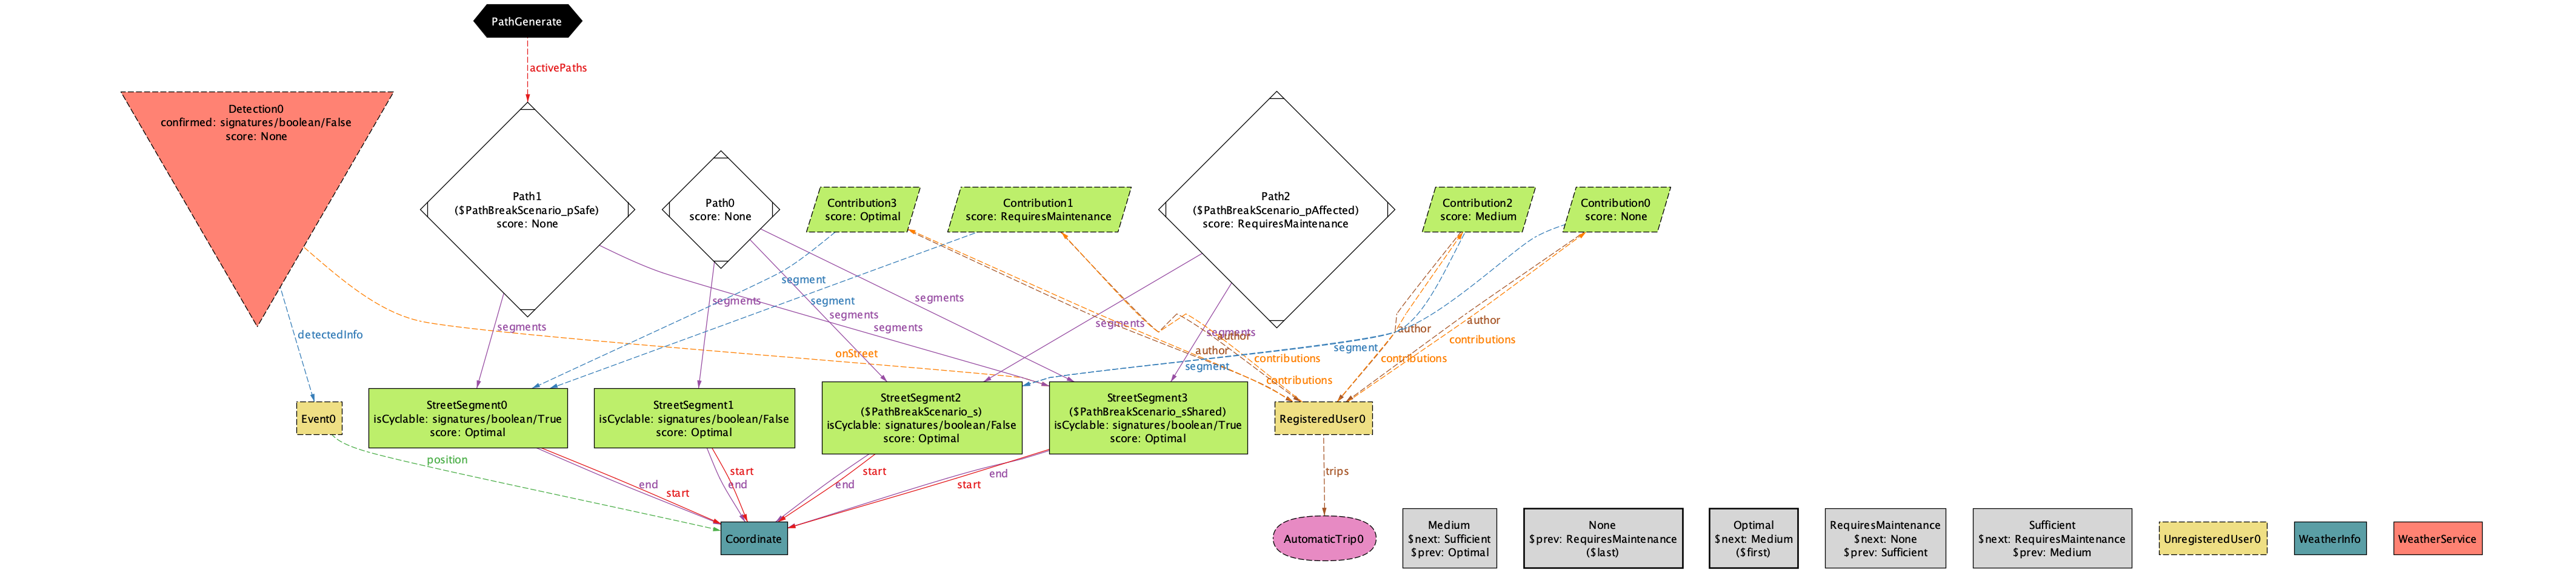
\includegraphics[width=\textwidth]{PathBreakScenario_1.png}
    \caption{Dynamic World, Step 1: Localized Failure}
    \label{fig:path_break_step1}
\end{figure}

Figure \ref{fig:path_break_step1} depicts the state after the critical segment \texttt{s} is marked as non-cyclable (\texttt{isCyclable: False}) . The system enforces the validity constraints: \texttt{Path1} is immediately removed from \texttt{activePaths}, while \texttt{Path2} remains active and unaffected. This proves that issues on a specific road segment are handled locally and do not cascade to invalidate unrelated or merely intersecting valid routes.



    \chapter{Effort Spent}
    \label{ch:effort_spent}%
    \begin{table}[H]
    \begin{center}
        \begin{tabular}{|c|c|}
            \hline
            Group Member & Effort Spent in each Section \\
            \hline
            David Ravelli & \begin{tabular}{p{0.25\linewidth}|c}
                             Introduction          & $4h$ \\
                             Overall Description   & $4h$ \\
                             Specific Requirements & $3h$ \\
                             Formal Analysis       & $14h$ \\
                             Reasoning             & $8h$ \\
            \end{tabular} \\
            \hline
            Francesco Rausa & \begin{tabular}{p{0.25\linewidth}|c}
                            Introduction          & $4h$ \\
                            Overall Description   & $6h$ \\
                            Specific Requirements & $13h$ \\
                            Formal Analysis       & $2h$  \\
                            Reasoning             & $8h$ \\
            \end{tabular} \\
            \hline
            Pietro Poggi & \begin{tabular}{p{0.25\linewidth}|c}
                            Introduction          & $4h$ \\
                            Overall Description   & $6h$ \\
                            Specific Requirements & $11h$ \\
                            Formal Analysis       & $4h$ \\
                            Reasoning             & $8h$ \\
            \end{tabular} \\
            \hline
        \end{tabular}
        \caption{Effort spent by each member of the group.}
        \label{tab:effort_spent}
    \end{center}
\end{table}


    \chapter{References}
    \label{ch:references}%
    \section{Used Tools}
\label{sec:used_tools}%

\begin{itemize}
    \item \textbf{Overleaf}: LaTeX collaborative writing.
    \item \textbf{Lucid Chart}: diagrams.
    \item \textbf{Alloy}: formal analysis for the system.
    \item \textbf{ChatGPT}: Used as a writing support tool for text refinement and linguistic revision. 
No requirements or design decisions were automatically generated without human validation.

\end{itemize}

% LIST OF FIGURES
    \listoffigures

    \cleardoublepage


\end{document}
